%% This documentation was generated with Faust version 2.28.0
%% Tue Jan 26 20:15:17 2021
%% https://faust.grame.fr

\documentclass{article}

\usepackage[utf8]{inputenc}
\usepackage{graphicx}
\usepackage[usenames]{color}
\usepackage{listings}
\usepackage{supertabular}
\usepackage{amsmath}
\usepackage{latexsym, amssymb}
\usepackage{breqn}

% No indent
\setlength{\parindent}{0pt}

% Make LaTeX output a dot when typing an asterisk
\DeclareMathSymbol{*}{\mathbin}{symbols}{"01}

% lstlistings setup
\definecolor{yobg}{rgb}{0.9,0.9,1}
\definecolor{yotxt}{rgb}{0.01,0.01,0.52} % a dark blue.
\definecolor{mylstbg}{rgb}{0.98,0.98,0.98} % a really pale grey.
\definecolor{mylstcmt}{rgb}{0.01,0.52,0.01} % a dark green.
\definecolor{mylstdoc}{rgb}{0.80,0.30,0.80} % a medium pink.

\lstset{%
  language=C++, 
  numbers=left,%none,
  tabsize=4, 
  frame=single, 
  breaklines=true, 
  numberstyle=\tiny\ttfamily, 
  backgroundcolor=\color{mylstbg}, 
  basicstyle=\scriptsize\ttfamily, 
  commentstyle=\slshape\color{mylstcmt}, %\itshape,
  frameround=tttt, 
  columns=flexible, %fixed, 
  showstringspaces=false,
  emptylines=2,
  inputencoding=utf8,
  extendedchars=true,
  literate=	{á}{{\'a}}1 
			{à}{{\`a}}1 
			{ä}{{\"a}}1 
			{â}{{\^a}}1
			{é}{{\'e}}1 
			{è}{{\`e}}1 
			{ë}{{\"e}}1 
			{ê}{{\^e}}1
			{ï}{{\"i}}1 
			{î}{{\^i}}1
			{ö}{{\"o}}1 
			{ô}{{\^o}}1
			{è}{{\`e}}1 
			{ù}{{\`u}}1 
			{û}{{\^u}}1
			{ç}{{\c{c}}}1 
			{Ç}{{\c{C}}}1,
  emph={component, declare, environment, import, library, process},
  emph={[2]ffunction, fconstant, fvariable},
  emph={[3]button, checkbox, vslider, hslider, nentry, vgroup, hgroup, tgroup, vbargraph, hbargraph, attach},
  emphstyle=\color{yotxt}, %\underline, %\bfseries,
  morecomment=[s][\color{mylstdoc}]{<mdoc>}{</mdoc>},
  rulecolor=\color{black}
}

\newcommand{\faustfilename}{src/generic_snarefs.dsp}
\newcommand{\faustdocdir}{generic_snarefs-mdoc}
\newcommand{\faustprogname}{generic_snarefs}
\newcommand{\faustversion}{2.28.0}
\newcommand{\faustdocdate}{January 26, 2021}

\begin{document}
\title{generic_snarefs} \author{ Henrik Frisk ,  henrikfr } \date{\today} \maketitle \begin{tabular}{ll}  \hline  \textbf{author} &  Henrik Frisk ,  henrikfr  \\  \textbf{basics.lib/name} & Faust Basic Element Library \\  \textbf{basics.lib/version} & 0.1 \\  \textbf{copyright} & (c) dinergy 2018  \\  \textbf{envelopes.lib/ar:author} & Yann Orlarey, Stéphane Letz \\  \textbf{envelopes.lib/author} & GRAME \\  \textbf{envelopes.lib/copyright} & GRAME \\  \textbf{envelopes.lib/license} & LGPL with exception \\  \textbf{envelopes.lib/name} & Faust Envelope Library \\  \textbf{envelopes.lib/version} & 0.1 \\  \textbf{filename} & generic_snarefs.dsp \\  \textbf{filters.lib/lowpass0_highpass1} & MIT-style STK-4.3 license, Copyright (C) 2003-2019 by Julius O. Smith III <jos@ccrma.stanford.edu> \\  \textbf{filters.lib/name} & Faust Filters Library \\  \textbf{filters.lib/pole:author} & Julius O. Smith III \\  \textbf{filters.lib/pole:copyright} & Copyright (C) 2003-2019 by Julius O. Smith III <jos@ccrma.stanford.edu> \\  \textbf{filters.lib/pole:license} & MIT-style STK-4.3 license \\  \textbf{license} &  BSD  \\  \textbf{math.lib/author} & GRAME \\  \textbf{math.lib/copyright} & GRAME \\  \textbf{math.lib/deprecated} & This library is deprecated and is not maintained anymore. It will be removed in August 2017. \\  \textbf{math.lib/license} & LGPL with exception \\  \textbf{math.lib/name} & Math Library \\  \textbf{math.lib/version} & 1.0 \\  \textbf{maths.lib/author} & GRAME \\  \textbf{maths.lib/copyright} & GRAME \\  \textbf{maths.lib/license} & LGPL with exception \\  \textbf{maths.lib/name} & Faust Math Library \\  \textbf{maths.lib/version} & 2.3 \\  \textbf{music.lib/author} & GRAME \\  \textbf{music.lib/copyright} & GRAME \\  \textbf{music.lib/deprecated} & This library is deprecated and is not maintained anymore. It will be removed in August 2017. \\  \textbf{music.lib/license} & LGPL with exception \\  \textbf{music.lib/name} & Music Library \\  \textbf{music.lib/version} & 1.0 \\  \textbf{name} & generic_snarefs \\  \textbf{noises.lib/name} & Faust Noise Generator Library \\  \textbf{noises.lib/version} & 0.0 \\  \textbf{oscillators.lib/name} & Faust Oscillator Library \\  \textbf{oscillators.lib/version} & 0.1 \\  \textbf{platform.lib/name} & Generic Platform Library \\  \textbf{platform.lib/version} & 0.1 \\  \textbf{signals.lib/name} & Faust Signal Routing Library \\  \textbf{signals.lib/version} & 0.0 \\  \textbf{version} &  0.1  \\  \hline \end{tabular} \bigskip  \bigskip This document provides a mathematical description of the Faust program text stored in the \texttt{\faustfilename} file. See the notice in Section\,\ref{notice} (page\,\pageref{notice}) for details.   \section{Mathematical definition of \texttt{process}} \label{equation}  The \emph{\faustprogname} program evaluates the signal transformer denoted by \texttt{process}, which is mathematically defined as follows: 
% Set of Faust formulas (corresponding to an <equation> tag).
\begin{enumerate}

\item Output signals $y_i$ for $i \in [1,2]$ such that
	\begin{dgroup*}
		\begin{dmath*}
				y_{1}(t) = x(t)
		\end{dmath*}
		\begin{dmath*}
				y_{2}(t) = {u_s}_{10}(t) * \max\left( 0, \min\left( \frac{r_{19}(t)}{s_{16}(t)}, \frac{s_{16}(t) - r_{19}(t)}{\max\left( 1, k_{1} * r_{31}(t) \right)} + 1 \right) \right) *  \left(0.1 * v_{1}[\mathrm{int}\left(65536 * r_{29}(t)\right)] + s_{6}(t) + s_{5}(t) + s_{15}(t) + s_{15}(t) + 0.1 * v_{1}[\mathrm{int}\left(65536 * r_{17}(t)\right)] + s_{6}(t) - s_{5}(t)\right) 
		\end{dmath*}
	\end{dgroup*}

\item Input signal $x$ 

\item User-interface input signals  ${u_s}_i$ for $i \in [1,10]$ such that
\begin{itemize}
	\item \textsf{snare/}
		\begin{center}
			\begin{supertabular}{lll}
				\textsf{"filter sweep"}  & ${u_s}_{1}(t)$ $\in$ $\left[\,0, 2\,\right]$ & $(\mbox{default value} = 1)$\\
				\textsf{"triangle freq"}  & ${u_s}_{2}(t)$ $\in$ $\left[\,50, 2000\,\right]$ & $(\mbox{default value} = 111)$\\
				\textsf{"osc 2 freq"}  & ${u_s}_{3}(t)$ $\in$ $\left[\,50, 2000\,\right]$ & $(\mbox{default value} = 180)$\\
				\textsf{"noise attack"}  & ${u_s}_{4}(t)$ $\in$ $\left[\,0, 0.1\,\right]$ & $(\mbox{default value} = 1 * 10^{-08})$\\
				\textsf{"noise rel"}  & ${u_s}_{5}(t)$ $\in$ $\left[\,1 * 10^{-07}, 0.5\,\right]$ & $(\mbox{default value} = 0.1)$\\
				\textsf{"noise lvl"}  & ${u_s}_{6}(t)$ $\in$ $\left[\,0, 1.5\,\right]$ & $(\mbox{default value} = 0.1)$\\
				\textsf{"osc 1 freq"}  & ${u_s}_{7}(t)$ $\in$ $\left[\,50, 2000\,\right]$ & $(\mbox{default value} = 330)$\\
				\textsf{"attack"}  & ${u_s}_{8}(t)$ $\in$ $\left[\,0, 0.1\,\right]$ & $(\mbox{default value} = 1 * 10^{-08})$\\
				\textsf{"rel"}  & ${u_s}_{9}(t)$ $\in$ $\left[\,1 * 10^{-07}, 0.5\,\right]$ & $(\mbox{default value} = 0.1)$\\
				\textsf{"amp"}  & ${u_s}_{10}(t)$ $\in$ $\left[\,0, 2\,\right]$ & $(\mbox{default value} = 0.5)$\\
			\end{supertabular}
		\end{center}
	\end{itemize}

\item Intermediate signals  $p_i$ for $i \in [1,20]$,  $s_i$ for $i \in [1,16]$,  $r_i$ for $i \in [1,28]$ and  $v_1$ such that
	\begin{dgroup*}
		\begin{dmath*}
				p_{1}(t) = \max\left( {u_s}_{2}(t), 23.4489496824621 \right)
		\end{dmath*}
		\begin{dmath*}
				p_{2}(t) = \max\left( 20, \left\lvert{p_{1}(t)}\right\rvert \right)
		\end{dmath*}
		\begin{dmath*}
				p_{3}(t) = k_{2} * p_{2}(t)
		\end{dmath*}
		\begin{dmath*}
				p_{4}(t) = \frac{k_{3}}{p_{2}(t)}
		\end{dmath*}
		\begin{dmath*}
				p_{5}(t) = \max\left( 0, \min\left( 2047, \frac{k_{4}}{p_{1}(t)} \right) \right)
		\end{dmath*}
		\begin{dmath*}
				p_{6}(t) = \mathrm{int}\left(p_{5}(t)\right)
		\end{dmath*}
		\begin{dmath*}
				p_{7}(t) = \mathrm{int}\left(p_{6}(t) \oplus 1\right)
		\end{dmath*}
		\begin{dmath*}
				p_{8}(t) = \left\lfloor {p_{5}(t)} \right\rfloor
		\end{dmath*}
		\begin{dmath*}
				p_{9}(t) =  \left(p_{5}(t) - p_{8}(t)\right) 
		\end{dmath*}
		\begin{dmath*}
				p_{10}(t) =  \left(p_{8}(t) + 1 - p_{5}(t)\right) 
		\end{dmath*}
		\begin{dmath*}
				p_{11}(t) = \frac{k_{6}}{{u_s}_{2}(t)}
		\end{dmath*}
		\begin{dmath*}
				p_{12}(t) = k_{7} * {u_s}_{2}(t)
		\end{dmath*}
		\begin{dmath*}
				p_{13}(t) = k_{8} * {u_s}_{2}(t)
		\end{dmath*}
		\begin{dmath*}
				p_{14}(t) = k_{9} * {u_s}_{2}(t)
		\end{dmath*}
		\begin{dmath*}
				p_{15}(t) = k_{2} * {u_s}_{3}(t)
		\end{dmath*}
		\begin{dmath*}
				p_{16}(t) = 0.9 * {u_s}_{4}(t)
		\end{dmath*}
		\begin{dmath*}
				p_{17}(t) = 0.8 * {u_s}_{5}(t)
		\end{dmath*}
		\begin{dmath*}
				p_{18}(t) = k_{2} * {u_s}_{7}(t)
		\end{dmath*}
		\begin{dmath*}
				p_{19}(t) = 0.9 * {u_s}_{8}(t)
		\end{dmath*}
		\begin{dmath*}
				p_{20}(t) = 0.8 * {u_s}_{9}(t)
		\end{dmath*}
	\end{dgroup*}


	\begin{dgroup*}
		\begin{dmath*}
				s_{1}(t) = {2 * r_{4}(t) + -1}^{2}
		\end{dmath*}
		\begin{dmath*}
				s_{2}(t) = p_{4}(t) * r_{2}(t\!-\!1) *  \left(s_{1}(t) - s_{1}(t\!-\!1)\right) 
		\end{dmath*}
		\begin{dmath*}
				s_{3}(t) = p_{12}(t) * r_{3}(t) * r_{1}(t)\pmod{\frac{p_{11}(t)}{r_{3}(t)}}
		\end{dmath*}
		\begin{dmath*}
				s_{4}(t) = p_{13}(t) * r_{3}(t)
		\end{dmath*}
		\begin{dmath*}
				s_{5}(t) = r_{7}(t) * \cos\left(s_{3}(t)\right)
		\end{dmath*}
		\begin{dmath*}
				s_{6}(t) = r_{12}(t) * \sin\left(s_{3}(t)\right)
		\end{dmath*}
		\begin{dmath*}
				s_{7}(t) = \max\left( 1, k_{1} * r_{18}(t) \right)
		\end{dmath*}
		\begin{dmath*}
				s_{8}(t) = 1103515245 \odot  \left(r_{22}(t\!-\!1) \oplus 12345\right) 
		\end{dmath*}
		\begin{dmath*}
				s_{9}(t) = 1103515245 \odot  \left(s_{8}(t) \oplus 12345\right) 
		\end{dmath*}
		\begin{dmath*}
				s_{10}(t) = 1103515245 \odot  \left(s_{9}(t) \oplus 12345\right) 
		\end{dmath*}
		\begin{dmath*}
				s_{11}(t) = 1103515245 \odot  \left(s_{10}(t) \oplus 12345\right) 
		\end{dmath*}
		\begin{dmath*}
				s_{12}(t) = 1103515245 \odot  \left(s_{11}(t) \oplus 12345\right) 
		\end{dmath*}
		\begin{dmath*}
				s_{13}(t) = 1103515245 \odot  \left(s_{12}(t) \oplus 12345\right) 
		\end{dmath*}
		\begin{dmath*}
				s_{14}(t) = 1103515245 \odot  \left(s_{13}(t) \oplus 12345\right) 
		\end{dmath*}
		\begin{dmath*}
				s_{15}(t) = {u_s}_{6}(t) *  \left(4.6566128752458 * 10^{-10} * r_{22}(t) + 4.6566128752458 * 10^{-10} * r_{28}(t) + 4.6566128752458 * 10^{-10} * r_{27}(t) + 4.6566128752458 * 10^{-10} * r_{26}(t) + 4.6566128752458 * 10^{-10} * r_{25}(t) + 4.6566128752458 * 10^{-10} * r_{24}(t) + 4.6566128752458 * 10^{-10} * r_{23}(t) + 4.6566128752458 * 10^{-10} * r_{21}(t)\right)  * \max\left( 0, \min\left( \frac{r_{19}(t)}{s_{7}(t)}, \frac{s_{7}(t) - r_{19}(t)}{\max\left( 1, k_{1} * r_{20}(t) \right)} + 1 \right) \right)
		\end{dmath*}
		\begin{dmath*}
				s_{16}(t) = \max\left( 1, k_{1} * r_{30}(t) \right)
		\end{dmath*}
	\end{dgroup*}


	\begin{dgroup*}
		\begin{dmath*}
				r_{2}(t) = 1
		\end{dmath*}
		\begin{dmath*}
				r_{1}(t) = {u_s}_{1}(t) + r_{1}(t\!-\!1)
		\end{dmath*}
		\begin{dmath*}
				r_{4}(t) = p_{3}(t) + r_{4}(t\!-\!1) - \left\lfloor {p_{3}(t) + r_{4}(t\!-\!1)} \right\rfloor
		\end{dmath*}
		\begin{dmath*}
				r_{3}(t) =  \left(0.999 * r_{3}(t\!-\!1) + s_{2}(t)\right)  -  \left(p_{10}(t) * s_{2}(t\!-\!p_{6}(t)) + p_{9}(t) * s_{2}(t\!-\!p_{7}(t))\right) 
		\end{dmath*}
		\begin{dmath*}
				r_{10}(t) = 0.479401 *  \left(s_{4}(t\!-\!1) + r_{10}(t\!-\!2)\right)  - s_{4}(t\!-\!3)
		\end{dmath*}
		\begin{dmath*}
				r_{9}(t) = 0.876218 *  \left(r_{10}(t) + r_{9}(t\!-\!2)\right)  - r_{10}(t\!-\!2)
		\end{dmath*}
		\begin{dmath*}
				r_{8}(t) = 0.976599 *  \left(r_{9}(t) + r_{8}(t\!-\!2)\right)  - r_{9}(t\!-\!2)
		\end{dmath*}
		\begin{dmath*}
				r_{7}(t) = 0.9975 *  \left(r_{8}(t) + r_{7}(t\!-\!2)\right)  - r_{8}(t\!-\!2)
		\end{dmath*}
		\begin{dmath*}
				r_{15}(t) =  \left(0.161758 * r_{15}(t\!-\!2) + p_{14}(t) * r_{3}(t)\right)  - s_{4}(t\!-\!2)
		\end{dmath*}
		\begin{dmath*}
				r_{14}(t) = 0.733029 *  \left(r_{15}(t) + r_{14}(t\!-\!2)\right)  - r_{15}(t\!-\!2)
		\end{dmath*}
		\begin{dmath*}
				r_{13}(t) = 0.94535 *  \left(r_{14}(t) + r_{13}(t\!-\!2)\right)  - r_{14}(t\!-\!2)
		\end{dmath*}
		\begin{dmath*}
				r_{12}(t) = 0.990598 *  \left(r_{13}(t) + r_{12}(t\!-\!2)\right)  - r_{13}(t\!-\!2)
		\end{dmath*}
		\begin{dmath*}
				r_{16}(t) = r_{16}(t\!-\!1) \oplus 1
		\end{dmath*}
		\begin{dmath*}
				r_{17}(t) = p_{15}(t) + r_{17}(t\!-\!1) - \left\lfloor {p_{15}(t) + r_{17}(t\!-\!1)} \right\rfloor
		\end{dmath*}
		\begin{dmath*}
				r_{18}(t) = p_{16}(t) + 0.1 * r_{18}(t\!-\!1)
		\end{dmath*}
		\begin{dmath*}
				r_{19}(t) =  \left(r_{19}(t\!-\!1) \oplus  \left(r_{19}(t\!-\!1) \hiderel{>} 0\right) \right)  \odot  \left(x(t) \hiderel{\leq} x(t\!-\!1)\right)  \oplus  \left(x(t) \hiderel{>} x(t\!-\!1)\right) 
		\end{dmath*}
		\begin{dmath*}
				r_{20}(t) = p_{17}(t) + 0.2 * r_{20}(t\!-\!1)
		\end{dmath*}
		\begin{dmath*}
				r_{22}(t) = 1103515245 \odot  \left(s_{14}(t) \oplus 12345\right) 
		\end{dmath*}
		\begin{dmath*}
				r_{21}(t) = s_{8}(t)
		\end{dmath*}
		\begin{dmath*}
				r_{23}(t) = s_{9}(t)
		\end{dmath*}
		\begin{dmath*}
				r_{24}(t) = s_{10}(t)
		\end{dmath*}
		\begin{dmath*}
				r_{25}(t) = s_{11}(t)
		\end{dmath*}
		\begin{dmath*}
				r_{26}(t) = s_{12}(t)
		\end{dmath*}
		\begin{dmath*}
				r_{27}(t) = s_{13}(t)
		\end{dmath*}
		\begin{dmath*}
				r_{28}(t) = s_{14}(t)
		\end{dmath*}
		\begin{dmath*}
				r_{29}(t) = p_{18}(t) + r_{29}(t\!-\!1) - \left\lfloor {p_{18}(t) + r_{29}(t\!-\!1)} \right\rfloor
		\end{dmath*}
		\begin{dmath*}
				r_{30}(t) = p_{19}(t) + 0.1 * r_{30}(t\!-\!1)
		\end{dmath*}
		\begin{dmath*}
				r_{31}(t) = p_{20}(t) + 0.2 * r_{31}(t\!-\!1)
		\end{dmath*}
	\end{dgroup*}


	\begin{dgroup*}
		\begin{dmath*}
				v_{1}[t] = \sin\left(9.58737992428526 * 10^{-05} *  \left(r_{16}(t) \oplus -1\right) \right) \condition{when $t \in [0,65535]$} 
		\end{dmath*}
	\end{dgroup*}

\item Constants $k_i$ for $i \in [1,9]$ such that
	\begin{dgroup*}
		\begin{dmath*}
				k_{1} = \min\left( 192000, \max\left( 1, f_S \right) \right)
		\end{dmath*}
		\begin{dmath*}
				k_{2} = \frac{1}{k_{1}}
		\end{dmath*}
		\begin{dmath*}
				k_{3} = 0.25 * k_{1}
		\end{dmath*}
		\begin{dmath*}
				k_{4} = 0.5 * k_{1}
		\end{dmath*}
		\begin{dmath*}
				k_{5} = f_S * k_{1}
		\end{dmath*}
		\begin{dmath*}
				k_{6} = 2.5 * k_{5}
		\end{dmath*}
		\begin{dmath*}
				k_{7} = \frac{2.51327412}{k_{5}}
		\end{dmath*}
		\begin{dmath*}
				k_{8} = \frac{0.4}{k_{1}}
		\end{dmath*}
		\begin{dmath*}
				k_{9} = \frac{0.0647032}{k_{1}}
		\end{dmath*}
	\end{dgroup*}

\end{enumerate}

 \section{Block diagram of \texttt{process}} \label{diagram}  The block diagram of \texttt{process} is shown on Figure\,\ref{figure1} (page\,\pageref{figure1}). \begin{figure}[ht!]
	\centering
	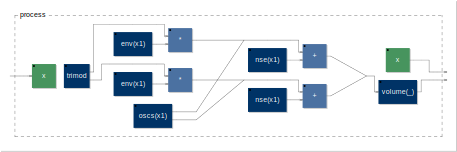
\includegraphics[width=\textwidth]{../svg/svg-01/process}
	\caption{Block diagram of \texttt{process}}
	\label{figure1}
\end{figure}

 \section{Notice} \label{notice}  
\begin{itemize}
	\item This document was generated using Faust version \faustversion\ on \faustdocdate.
	\item The value of a Faust program is the result of applying the signal transformer denoted by the expression to which the \texttt{process} identifier is bound to input signals, running at the $f_S$ sampling frequency.
	\item Faust (\emph{Functional Audio Stream}) is a functional programming language designed for synchronous real-time signal processing and synthesis applications. A Faust program is a set of bindings of identifiers to expressions that denote signal transformers. A signal $s$ in $S$ is a function mapping\footnote{Faust assumes that $\forall \, s \in S, \forall \, t \in \mathbb{Z}, s(t) = 0 \mathrm{\ when\ } t < 0$.} times $t \in \mathbb{Z}$ to values $s(t) \in \mathbb{R}$, while a signal transformer is a function from $S^n$ to $S^m$, where $n,m\in \mathbb{N}$. See the Faust manual for additional information (\textsf{http://faust.grame.fr}).
	\item Every mathematical formula derived from a Faust expression is assumed, in this document, to having been normalized (in an implementation-depen\-dent manner) by the Faust compiler.
	\item A block diagram is a graphical representation of the Faust binding of an identifier I to an expression E; each graph is put in a box labeled by I. Subexpressions of E are recursively displayed as long as the whole picture fits in one page.
	\item $\forall \, x \in \mathbb{R}$, 
	\begin{displaymath}
		\mathrm{int}(x) =
		\left\{\begin{array}{cl}
			\lfloor x \rfloor & \mbox{if \,} x > 0 \\
			\lceil x \rceil & \mbox{if \,} x < 0 \\
			0 & \mbox{if \,} x = 0 \\
		\end{array}\right..
	\end{displaymath}
	\item 
		This document uses the following integer operations:
	\begin{center}
	\begin{tabular}{|c|l|l|} 
		\hline 
		\emph{operation} & \emph{name} & \emph{semantics} \\
		\hline 
		$i \oplus j$ & integer addition & $\mathrm{normalize}(i+j), \mathrm{~in~} \mathbb{Z}$ \\
		$i \odot j$ & integer multiplication & $\mathrm{normalize}(i \cdot j), \mathrm{~in~} \mathbb{Z}$ \\
		\hline 
	\end{tabular} 
	\end{center}
		Integer operations in Faust are inspired by the semantics of operations on the n-bit two's complement representation of integer numbers; they are internal composition laws on the subset $[\,-2^{n-1}, 2^{n-1}\!-\!1\,]$ of $\mathbb{Z}$, with $n = 32$. For any integer binary operation $\times$ on $\mathbb{Z}$, the $\otimes$ operation is defined as: $i \otimes j = \mathrm{normalize}(i \times j)$, with 
$$\mathrm{normalize}(i) = i - N\cdot\mathrm{sign}(i) \cdot \left\lfloor \frac{|i|+N/2+(\mathrm{sign}(i)\!-\!1)/2}{N} \right\rfloor , $$
 where $N = 2^n$ and $\mathrm{sign}(i) = 0 \mathrm{\ if\ } i=0 \mathrm{\ and\ } i / |i| \mathrm{\ otherwise}.$
Unary integer operations are defined likewise.
	\item The \texttt{\faustdocdir/} directory may also include the following subdirectories:
\begin{itemize}
	\item	\texttt{cpp/} for Faust compiled code; 
	\item	\texttt{pdf/} which contains this document; 
	\item	\texttt{src/} for all Faust sources used (even libraries); 
	\item	\texttt{svg/} for block diagrams, encoded using the Scalable Vector Graphics format (\textsf{http://www.w3.org/Graphics/SVG/});
	\item	\texttt{tex/} for the \LaTeX\ source of this document.
\end{itemize}
\end{itemize}

 \section{Faust code listings} \label{listing}  This section provides the listings of the Faust code used to generate this document, including dependencies. 
\bigskip\bigskip
\begin{lstlisting}[caption=\texttt{generic_snarefs.dsp}]
// -*- compile-command: "cd .. && make sc src=src/generic_snarefs.dsp && cd -"; -*-&& cd -"; -*-

declare version " 0.1 ";
declare author " Henrik Frisk " ;
declare author " henrikfr ";
declare license " BSD ";
declare copyright "(c) dinergy 2018 ";

import("stdfaust.lib");
import("math.lib") ; // for PI definition
import("music.lib") ; // for osci definition

//---------------`Snare drum synth` --------------------------
// A snare drum synth based on a frequency shifted osc.
//
// It takes a single input as the impulse for the synthesis and
// outputs a pair of signals where the first is the trigger and
// the second is the signal.
//
// Paramters:
// - osc1f: oscilator 1 frequency
// - osc2f: oscilator 2 frequency
// - tri1: tringle osc frequency
// - attack: envelope attack time
// - rel: envelope release time
// - noise attack: noise envelope attack time
// - noise rel: noise envelope release time
// - noise lvl: noise level
//
// 30 Juni 2018	Henrik Frisk	mail@henrikfrisk.com
//---------------------------------------------------
synthgrp(x) = vgroup("snare", x);

accent = 1;
amp = synthgrp(hslider("amp", 0.5, 0, 2, 0.001));
osc1f = synthgrp(hslider("osc 1 freq", 330, 50, 2000, 0.1));
osc2f = synthgrp(hslider("osc 2 freq", 180, 50, 2000, 0.1));
tri1f = synthgrp(hslider("triangle freq", 111, 50, 2000, 0.1));
fltsw = synthgrp(hslider("filter sweep", 1, 0, 2, 0.001));
osc1 = os.osc(osc1f) *(0.1);
osc2 = os.osc(osc2f) *(0.1);
tri1 = os.triangle(tri1f) *(0.1);

env(x) = en.ar(attack, rel, x)
with {
  attack = synthgrp(hslider("attack", 0.00000001, 0, 0.1, 0.000000001) : si.smooth(0.1));
  rel = synthgrp(hslider("rel", 0.1, 0.0000001, 0.5, 0.0000001) : si.smooth(0.2));
};

noiseenv(x) = en.ar(attack, rel, x)
with {
  attack = synthgrp(hslider("noise attack", 0.00000001, 0, 0.1, 0.000000001) : si.smooth(0.1));
  rel = synthgrp(hslider("noise rel", 0.1, 0.0000001, 0.5, 0.0000001) : si.smooth(0.2));
};

// Noise
noiselv = synthgrp(hslider("noise lvl", 0.1, 0, 1.5, 0.0001));
n(x) = no.multinoise(8) : par(i, 8, _ * env(x) * noiselv);

// Reduce to stereo
nse(x) = n(x) :> _ * noiseenv(x) ;

// filt = fi.resonbp(frq, q, gain)
// with {
//   frq = hslider("frq", 200, 50, 5000, 0.1);
//   q = hslider("q", 1, 0.01, 10, 0.01);
//   gain = hslider("gn", 0, 0, 2, 0.00001);
// };

// Frequence shift
mSR = fconstant(int fSamplingFreq , <math.h>);
f2smp(freq) = (mSR, freq : / ) ;
phasor(smp) =   fltsw : +~_ : _,smp : fmod : _,smp : / ;
				       
unit(v1) = (_ <: *(v1) , _'' : - ) : + ~ (_', v1 : *);
filters = _ <: _,_' :( unit(0.161758): unit(.733029) : unit (.94535) : unit(.990598) ), (unit(.479401) : unit(.876218) : unit (.976599) : unit(.9975) ) ;
cmpl_osc(freq) = f2smp(freq) : phasor : _, 6.2831853 : *<: sin,cos; 

cmpl_mul(in1,in2,in3,in4) = in1*(in3), in2*(in4) ;

volume(s) = s : *(amp) : *(accent);
trimod = tri1, tri1 : (filters, cmpl_osc) : cmpl_mul <: +,- ;
oscs(x) = osc1, osc2 : par(i, 2, _* env(x));
process(x) = trimod : par(i, 2, _ * env(x)), oscs(x) :> _+nse(x) ,_+nse(x) :> _ : x,volume(_) ;
\end{lstlisting}


\bigskip\bigskip
\begin{lstlisting}[caption=\texttt{music.lib}]
//////////////////////////////////////////////////////////////////////////////////////////
// WARNING: Deprecated Library!!
// Read the README file in /libraries for more information
//////////////////////////////////////////////////////////////////////////////////////////

/************************************************************************
 ************************************************************************
    FAUST library file
    Copyright (C) 2003-2012 GRAME, Centre National de Creation Musicale
    ---------------------------------------------------------------------
    This program is free software; you can redistribute it and/or modify
    it under the terms of the GNU Lesser General Public License as 
    published by the Free Software Foundation; either version 2.1 of the 
    License, or (at your option) any later version.

    This program is distributed in the hope that it will be useful,
    but WITHOUT ANY WARRANTY; without even the implied warranty of
    MERCHANTABILITY or FITNESS FOR A PARTICULAR PURPOSE.  See the
    GNU Lesser General Public License for more details.

    You should have received a copy of the GNU Lesser General Public
    License along with the GNU C Library; if not, write to the Free
    Software Foundation, Inc., 59 Temple Place, Suite 330, Boston, MA
    02111-1307 USA. 
        
    EXCEPTION TO THE LGPL LICENSE : As a special exception, you may create a
    larger FAUST program which directly or indirectly imports this library
    file and still distribute the compiled code generated by the FAUST
    compiler, or a modified version of this compiled code, under your own
    copyright and license. This EXCEPTION TO THE LGPL LICENSE explicitly
    grants you the right to freely choose the license for the resulting
    compiled code. In particular the resulting compiled code has no obligation
    to be LGPL or GPL. For example you are free to choose a commercial or
    closed source license or any other license if you decide so.

 ************************************************************************
 ************************************************************************/

declare name "Music Library";
declare author "GRAME";
declare copyright "GRAME";
declare version "1.0";
declare license "LGPL with exception";
declare deprecated "This library is deprecated and is not maintained anymore. It will be removed in August 2017."; 

import("math.lib");

//-----------------------------------------------
// 					DELAY LINE
//-----------------------------------------------
frac(n)                 = n-int(n);
index(n)                = &(n-1) ~ +(1);                // n = 2**i
//delay(n,d,x)  = rwtable(n, 0.0, index(n), x, (index(n)-int(d)) & (n-1));
delay(n,d,x)    = x@(int(d)&(n-1));
fdelay(n,d,x)   = delay(n,int(d),x)*(1 - frac(d)) + delay(n,int(d)+1,x)*frac(d);


delay1s(d)		= delay(65536,d);
delay2s(d)		= delay(131072,d);
delay5s(d)		= delay(262144,d);
delay10s(d)		= delay(524288,d);
delay21s(d)		= delay(1048576,d);
delay43s(d)		= delay(2097152,d);

fdelay1s(d)		= fdelay(65536,d);
fdelay2s(d)		= fdelay(131072,d);
fdelay5s(d)		= fdelay(262144,d);
fdelay10s(d)	= fdelay(524288,d);
fdelay21s(d)	= fdelay(1048576,d);
fdelay43s(d)	= fdelay(2097152,d);

millisec	= SR/1000.0;

time1s 	= hslider("time", 0, 0,  1000, 0.1)*millisec;
time2s 	= hslider("time", 0, 0,  2000, 0.1)*millisec;
time5s 	= hslider("time", 0, 0,  5000, 0.1)*millisec;
time10s = hslider("time", 0, 0, 10000, 0.1)*millisec;
time21s = hslider("time", 0, 0, 21000, 0.1)*millisec;
time43s = hslider("time", 0, 0, 43000, 0.1)*millisec;


echo1s  = vgroup("echo  1000", +~(delay(65536,   int(hslider("millisecond", 0, 0,	1000, 0.10)*millisec)-1) * (hslider("feedback", 0, 0,  100, 0.1)/100.0)));
echo2s  = vgroup("echo  2000", +~(delay(131072,  int(hslider("millisecond", 0, 0,	2000, 0.25)*millisec)-1) * (hslider("feedback", 0, 0,  100, 0.1)/100.0)));
echo5s  = vgroup("echo  5000", +~(delay(262144,  int(hslider("millisecond", 0, 0,	5000, 0.50)*millisec)-1) * (hslider("feedback", 0, 0,  100, 0.1)/100.0)));
echo10s = vgroup("echo 10000", +~(delay(524288,  int(hslider("millisecond", 0, 0,  10000, 1.00)*millisec)-1) * (hslider("feedback", 0, 0,  100, 0.1)/100.0)));
echo21s = vgroup("echo 21000", +~(delay(1048576, int(hslider("millisecond", 0, 0,  21000, 1.00)*millisec)-1) * (hslider("feedback", 0, 0,  100, 0.1)/100.0)));
echo43s = vgroup("echo 43000", +~(delay(2097152, int(hslider("millisecond", 0, 0,  43000, 1.00)*millisec)-1) * (hslider("feedback", 0, 0,  100, 0.1)/100.0)));


//--------------------------sdelay(N,it,dt)----------------------------
// s(mooth)delay : a mono delay that doesn't click and doesn't 
// transpose when the delay time is changed. It takes 4 input signals 
// and produces a delayed output signal
//
// USAGE : 	... : sdelay(N,it,dt) : ...
//
// Where :
//	<N>  = maximal delay in samples (must be a constant power of 2, for example 65536)
//	<it> = interpolation time (in samples) for example 1024
//	<dt> = delay time (in samples)
//  <  > = input signal we want to delay
//--------------------------------------------------------------------------

sdelay(N, it, dt) = ctrl(it,dt),_ : ddi(N)

	with {

		//---------------------------ddi(N,i,d0,d1)-------------------------------
		//	DDI (Double Delay with Interpolation) : the input signal is sent to two
		//	delay lines. The outputs of these delay lines are crossfaded with 
		//	an interpolation stage. By acting on this interpolation value one 
		//	can move smoothly from one delay to another. When <i> is 0 we can 
		//	freely change the delay time <d1> of line 1, when it is 1 we can freely change
		//	the delay time <d0> of line 0.
		//
		//	<N>  = maximal delay in samples (must be a power of 2, for example 65536)
		//	<i>  = interpolation value between 0 and 1 used to crossfade the outputs of the 
		//		   two delay lines (0.0: first delay line, 1.0: second delay line)
		//	<d0> = delay time of delay line 0 in samples between 0 and <N>-1
		//	<d1> = delay time of delay line 1 in samples between 0 and <N>-1
		//  <  > = the input signal we want to delay
		//-------------------------------------------------------------------------
		ddi(N, i, d0, d1) = _ <: delay(N,d0), delay(N,d1) : interpolate(i);


		//----------------------------ctrl(it,dt)------------------------------------
		// 	Control logic for a Double Delay with Interpolation according to two 
		//
		//	USAGE : ctrl(it,dt)
		//  where : 
		//	<it> an interpolation time (in samples, for example 256)
		//	<dt> a delay time (in samples)
		//
		//	ctrl produces 3 outputs : an interpolation value <i> and two delay 
		//	times <d0> and <d1>. These signals are used to control a ddi (Double Delay with Interpolation). 
		//	The principle is to detect changes in the input delay time dt, then to 
		//	change the delay time of the delay line currently unused and then by a
		//	smooth crossfade to remove the first delay line and activate the second one.
		//
		//	The control logic has an internal state controlled by 4 elements
		//	<v> : the interpolation variation (0, 1/it, -1/it)
		//	<i> : the interpolation value (between 0 and 1)
		//	<d0>: the delay time of line 0
		//	<d1>: the delay time of line 1
		//
		//	Please note that the last stage (!,_,_,_) cut <v> because it is only 
		//	used internally.
		//-------------------------------------------------------------------------
		ctrl(it, dt) = \(v,ip,d0,d1).( (nv, nip, nd0, nd1) 
			with {

				// interpolation variation
				nv = if (v!=0.0, 							// if variation we are interpolating
						if( (ip>0.0) & (ip<1.0), v , 0),	// 		should we continue or not ?
					 if ((ip==0.0) & (dt!=d0),  1.0/it,		// if true xfade from dl0 to dl1
					 if ((ip==1.0) & (dt!=d1), -1.0/it,		// if true xfade from dl1 to dl0	
					 0)));									// nothing to change
				// interpolation value
				nip = ip+nv : min(1.0) : max(0.0);

				// update delay time of line 0 if needed
				nd0 = if ((ip >= 1.0) & (d1!=dt), dt, d0);

				// update delay time of line 0 if needed
				nd1 = if ((ip <= 0.0) & (d0!=dt), dt, d1);

			} ) ~ (_,_,_,_) : (!,_,_,_);
	};




//-----------------------------------------------
// 			Tempo, beats and pulses
//-----------------------------------------------

tempo(t) 	= (60*SR)/t;			// tempo(t) -> samples

period(p) 	= %(int(p))~+(1);		// signal en dent de scie de periode p
pulse(t) 	= period(t)==0;			// pulse (10000...) de periode p
pulsen(n,t) = period(t)<n;			// pulse (1110000...) de taille n et de periode p
beat(t) 	= pulse(tempo(t));		// pulse au tempo t



//-----------------------------------------------
// 	conversions between db and linear values
//-----------------------------------------------

db2linear(x)	= pow(10, x/20.0);
linear2db(x)	= 20*log10(x);





//===============================================
// 			Random and Noise generators
//===============================================


//-----------------------------------------------
// 			noise : Noise generator
//-----------------------------------------------

random 		= +(12345) ~ *(1103515245); // "linear congruential"
RANDMAX		= 2147483647.0; // = 2^31-1 = MAX_SIGNED_INT in 32 bits

noise 		= random / RANDMAX;


//-----------------------------------------------
// Generates multiple decorrelated random numbers 
// in parallel. Expects n>0.
//-----------------------------------------------

multirandom(n) = randomize(n) ~_
with {
	randomize (1) 	= +(12345) : *(1103515245);
	randomize (n) 	= randomize(1) <: randomize(n-1),_;
};


//-----------------------------------------------
// Generates multiple decorrelated noises
// in parallel. Expects n>0.
//-----------------------------------------------

multinoise(n) = multirandom(n) : par(i,n,/(RANDMAX)) 
with { 
	RANDMAX = 2147483647.0; 
};


//------------------------------------------------

noises(N,i) = multinoise(N) : selector(i,N);
 

//-----------------------------------------------
// 			osc(freq) : Sinusoidal Oscillator
//-----------------------------------------------

tablesize 	= 1 << 16;
samplingfreq	= SR;

time 		= (+(1)~_ ) - 1; 			// 0,1,2,3,...
sinwaveform 	= float(time)*(2.0*PI)/float(tablesize) : sin;
coswaveform 	= float(time)*(2.0*PI)/float(tablesize) : cos;

decimal(x)	= x - floor(x);
phase(freq) 	= freq/float(samplingfreq) : (+ : decimal) ~ _ : *(float(tablesize));
oscsin(freq)	= rdtable(tablesize, sinwaveform, int(phase(freq)) );
osccos(freq)	= rdtable(tablesize, coswaveform, int(phase(freq)) );
oscp(freq,p)	= oscsin(freq) * cos(p) + osccos(freq) * sin(p);
osc		= oscsin;
osci(freq)	= s1 + d * (s2 - s1)
		with {
			i = int(phase(freq));
			d = decimal(phase(freq));
			s1 = rdtable(tablesize+1,sinwaveform,i);
			s2 = rdtable(tablesize+1,sinwaveform,i+1);};


//-----------------------------------------------
// 			ADSR envelop
//-----------------------------------------------

// a,d,s,r = attack (sec), decay (sec), sustain (percentage of t), release (sec)
// t       = trigger signal ( >0 for attack, then release is when t back to 0)

adsr(a,d,s,r,t) = env ~ (_,_) : (!,_) // the 2 'state' signals are fed back
with {
    env (p2,y) =
        (t>0) & (p2|(y>=1)),          // p2 = decay-sustain phase
        (y + p1*u - (p2&(y>s))*v*y - p3*w*y)	// y  = envelop signal
	*((p3==0)|(y>=eps)) // cut off tails to prevent denormals
    with {
	p1 = (p2==0) & (t>0) & (y<1);         // p1 = attack phase
	p3 = (t<=0) & (y>0);                  // p3 = release phase
	// #samples in attack, decay, release, must be >0
	na = SR*a+(a==0.0); nd = SR*d+(d==0.0); nr = SR*r+(r==0.0);
	// correct zero sustain level
	z = s+(s==0.0)*db2linear(-60);
	// attack, decay and (-60dB) release rates
	u = 1/na; v = 1-pow(z, 1/nd); w = 1-1/pow(z*db2linear(60), 1/nr);
	// values below this threshold are considered zero in the release phase
	eps = db2linear(-120);
    };
};


//-----------------------------------------------
// 			Spatialisation
//-----------------------------------------------

panner(c) = _ <: *(1-c), *(c);

bus2 = _,_;
bus3 = _,_,_;
bus4 = _,_,_,_;
bus5 = _,_,_,_,_;
bus6 = _,_,_,_,_,_;
bus7 = _,_,_,_,_,_,_;
bus8 = _,_,_,_,_,_,_,_;

gain2(g) = *(g),*(g);
gain3(g) = *(g),*(g),*(g);
gain4(g) = *(g),*(g),*(g),*(g);
gain5(g) = *(g),*(g),*(g),*(g),*(g);
gain6(g) = *(g),*(g),*(g),*(g),*(g),*(g);
gain7(g) = *(g),*(g),*(g),*(g),*(g),*(g),*(g);
gain8(g) = *(g),*(g),*(g),*(g),*(g),*(g),*(g),*(g);


//------------------------------------------------------
//
// 					    GMEM SPAT
//	n-outputs spatializer
//	implementation of L. Pottier 
//
//------------------------------------------------------
// 
//  n = number of outputs
//	r = rotation (between 0 et 1)
// 	d = distance of the source (between 0 et 1)
//
//------------------------------------------------------
spat(n,a,d)	= _ <: par(i, n, *( scaler(i, n, a, d) : smooth(0.9999) ))
	with {
		scaler(i,n,a,d) = (d/2.0+0.5) 
						* sqrt( max(0.0, 1.0 - abs(fmod(a+0.5+float(n-i)/n, 1.0) - 0.5) * n * d) );
		smooth(c) = *(1-c) : +~*(c);
	};



//--------------- Second Order Generic Transfert Function -------------------------
// TF2(b0,b1,b2,a1,a2)
//
//---------------------------------------------------------------------------------

TF2(b0,b1,b2,a1,a2) = sub ~ conv2(a1,a2) : conv3(b0,b1,b2)
	with {
		conv3(k0,k1,k2,x) 	= k0*x + k1*x' + k2*x'';
		conv2(k0,k1,x) 		= k0*x + k1*x';
		sub(x,y)			= y-x;
	};


/*************************** Break Point Functions ***************************

bpf is an environment (a group of related definitions) that can be used to 
create break-point functions. It contains three functions : 
  - start(x,y) to start a break-point function
  - end(x,y) to end a break-point function
  - point(x,y) to add intermediate points to a break-point function

A minimal break-point function must contain at least a start and an end point :

  f = bpf.start(x0,y0) : bpf.end(x1,y1);

A more involved break-point function can contains any number of intermediate 
points

  f = bpf.start(x0,y0) : bpf.point(x1,y1) : bpf.point(x2,y2) : bpf.end(x3,y3);

In any case the x_{i} must be in increasing order (for all i, x_{i} < x_{i+1})

For example the following definition :

  f = bpf.start(x0,y0) : ... : bpf.point(xi,yi) : ... : bpf.end(xn,yn);

implements a break-point function f such that :

  f(x) = y_{0} when x < x_{0}
  f(x) = y_{n} when x > x_{n}
  f(x) = y_{i} + (y_{i+1}-y_{i})*(x-x_{i})/(x_{i+1}-x_{i}) when x_{i} <= x and x < x_{i+1} 

******************************************************************************/

bpf = environment 
{
  // Start a break-point function
  start(x0,y0) = \(x).(x0,y0,x,y0);

  // Add a break-point
  point(x1,y1) = \(x0,y0,x,y).(x1, y1, x , if (x < x0, y, if (x < x1, y0 + (x-x0)*(y1-y0)/(x1-x0), y1)));

  // End a break-point function
  end  (x1,y1) = \(x0,y0,x,y).(if (x < x0, y, if (x < x1, y0 + (x-x0)*(y1-y0)/(x1-x0), y1)));

  // definition of if
  if (c,t,e) = select2(c,e,t);
};


//----------------------------------Stereoize------------------------------
// Transform an arbitrary processor p into a stereo processor with 2 inputs
// and 2 outputs.
//-----------------------------------------------------------------------
stereoize(p) = S(inputs(p), outputs(p))
	with {
	  // degenerated processor with no outputs
		S(n,0) = !,! : 0,0; 		// just in case, probably a rare case

	  // processors with no inputs
		S(0,1) = !,! : p <: _,_; 	// add two fake inputs and split output
		S(0,2) = !,! : p;
		S(0,n) = !,! : p,p :> _,_;	// we are sure this will work if n is odd
 
	  // processors with one input
		S(1,1) = p,p; 				// add two fake inputs and split output
		S(1,n) = p,p :> _,_;		// we are sure this will work if n is odd
 
	  // processors with two inputs
		S(2,1) = p <: _,_; 			// split the output
		S(2,2) = p; 				// nothing to do, p is already stereo
 
	  // processors with inputs > 2 and outputs > 2
		S(n,m) = _,_ <: p,p :> _,_;	// we are sure this works if n or p are odd
	};


//----------------------------------Recursivize------------------------------
// Create a recursion from two arbitrary processors p and q 
//-----------------------------------------------------------------------
recursivize(p,q) = (_,_,_,_ :> stereoize(p)) ~ stereoize(q);


//----------------------------------Automat------------------------------
// Record and replay to the values the input signal in a loop
//
// USAGE: hslider(...) : automat(360, 15, 0.0)
//-----------------------------------------------------------------------

automat(bps, size, init, input) = rwtable(size+1, init, windex, input, rindex)
	with {
		clock 	= beat(bps);
		rindex 	= int(clock) : (+ : %(size)) ~ _;		// each clock read the next entry of the table
		windex 	= if (timeToRenew, rindex, size);		// we ignore input unless it is time to renew
		if(cond,thn,els) = select2(cond,els,thn);
		timeToRenew 	= int(clock) & (inputHasMoved | (input <= init));	
		inputHasMoved 	= abs(input-input') : countfrom(int(clock)') : >(0);
		countfrom(reset) = (+ : if(reset, 0, _)) ~ _;
	};


//----------------------------------bsmooth------------------------------
// bsmooth : (block smooth) linear interpolation during a block of samples
//
// USAGE: hslider(...) : bsmooth
//-----------------------------------------------------------------------

bsmooth(c) = +(i) ~ _
	with { 
		i = (c-c@n)/n;
		n = min(4096, max(1, fvariable(int count, <math.h>)));
	};


//--------------------------------chebychev-------------------------------
// chebychev(n) : chebychev transformation of order n
// USAGE: _ : chebychev(3) : _
//
//
// Semantics:
//	T[0](x) = 1,
//	T[1](x) = x,
//	T[n](x) = 2x*T[n-1](x) - T[n-2](x)
//
//	see : http://en.wikipedia.org/wiki/Chebyshev_polynomial
//-------------------------------------------------------------------------

chebychev(0) = !:1;
chebychev(1) = _;
chebychev(n) = _ <: *(2)*chebychev(n-1)-chebychev(n-2);



//--------------------------------chebychevpoly-------------------------------
//	chebychevpoly((c0,c1,...,cn)) : linear combination of the first Chebyshev polynomials
// 	USAGE: _ : chebychevpoly((0.1,0.8,0.1)) : _
//
//
// Semantics:
// 	chebychevpoly((c0,c1,...,cn)) = Sum of chebychev(i)*ci
//  see : http://www.csounds.com/manual/html/chebyshevpoly.html
//-------------------------------------------------------------------------

chebychevpoly(lcoef) = _ <: L(0,lcoef) :> _
	with {
		L(n,(c,cs)) = chebychev(n)*c, L(n+1,cs);
		L(n,c)      = chebychev(n)*c;
	};

\end{lstlisting}


\bigskip\bigskip
\begin{lstlisting}[caption=\texttt{math.lib}]
//////////////////////////////////////////////////////////////////////////////////////////
// WARNING: Deprecated Library!!
// Read the README file in /libraries for more information
//////////////////////////////////////////////////////////////////////////////////////////

/************************************************************************
 ************************************************************************
  	FAUST library file
	Copyright (C) 2003-2012 GRAME, Centre National de Creation Musicale
    ----------------------------------------------------------------------
    This program is free software; you can redistribute it and/or modify
    it under the terms of the GNU Lesser General Public License as
	published by the Free Software Foundation; either version 2.1 of the
	License, or (at your option) any later version.

    This program is distributed in the hope that it will be useful,
    but WITHOUT ANY WARRANTY; without even the implied warranty of
    MERCHANTABILITY or FITNESS FOR A PARTICULAR PURPOSE.  See the
    GNU Lesser General Public License for more details.

    You should have received a copy of the GNU Lesser General Public
 	License along with the GNU C Library; if not, write to the Free
  	Software Foundation, Inc., 59 Temple Place, Suite 330, Boston, MA
  	02111-1307 USA.

  	EXCEPTION TO THE LGPL LICENSE : As a special exception, you may create a
  	larger FAUST program which directly or indirectly imports this library
  	file and still distribute the compiled code generated by the FAUST
  	compiler, or a modified version of this compiled code, under your own
  	copyright and license. This EXCEPTION TO THE LGPL LICENSE explicitly
  	grants you the right to freely choose the license for the resulting
  	compiled code. In particular the resulting compiled code has no obligation
  	to be LGPL or GPL. For example you are free to choose a commercial or
  	closed source license or any other license if you decide so.

 ************************************************************************
 ************************************************************************/

declare name "Math Library";
declare author "GRAME";
declare copyright "GRAME";
declare version "1.0";
declare license "LGPL with exception";
declare deprecated "This library is deprecated and is not maintained anymore. It will be removed in August 2017."; 

//----------------------Mathematic library for Faust----------------------------
//
// Implementation as Faust foreign functions of math.h functions that are not
// part of Faust's primitives. Defines also various constants and several utilities
//
// ### History
// + 07/08/2015	[YO]	documentation comments
// + 20/06/2014	[SL]	added FTZ function
// + 20/06/2014	[SL]	added FTZ function
// + 22/06/2013	[YO]	added float|double|quad variants of some foreign functions
// + 28/06/2005	[YO]	postfixed functions with 'f' to force float version instead of double
// + 28/06/2005	[YO]	removed 'modf' because it requires a pointer as argument
//------------------------------------------------------------------------------


//--------------------------------- SR ---------------------------------------
// Current sampling rate (between 1Hz and 192000Hz). Constant during
// program execution.
//
// ### Usage:
//    `SR:_`
//-----------------------------------------------------------------------------
SR 			= min(192000.0, max(1.0, fconstant(int fSamplingFreq, <math.h>)));


//--------------------------------- BS ---------------------------------------
// Current block-size. Can change during the execution
//
// ### Usage:
//    `BS:_`
//-----------------------------------------------------------------------------
BS          = fvariable(int count, <math.h>);


//--------------------------------- PI ---------------------------------------
// Constant PI in double precision
//
// ### Usage:
//    `PI:_`
//-----------------------------------------------------------------------------
PI          = 3.1415926535897932385;


//--------------------------------- FTZ ---------------------------------------
// Flush to zero : force samples under the "maximum subnormal number"
// to be zero. Usually not needed in C++ because the architecture
// file take care of this, but can be useful in JavaScript for instance.
//
// ### Usage:
//    `_:ftz:_`
//
// see : <http://docs.oracle.com/cd/E19957-01/806-3568/ncg_math.html>
//-----------------------------------------------------------------------------
FTZ(x)      = x * (abs(x) > 1.17549435e-38);


//--------------------------------- neg ---------------------------------------
// Invert the sign (-x) of a signal.
//
// ### Usage:
//    `_:neg:_`
//
//-----------------------------------------------------------------------------
neg(x)      = -x;


//--------------------------------- inv ---------------------------------------
// Compute the inverse (1/x) of the input signal
//
// ### Usage:
//    `_:inv:_`
//
//-----------------------------------------------------------------------------
inv(x)      = 1/x;


//--------------------------------- cbrt --------------------------------------
// Computes the cube root of of the input signal.
//
// ### Usage:
//    `_:cbrt:_`
//-----------------------------------------------------------------------------
cbrt 		= ffunction(float cbrtf|cbrt|cbrtl (float), <math.h>,"");


//--------------------------------- hypot(x,y) -------------------------------------
// Computes the euclidian distance of the two input signals
// sqrt(x*x+y*y) without undue overflow or underflow.
//
// ### Usage:
//    `hypot(x,y):_`
//    `_,_:hypot:_`
//-----------------------------------------------------------------------------
hypot 		= ffunction(float hypotf|hypot|hypotl (float, float), <math.h>,"");


//--------------------------------- ldexp -------------------------------------
// Takes two input signals: x and n, and multiplies x by 2 to the power n.
//
// ### Usage:
//    `_,_:ldexp:_`
//-----------------------------------------------------------------------------
ldexp 		= ffunction(float ldexpf|ldexp|ldexpl (float, int), <math.h>,"");


//--------------------------------- scalb -------------------------------------
// Takes two input signals: x and n, and multiplies x by 2 to the power n.
//
// ### Usage:
//    `_,_:scalb:_`
//-----------------------------------------------------------------------------
scalb 		= ffunction(float scalbnf|scalbn|scalbnl (float, int), <math.h>,"");


//--------------------------------- log1p(x) ----------------------------------
// Computes log(1 + x) without undue loss of accuracy when x is nearly zero.
//
// ### Usage:
// +  `log1p(x):_`
// +  `_:log1p:_`
//-----------------------------------------------------------------------------
log1p 		= ffunction(float log1pf|log1p|log1pl (float), <math.h>,"");


//--------------------------------- logb ---------------------------------------
// Return exponent of the input signal as a floating-point number
//
// ### Usage:
//    `_:logb:_`
//-----------------------------------------------------------------------------
logb 		= ffunction(float logbf|logb|logbl (float), <math.h>,"");


//--------------------------------- ilogb -------------------------------------
// Return exponent of the input signal as an integer number
//
// ### Usage:
//    `_:ilogb:_`
//-----------------------------------------------------------------------------
ilogb 		= ffunction(int ilogbf|ilogb|ilogbl (float), <math.h>,"");


//--------------------------------- expm1 -------------------------------------
// Return exponent of the input signal minus 1 with better precision.
//
// ### Usage:
//    `_:expm1:_`
//-----------------------------------------------------------------------------
expm1 		= ffunction(float expm1f|expm1|expm1l (float), <math.h>,"");


//--------------------------------- acosh -------------------------------------
// Computes the principle value of the inverse hyperbolic cosine
// of the input signal.
//
// ### Usage:
//    `_:acosh:_`
//-----------------------------------------------------------------------------
acosh		= ffunction(float acoshf|acosh|acoshl (float), <math.h>, "");


//-------------------------------- asinh(x) -----------------------------------
// Computes the inverse hyperbolic sine of the input signal.
//
// ### Usage:
//    `_:asinh:_`
//-----------------------------------------------------------------------------
asinh		= ffunction(float asinhf|asinh|asinhl (float), <math.h>, "");


//-------------------------------- atanh(x) -----------------------------------
// Computes the inverse hyperbolic tangent of the input signal.
//
// ### Usage:
//    `_:atanh:_`
//-----------------------------------------------------------------------------
atanh		= ffunction(float atanhf|atanh|atanhl (float), <math.h>, "");


//--------------------------------- sinh ---------------------------------------
// Computes the hyperbolic sine of the input signal.
//
// ### Usage:
//    `_:sinh:_`
//-----------------------------------------------------------------------------
sinh		= ffunction(float sinhf|sinh|sinhl (float), <math.h>, "");


//--------------------------------- cosh --------------------------------------
// Computes the hyperbolic cosine of the input signal.
//
// ### Usage:
//    `_:cosh:_`
//-----------------------------------------------------------------------------
cosh		= ffunction(float coshf|cosh|coshl (float), <math.h>, "");


//--------------------------------- tanh --------------------------------------
// Computes the hyperbolic tangent of the input signal.
//
// ### Usage:
//    `_:tanh:_`
//-----------------------------------------------------------------------------
tanh		= ffunction(float tanhf|tanh|tanhl (float), <math.h>,"");


//--------------------------------- erf ---------------------------------------
// Computes the error function of the input signal.
//
// ### Usage:
//    `_:erf:_`
//-----------------------------------------------------------------------------
erf			= ffunction(float erff|erf|erfl(float), <math.h>,"");


//--------------------------------- erf ---------------------------------------
// Computes the complementary error function of the input signal.
//
// ### Usage:
//    `_:erfc:_`
//-----------------------------------------------------------------------------
erfc		= ffunction(float erfcf|erfc|erfcl(float), <math.h>,"");


//--------------------------------- gamma -------------------------------------
// Computes the gamma function of the input signal.
//
// ### Usage:
//    `_:gamma:_`
//-----------------------------------------------------------------------------
gamma		= ffunction(float tgammaf|tgamma|tgammal(float), <math.h>,"");


//--------------------------------- lgamma ------------------------------------
// Calculates the natural logorithm of the absolute value of
// the gamma function of the input signal.
//
// ### Usage:
//    `_:lgamma:_`
//-----------------------------------------------------------------------------
lgamma		= ffunction(float lgammaf|lgamma|lgammal(float), <math.h>,"");


//---------------------------------- J0 ---------------------------------------
// Computes the Bessel function of the first kind of order 0
// of the input signal.
//
// ### Usage:
//    `_:J0:_`
//-----------------------------------------------------------------------------
J0			= ffunction(float j0(float), <math.h>,"");

//---------------------------------- J1 ---------------------------------------
// Computes the Bessel function of the first kind of order 1
// of the input signal.
//
// ### Usage:
//    `_:J1:_`
//-----------------------------------------------------------------------------
J1			= ffunction(float j1(float), <math.h>,"");

//---------------------------------- Jn ---------------------------------------
// Computes the Bessel function of the first kind of order n
// (first input signal) of the second input signal.
//
// ### Usage:
//    `_,_:Jn:_`
//-----------------------------------------------------------------------------
Jn			= ffunction(float jn(int, float), <math.h>,"");


//---------------------------------- Y0 ---------------------------------------
// Computes the linearly independent Bessel function of the second kind
// of order 0 of the input signal.
//
// ### Usage:
//    `_:Y0:_`
//-----------------------------------------------------------------------------
Y0			= ffunction(float y0(float), <math.h>,"");

//---------------------------------- Y1 ---------------------------------------
// Computes the linearly independent Bessel function of the second kind
// of order 1 of the input signal.
//
// ### Usage:
//    `_:Y0:_`
//-----------------------------------------------------------------------------
Y1			= ffunction(float y1(float), <math.h>,"");

//---------------------------------- Yn ---------------------------------------
// Computes the linearly independent Bessel function of the second kind
// of order n (first input signal) of the second input signal.
//
// ### Usage:
//    `_,_:Yn:_`
//-----------------------------------------------------------------------------
Yn			= ffunction(float yn(int, float), <math.h>,"");


// -- Miscellaneous Functions

fabs = abs;
fmax = max;
fmin = min;

//--------------- isnan(x) ----------------
// return non-zero if and only if x is a NaN,
//
// ### Usage:
//    `_:isnan:_`
//
// #### Where:
// + x = signal to analyse
//
//------------------------------------------
isnan 		= ffunction(int isnan (float),<math.h>,"");
nextafter	= ffunction(float nextafter(float, float),<math.h>,"");


//--------------------------------- count(l) ---------------------------------
// Count the number of elements of list l
//
// ### Usage:
//    `count ((10,20,30,40)) 	-> 4`
//
// #### Where:
// + l = list of elements
//
//-----------------------------------------------------------------------------
count ((xs, xxs)) = 1 + count(xxs);
count (xx) = 1;


//------------------------------- take(e,l) -----------------------------------
// Take an element from a list
//
// ### Usage:
//    `take  (3,(10,20,30,40)) -> 30`
//
// #### Where:
// + p = position (starting at 1)
// + l = list of elements
//
//-----------------------------------------------------------------------------
take (1, (xs, xxs)) 	= xs;
take (1, xs) 			= xs;
take (nn, (xs, xxs)) 	= take (nn-1, xxs);


//---------------------------- subseq(l, p, n) --------------------------------
// Extract a part of a list
//
// ### Usage:
// +  `subseq((10,20,30,40,50,60), 1, 3) -> (20,30,40)`
// +  `subseq((10,20,30,40,50,60), 4, 1) -> 50`
//
// #### Where:
// + l = list
// + p = start point (0: begin of list)
// + n = number of elements
//
// #### Note:
// Faust doesn't have proper lists. Lists are simulated with parallel
// compositions and there is no empty list
//
//-----------------------------------------------------------------------------
subseq((head, tail), 0, 1)      = head;
subseq((head, tail), 0, n)      = head, subseq(tail, 0, n-1);
subseq((head, tail), p, n)      = subseq(tail, p-1, n);
subseq(head, 0, n)              = head;


//----------------------------- interpolate(i) -------------------------------
// linear interpolation between two signals
//
// ### Usage:
//    `_,_:interpolate(i):_`
//
// #### Where:
// + i = interpolation control between 0 and 1 (0: first input; 1: second input)
//
//-----------------------------------------------------------------------------
interpolate(i) = *(1.0-i),*(i) : +;


//----------------------------- if(c,t,e)) -----------------------------------
// if-then-else implemented with a select2
//
// ### Usage:
// +   `if(c, then, else):_`
// +   `_,_:if(c):_`
//
// #### Where:
// + c = condition
// + t = signal selected while c is true
// + e = signal selected while c is false
//
//-----------------------------------------------------------------------------
if(cond,thn,els) = select2(cond,els,thn);


//---------------------------- countdown(n,trig) ------------------------------
// Starts counting down from n included to 0. While trig is 1 the output is n.
// The countdown starts with the transition of trig from 1 to 0. At the end
// of the countdown the output value will remain at 0 until the next trig.
//
// ### Usage:
// + `countdown(n,trig):_`
// + `_:countdown(n):_`
// + `_,_:countdown:_`
//
// #### Where
// + n : the starting point of the countdown
// + trig : the trigger signal (1: start at n; 0: decrease until 0)
//-----------------------------------------------------------------------------
countdown(count, trig)	= \(c).(if(trig>0, count, max(0, c-1))) ~_;


//---------------------------- countup(n,trig) --------------------------------
// Starts counting up from 0 to n included. While trig is 1 the output is 0.
// The countup starts with the transition of trig from 1 to 0. At the end
// of the countup the output value will remain at n until the next trig.
//
// ### Usage:
// + `countup(n,trig):_`
// + `_:countup(n):_`
// + `_,_:countup:_`
//
// #### Where
// + n : the starting point of the countup
// + trig : the trigger signal (1: start at 0; 0: increase until n)
//-----------------------------------------------------------------------------
countup(count, trig)	= \(c).(if(trig>0, 0, min(count, c+1))) ~_;


//-------------------------------- bus(n) -------------------------------------
// n parallel cables
//
// ### Usage:
//    `bus(4) -> _,_,_,_`
//
// #### Where:
// + n = is an integer known at compile time that indicates the number of parallel cables.
//
//-----------------------------------------------------------------------------
bus(2) = _,_; // avoids a lot of "bus(1)" labels in block diagrams
bus(n) = par(i, n, _);


//----------------------------- selector(i,n) ---------------------------------
// Selects the ith input among n at compile time
//
// ### Usage:
// `_,_,_,_:selector(2,4):_`  selects the 3rd input among 4
//
// #### Where:
// + i = input to select (int, numbered from 0, known at compile time)
// + n = number of inputs (int, known at compile time, n > i)
//
//-----------------------------------------------------------------------------
selector(i,n) = par(j, n, S(i, j))    with { S(i,i) = _; S(i,j) = !; };


//----------------------------- selectn(N,i) ---------------------------------
// Selects the ith input among N at run time
//
// ### Usage:
// `_,_,_,_:selectn(4,2):_`  selects the 3rd input among 4
//
// #### Where:
// + N = number of inputs (int, known at compile time, N > 0)
// + i = input to select (int, numbered from 0)
//
// #### Example test program:
// `N=64; process = par(n,N, (par(i,N,i) : selectn(N,n)));`
//-----------------------------------------------------------------------------
selectn(N,i) = S(N,0)
    with {
       S(1,offset) = _;
       S(n,offset) = S(left, offset), S(right, offset+left) : select2(i >= offset+left)
            with {
                right = int(n/2);
                left  = n-right;
            };
    };

//-------------------------- interleave(row,col) ------------------------------
// interleave row*col cables from column order to row order.
// input : x(0), x(1), x(2) ..., x(row*col-1)
// output: x(0+0*row), x(0+1*row), x(0+2*row), ..., x(1+0*row), x(1+1*row), x(1+2*row), ...
//
// ### Usage:
//    `_,_,_,_,_,_:interleave(3,2):_,_,_,_,_,_`
//
// #### Where:
// + row = the number of row (int, known at compile time)
// + column = the number of column (int, known at compile time)
//
//-----------------------------------------------------------------------------
interleave(row,col) = bus(row*col) <: par(r, row, par(c, col, selector(r+c*row,row*col)));


//------------------------------- butterfly(n) --------------------------------
// Addition (first half) then substraction (second half) of interleaved signals.
//
// ### Usage:
//    `_,_,_,_:butterfly(4):_,_,_,_`
//
// #### Where:
// + n = size of the butterfly (n is int, even and known at compile time)
//
//-----------------------------------------------------------------------------
butterfly(n) = bus(n) <: interleave(n/2,2), interleave(n/2,2) : par(i, n/2, +), par(i, n/2, -);


//------------------------------ hadamard(n) ----------------------------------
// hadamard matrix function of size n = 2^k
//
// ### Usage:
//    `_,_,_,_:hadamard(4):_,_,_,_`
//
// #### Where:
// + n = 2^k, size of the matrix (int, must be known at compile time)
//
// #### Note:
// Implementation contributed by Remy Muller.
//
//-----------------------------------------------------------------------------
hadamard(2) = butterfly(2);
hadamard(n) = butterfly(n) : (hadamard(n/2) , hadamard(n/2));


//------------------------------- dot(n) --------------------------------------
// Dot product for two vectors of size n
//
// ### Usage:
//    `_,_,_,_,_,_:dot(3):_`
//
// #### Where:
// + n = size of the vectors (int, must be known at compile time)
//
//-----------------------------------------------------------------------------
dot(n) = interleave(n,2) : par(i,n,*) :> _;


//-------------------------------- cross(n) -----------------------------------
// cross n signals : (x1,x2,..,xn) -> (xn,..,x2,x1)
//
// ### Usage:
//    `_,_,_:cross(3):_,_,_`
//
// #### Where:
// + n = number of signals (int, must be known at compile time)
//
//-----------------------------------------------------------------------------
// cross n cables : (x1,x2,..,xn) -> (xn,..,x2,x1)
cross(n) = bus(n) <: par(i,n,selector(n-i-1,n));
\end{lstlisting}


\bigskip\bigskip
\begin{lstlisting}[caption=\texttt{stdfaust.lib}]
//################################ stdfaust.lib ##########################################
// The purpose of this library is to give access to all the Faust standard libraries
// through a series of environments.
//########################################################################################

an = library("analyzers.lib");
ba = library("basics.lib");
co = library("compressors.lib");
de = library("delays.lib");
dm = library("demos.lib");
dx = library("dx7.lib");
en = library("envelopes.lib");
fi = library("filters.lib");
ho = library("hoa.lib");
it = library("interpolators.lib");
ma = library("maths.lib");
mi = library("mi.lib");
ef = library("misceffects.lib");
os = library("oscillators.lib");
no = library("noises.lib");
pf = library("phaflangers.lib");
pl = library("platform.lib");
pm = library("physmodels.lib");
rm = library("reducemaps.lib");
re = library("reverbs.lib");
ro = library("routes.lib");
sp = library("spats.lib");
si = library("signals.lib");
so = library("soundfiles.lib");
sy = library("synths.lib");
ve = library("vaeffects.lib");
wa = library("webaudio.lib");
sf = library("all.lib");
vl = library("version.lib");
\end{lstlisting}


\bigskip\bigskip
\begin{lstlisting}[caption=\texttt{signals.lib}]
//#################################### signals.lib ########################################
// A library of basic elements to handle signals in Faust. Its official prefix is `si`.
//########################################################################################

/************************************************************************
************************************************************************
FAUST library file, GRAME section

Except where noted otherwise, Copyright (C) 2003-2017 by GRAME,
Centre National de Creation Musicale.

----------------------------------------------------------------------
GRAME LICENSE

This program is free software; you can redistribute it and/or modify
it under the terms of the GNU Lesser General Public License as
published by the Free Software Foundation; either version 2.1 of the
License, or (at your option) any later version.

This program is distributed in the hope that it will be useful,
but WITHOUT ANY WARRANTY; without even the implied warranty of
MERCHANTABILITY or FITNESS FOR A PARTICULAR PURPOSE.  See the
GNU Lesser General Public License for more details.

You should have received a copy of the GNU Lesser General Public
License along with the GNU C Library; if not, write to the Free
Software Foundation, Inc., 59 Temple Place, Suite 330, Boston, MA
02111-1307 USA.

EXCEPTION TO THE LGPL LICENSE : As a special exception, you may create a
larger FAUST program which directly or indirectly imports this library
file and still distribute the compiled code generated by the FAUST
compiler, or a modified version of this compiled code, under your own
copyright and license. This EXCEPTION TO THE LGPL LICENSE explicitly
grants you the right to freely choose the license for the resulting
compiled code. In particular the resulting compiled code has no obligation
to be LGPL or GPL. For example you are free to choose a commercial or
closed source license or any other license if you decide so.
************************************************************************
************************************************************************/

ba = library("basics.lib");
ro = library("routes.lib");
ma = library("maths.lib");
si = library("signals.lib");

declare name "Faust Signal Routing Library";
declare version "0.0";

//=============================Functions Reference========================================
//========================================================================================

//--------------------------------`(si.)bus`-------------------------------------
// n parallel cables.
// `bus` is a standard Faust function.
//
// #### Usage
//
// ```
// bus(n)
// bus(4) : _,_,_,_
// ```
//
// Where:
//
// * `n`: is an integer known at compile time that indicates the number of parallel cables.
//-----------------------------------------------------------------------------
bus(2) = _,_; // avoids a lot of "bus(1)" labels in block diagrams
bus(n) = par(i, n, _);

//--------------`(si.)block`--------------
// Block - terminate n signals.
// `block` is a standard Faust function.
//
// #### Usage
//
// ```
// _,_,... : block(n) : _,...
// ```
//
// Where:
//
// * `n`: the number of signals to be blocked
//--------------------------------------
block(n) = par(i, n, !);

//-----------------------------`(si.)interpolate`-------------------------------
// Linear interpolation between two signals.
//
// #### Usage
//
// ```
// _,_ : interpolate(i) : _
// ```
//
// Where:
//
// * `i`: interpolation control between 0 and 1 (0: first input; 1: second input)
//-----------------------------------------------------------------------------
interpolate(i) = *(1.0-i),*(i) : +;

//------------------------`(si.)smoo`---------------------------------------
// Smoothing function based on `smooth` ideal to smooth UI signals
// (sliders, etc.) down.
// `smoo` is a standard Faust function.
//
// #### Usage
//
// ```
// hslider(...) : smoo;
// ```
//---------------------------------------------------------------------
smoo = si.smooth(0.999);

//-----------------------`(si.)polySmooth`--------------------------------
// A smoothing function based on `smooth` that doesn't smooth when a
// trigger signal is given. This is very useful when making
// polyphonic synthesizer to make sure that the value of the parameter
// is the right one when the note is started.
//
// #### Usage
//
// ```
// hslider(...) : polySmooth(g,s,d) : _
// ```
//
// Where:
//
// * `g`: the gate/trigger signal used when making polyphonic synths
// * `s`: the smoothness (see `smooth`)
// * `d`: the number of samples to wait before the signal start being
// 		smoothed after `g` switched to 1
//-------------------------------------------------------------------
polySmooth(g,s,d) = smooth(s*((g==(g@d)) | (g == 0)));

//-----------------------`(si.)smoothAndH`--------------------------------
// A smoothing function based on `smooth` that holds its output
// signal when a trigger is sent to it. This feature is convenient
// when implementing polyphonic instruments to prevent some
// smoothed parameter to change when a note-off event is sent.
//
// #### Usage
//
// ```
// hslider(...) : smoothAndH(g,s) : _
// ```
//
// Where:
//
// * `g`: the hold signal (0 for hold, 1 for bypass)
// * `s`: the smoothness (see `smooth`)
//-------------------------------------------------------------------
smoothAndH(t,s) = smooth(s*t) : ba.sAndH(t);

//-----------------------------`(si.)bsmooth`------------------------------
// Block smooth linear interpolation during a block of samples.
//
// #### Usage
//
// ```
// hslider(...) : bsmooth : _
// ```
//-----------------------------------------------------------------------
bsmooth(c) = +(i) ~ _
with {
	i = (c-c@n)/n;
	n = min(4096, max(1, ma.BS));
};

//-------------------------------`(si.)dot`--------------------------------------
// Dot product for two vectors of size N.
//
// #### Usage
//
// ```
// _,_,_,_,_,_ : dot(N) : _
// ```
//
// Where:
//
// * `N`: size of the vectors (int, must be known at compile time)
//-----------------------------------------------------------------------------
dot(N) = ro.interleave(N,2) : par(i,N,*) :> _;

// end GRAME section
//########################################################################################
/************************************************************************
FAUST library file, jos section

Except where noted otherwise, The Faust functions below in this
section are Copyright (C) 2003-2017 by Julius O. Smith III <jos@ccrma.stanford.edu>
([jos](http://ccrma.stanford.edu/~jos/)), and released under the
(MIT-style) [STK-4.3](#stk-4.3-license) license.

All MarkDown comments in this section are Copyright 2016-2017 by Romain
Michon and Julius O. Smith III, and are released under the
[CCA4I](https://creativecommons.org/licenses/by/4.0/) license (TODO: if/when Romain agrees!)

************************************************************************/
//-------------------`(si.)smooth`-----------------------------------
// Exponential smoothing by a unity-dc-gain one-pole lowpass.
// `smooth` is a standard Faust function.
//
// #### Usage:
//
// ```
// _ : smooth(tau2pole(tau)) : _
// ```
//
// Where:
//
// * `tau`: desired smoothing time constant in seconds, or
//
// ```
// hslider(...) : smooth(s) : _
// ```
//
// Where:
//
// * `s`: smoothness between 0 and 1. s=0 for no smoothing, s=0.999 is "very smooth",
// s>1 is unstable, and s=1 yields the zero signal for all inputs.
// The exponential time-constant is approximately 1/(1-s) samples, when s is close to
// (but less than) 1.
//
// #### Reference:
//
// <https://ccrma.stanford.edu/~jos/mdft/Convolution_Example_2_ADSR.html>
//-------------------------------------------------------------
smooth(s) = *(1.0 - s) : + ~ *(s);

//--------------------------------`(si.)cbus`-------------------------------------
// n parallel cables for complex signals.
// `cbus` is a standard Faust function.
//
// #### Usage
//
// ```
// cbus(n)
// cbus(4) : (r0,i0), (r1,i1), (r2,i2), (r3,i3)
// ```
//
// Where:
//
// * `n`: is an integer known at compile time that indicates the number of parallel cables.
// * each complex number is represented by two real signals as (real,imag)
//-----------------------------------------------------------------------------
cbus(1) = (_,_);
cbus(n) = par(i, n, (_,_));

//--------------------------------`(si.)cmul`-------------------------------------
// multiply two complex signals pointwise.
// `cmul` is a standard Faust function.
//
// #### Usage
//
// ```
// (r1,i1) : cmul(r2,i2) : (_,_);
// ```
//
// Where:
//
// * Each complex number is represented by two real signals as (real,imag), so
// - `(r1,i1)` = real and imaginary parts of signal 1
// - `(r2,i2)` = real and imaginary parts of signal 2
//-----------------------------------------------------------------------------
cmul(r1,i1,r2,i2) = (r1*r2 - i1*i2), (r1*i2 + r2*i1);

//--------------------------------`(si.)cconj`-------------------------------------
// complex conjugation of a (complex) signal.
// `cconj` is a standard Faust function.
//
// #### Usage
//
// ```
// (r1,i1) : cconj : (_,_);
// ```
//
// Where:
//
// * Each complex number is represented by two real signals as (real,imag), so
// - `(r1,i1)` = real and imaginary parts of the input signal
// - `(r1,-i1)` = real and imaginary parts of the output signal
//-----------------------------------------------------------------------------
cconj = _, *(-1);

// end jos section
/************************************************************************
FAUST library file, further contributions section
All contributions below should indicate both the contributor and terms
of license.  If no such indication is found, "git blame" will say who
last edited each line, and that person can be emailed to inquire about
license disposition, if their license choice is not already indicated
elsewhere among the libraries.  It is expected that all software will be
released under LGPL, STK-4.3, MIT, BSD, or a similar FOSS license.
************************************************************************/

//-------------`(si.)lag_ud`---------------
// Lag filter with separate times for up and down.
//
// #### Usage
//
// ```
// _ : lag_ud(up, dn) : _;
// ```
//----------------------------------------------------
// Author: Jonatan Liljedahl
// License: STK-4.3
// MarkDown: Romain Michon
lag_ud(up,dn) = _ <: ((>,ba.tau2pole(up),ba.tau2pole(dn):select2),_:si.smooth) ~ _;

// end further further contributions section

//-------------`(si.)rev`---------------
// Reverse the input signal by blocks of N>0 samples. `rev(1)` is the indentity
// function. `rev(N)` has a latency of `N-1` samples.
//
// #### Usage
//
// ```
// _ : rev(N) : _;
// ```
//
// Where:
//
// * `N`: the block size
//----------------------------------------------------
// Author: Yann Orlarey
rev(N) = @(phase(N)*2) 
with {
	phase(n) = 1 : (+ : %(n)) ~ _ : max(0) : min(n-1);
};
\end{lstlisting}


\bigskip\bigskip
\begin{lstlisting}[caption=\texttt{envelopes.lib}]
//################################ envelopes.lib ##########################################
// This library contains a collection of envelope generators. Its official prefix is `en`.
//########################################################################################

/************************************************************************
************************************************************************
FAUST library file, GRAME section

Except where noted otherwise, Copyright (C) 2003-2017 by GRAME,
Centre National de Creation Musicale.
----------------------------------------------------------------------
GRAME LICENSE

This program is free software; you can redistribute it and/or modify
it under the terms of the GNU Lesser General Public License as
published by the Free Software Foundation; either version 2.1 of the
License, or (at your option) any later version.

This program is distributed in the hope that it will be useful,
but WITHOUT ANY WARRANTY; without even the implied warranty of
MERCHANTABILITY or FITNESS FOR A PARTICULAR PURPOSE.  See the
GNU Lesser General Public License for more details.

You should have received a copy of the GNU Lesser General Public
License along with the GNU C Library; if not, write to the Free
Software Foundation, Inc., 59 Temple Place, Suite 330, Boston, MA
02111-1307 USA.

EXCEPTION TO THE LGPL LICENSE : As a special exception, you may create a
larger FAUST program which directly or indirectly imports this library
file and still distribute the compiled code generated by the FAUST
compiler, or a modified version of this compiled code, under your own
copyright and license. This EXCEPTION TO THE LGPL LICENSE explicitly
grants you the right to freely choose the license for the resulting
compiled code. In particular the resulting compiled code has no obligation
to be LGPL or GPL. For example you are free to choose a commercial or
closed source license or any other license if you decide so.
************************************************************************
************************************************************************/

declare name "Faust Envelope Library";
declare version "0.1";
declare author "GRAME";
declare copyright "GRAME";
declare license "LGPL with exception";

ma = library("maths.lib");
ba = library("basics.lib");
si = library("signals.lib");

//=============================Functions Reference========================================
//========================================================================================

//------------------------`(en.)smoothEnvelope`------------------------
// An envelope with an exponential attack and release.
// `smoothEnvelope` is a standard Faust function.
//
// #### Usage
//
// ```
// smoothEnvelope(ar,t) : _
// ```
//
// * `ar`: attack and release duration (s)
// * `t`: trigger signal (attack is triggered when `t>0`, release is triggered 
// when `t=0`)
//----------------------------------------------------------------
// Author: RM
smoothEnvelope(ar,t) = t : si.smooth(ba.tau2pole(ar));


//-----------------------`(en.)ar`--------------------------
// AR (Attack, Release) envelope generator (useful to create percussion envelopes).
// `ar` is a standard Faust function.
//
// #### Usage
//
// ```
// ar(at,rt,t) : _
// ```
//
// Where:
//
// * `at`: attack (sec)
// * `rt`: release (sec)
// * `t`: trigger signal (attack is triggered when `t>0`, release is triggered 
// when `t=0`)
//-----------------------------------------------------
declare ar author "Yann Orlarey, Stéphane Letz";
ar(at,rt,gate) = AR : max(0) 
with {

    // Durations in samples
    an = max(1, at*ma.SR);  
    rn = max(1, rt*ma.SR);

    // Deltas per samples
    adelta = 1/an;
    rdelta = 1/rn;
    
    // Attack time (starts at gate upfront and raises infinitely)
    atime = (raise*reset + upfront) ~ _
    with {
        upfront = gate > gate';
        reset = gate <= gate';
        raise(x) = (x + (x > 0));
    };

    // Attack curve
    A = atime * adelta;
    
    // Release curve
    D0 = 1 + an * rdelta;
    D = D0 - atime * rdelta;

    // AR part
    AR = min(A, D);
    
};


//------------------------`(en.)arfe`----------------------
// ARFE (Attack and Release-to-Final-value Exponentially) envelope generator.
// Approximately equal to smoothEnvelope(Attack/6.91) when Attack == Release.
//
// #### Usage
//
// ```
// arfe(a,r,f,t) : _
// ```
//
// Where:
//
// * `a`, `r`: attack (sec), release (sec)
// * `f`: final value to approach upon release (such as 0)
// * `t`: trigger signal (attack is triggered when `t>0`, release is triggered 
// when `t=0`)
//-----------------------------------------------------
// Author: JOS
// License: STK-4.3
arfe(attT60,relT60,fv,gate) = envelope with {
  ugate = gate>0;
  target = select2(ugate, fv, float(gate));
  t60 = select2(ugate, relT60, attT60);
  pole = ba.tau2pole(t60/6.91);
  envelope = target : si.smooth(pole);
};


//------------------------`(en.)are`----------------------
// ARE (Attack, Release) envelope generator with Exponential segments.
// Approximately equal to smoothEnvelope(Attack/6.91) when Attack == Release.
//
// #### Usage
//
// ```
// are(a,r,t) : _
// ```
//
// Where:
//
// * `a`: attack (sec)
// * `r`: release (sec)
// * `t`: trigger signal (attack is triggered when `t>0`, release is triggered 
// when `t=0`)
//-----------------------------------------------------
// Author: JOS
// License: STK-4.3
are(attT60,relT60,gate) = arfe(attT60,relT60,0,gate);


//------------------------`(en.)asr`----------------------
// ASR (Attack, Sustain, Release) envelope generator.
// `asr` is a standard Faust function.
//
// #### Usage
//
// ```
// asr(at,sl,rt,t) : _
// ```
//
// Where:
//
// * `at`: attack (sec)
// * `sl`: sustain level (between 0..1) 
// * `r`: release (sec)
// * `t`: trigger signal (attack is triggered when `t>0`, release is triggered 
// when `t=0`)
//-----------------------------------------------------
declare asr author "Yann Orlarey, Stéphane Letz";
asr(at,sl,rt,gate) = AS - R : max(0)
with {

    // Durations in samples
    an = max(1, at*ma.SR);  
    rn = max(1, rt*ma.SR);

    // Deltas per samples
    adelta = sl/an;
    rdelta = sl/rn;

    // Attack time (starts when gate changes and raises until gate == 0)
    atime = +(gate) ~ *(gate' >= gate);

    // Attack curve
    A = atime * adelta;

    // AS part
    AS = min(A, sl);

    // Release time starts when gate is 0 
    rtime = (+(1) : *(gate == 0)) ~ _;

    // Release curve starts when gate is 0 with the current value of the envelope
    R = rtime * rdelta;

};


//------------------------`(en.)adsr`----------------------
// ADSR (Attack, Decay, Sustain, Release) envelope generator.
// `adsr` is a standard Faust function.
//
// #### Usage
//
// ```
// adsr(at,dt,sl,rt,gate) : _
// ```
//
// Where:
//
// * `at`: attack time (sec)
// * `dt`: decay time (sec)
// * `sl`: sustain level (between 0..1) 
// * `rt`: release time (sec)
// * `gate`: trigger signal (attack is triggered when `gate>0`, release is triggered 
// when `gate=0`)
//-----------------------------------------------------
declare adsr author "Yann Orlarey";
adsr(at,dt,sl,rt,gate) = ADS - R : max(0)
with {

    // Durations in samples
    an = max(1, at*ma.SR);  
    dn = max(1, dt*ma.SR);
    rn = max(1, rt*ma.SR);

    // Deltas per samples
    adelta = 1/an;
    ddelta = (1-sl)/dn;
    rdelta = sl/rn;

    // Attack time (starts when gate changes and raises until gate == 0)
    atime = +(gate) ~ *(gate' >= gate);

    // Attack curve
    A = atime * adelta;

    // Decay curve
    D0 = 1 + an * ddelta;
    D = D0 - atime * ddelta;

    // ADS part
    ADS = min(A, max(D, sl));

    // Release time starts when gate is 0
    rtime = (+(1) : *(gate == 0)) ~ _;

    // Release curve starts when gate is 0 with the current value of the envelope
    R = rtime * rdelta;

};


//------------------------`(en.)adsre`----------------------
// ADSRE (Attack, Decay, Sustain, Release) envelope generator with Exponential 
// segments.
//
// #### Usage
//
// ```
// adsre(a,d,s,r,g) : _
// ```
//
// Where:
//
// * `a`: attack (sec)
// * `d`: decay (sec)
// * `s`: sustain (fraction of `t`: 0-1)
// * `r`: release (sec)
// * `t`: trigger signal (attack is triggered when `t>0`, release is triggered
// when `t=0`)
//-----------------------------------------------------
// Author: JOS
// License: STK-4.3
adsre(attT60,decT60,susLvl,relT60,gate) = envelope with {
  ugate = gate>0;
  samps = ugate : +~(*(ugate)); // ramp time in samples
  attSamps = int(attT60 * ma.SR);
  target = select2(ugate, 0.0,
           select2(samps<attSamps, (susLvl)*float(ugate), ugate));
  t60 = select2(ugate, relT60, select2(samps<attSamps, decT60, attT60));
  pole = ba.tau2pole(t60/6.91);
  envelope = target : si.smooth(pole);
};


//------------------------`(en.)asre`----------------------
// ASRE (Attack, Sustain, Release) envelope generator with Exponential segments.
//
// #### Usage
//
// ```
// asre(a,s,r,g) : _
// ```
//
// Where:
//
// * `a`: attack (sec)
// * `s`: sustain (fraction of `t`: 0-1) 
// * `r`: release (sec)
// * `t`: trigger signal (attack is triggered when `t>0`, release is triggered 
// when `t=0`)
//-----------------------------------------------------
// Author: JOS
// License: STK-4.3
asre(attT60,susLvl,relT60,gate) = envelope with {
  ugate = gate>0;
  target = select2(ugate, 0.0, (susLvl)*float(ugate));
  t60 = select2(ugate, relT60, attT60);
  pole = ba.tau2pole(t60/6.91);
  envelope = target : si.smooth(pole);
};


//----------------------`(en.)dx7envelope`----------------------
// DX7 operator envelope generator with 4 independent rates and levels. It is
// essentially a 4 points BPF.
//
// #### Usage
//
// ```
// dx7_envelope(R1,R2,R3,R4,L1,L2,L3,L4,t) : _
// ```
//
// Where:
//
// * `RN`: rates in seconds
// * `LN`: levels (0-1)
// * `t`: trigger signal
//-----------------------------------------------------
// Author: RM
dx7envelope(R1,R2,R3,R4,L1,L2,L3,L4,t) = up*on : ba.sAndH(on) : down
with {
  on = t>0;
  off = t==0;
  rs1 = R1*ma.SR;
  rs2 = R2*ma.SR;
  rs3 = R3*ma.SR;
  rs4 = R4*ma.SR;
  up = ba.countup(rs1+rs2+rs3,off) : ba.bpf.start(0,L4) : ba.bpf.point(rs1,L1) :
  ba.bpf.point(rs1+rs2,L2) : ba.bpf.end(rs1+rs2+rs3,L3);
  down = _,ba.countup(rs4,on) : ba.bpf.start(0) : ba.bpf.end(rs4,L4);
};
\end{lstlisting}


\bigskip\bigskip
\begin{lstlisting}[caption=\texttt{maths.lib}]
//################################### maths.lib ##########################################
//  Mathematic library for Faust. Its official prefix is `ma`.
//########################################################################################
// Some functions are implemented as Faust foreign functions of `math.h` functions
// that are not part of Faust's primitives. Defines also various constants and several
// utilities.
//########################################################################################

// ## History
// * 06/13/2016 [RM]	normalizing and integrating to new libraries
// * 07/08/2015	[YO]	documentation comments
// * 20/06/2014	[SL]	added FTZ function
// * 22/06/2013	[YO]	added float|double|quad variants of some foreign functions
// * 28/06/2005	[YO]	postfixed functions with 'f' to force float version instead of double
// * 28/06/2005	[YO]	removed 'modf' because it requires a pointer as argument

/************************************************************************
************************************************************************
FAUST library file
Copyright (C) 2003-2016 GRAME, Centre National de Creation Musicale
----------------------------------------------------------------------
This program is free software; you can redistribute it and/or modify
it under the terms of the GNU Lesser General Public License as
published by the Free Software Foundation; either version 2.1 of the
License, or (at your option) any later version.

This program is distributed in the hope that it will be useful,
but WITHOUT ANY WARRANTY; without even the implied warranty of
MERCHANTABILITY or FITNESS FOR A PARTICULAR PURPOSE.  See the
GNU Lesser General Public License for more details.

You should have received a copy of the GNU Lesser General Public
License along with the GNU C Library; if not, write to the Free
Software Foundation, Inc., 59 Temple Place, Suite 330, Boston, MA
02111-1307 USA.

EXCEPTION TO THE LGPL LICENSE : As a special exception, you may create a
larger FAUST program which directly or indirectly imports this library
file and still distribute the compiled code generated by the FAUST
compiler, or a modified version of this compiled code, under your own
copyright and license. This EXCEPTION TO THE LGPL LICENSE explicitly
grants you the right to freely choose the license for the resulting
compiled code. In particular the resulting compiled code has no obligation
to be LGPL or GPL. For example you are free to choose a commercial or
closed source license or any other license if you decide so.
************************************************************************
************************************************************************/

declare name "Faust Math Library";
declare version "2.3";
declare author "GRAME";
declare copyright "GRAME";
declare license "LGPL with exception";

// This library contains platform specific constants 
pl = library("platform.lib");
ba = library("basics.lib");
si = library("signals.lib");
fi = library("filters.lib");
ma = library("maths.lib"); // for compatible copy/paste out of this file

//=============================Functions Reference========================================
//========================================================================================


//---------------------------------`(ma.)SR`---------------------------------------
// Current sampling rate. Constant during
// program execution.
//
// #### Usage
//
// ```
// SR : _
// ```
//-----------------------------------------------------------------------------
SR = pl.SR;

//---------------------------------`(ma.)BS`---------------------------------------
// Current block-size. Can change during the execution.
//
// #### Usage
//
// ```
// BS : _
// ```
//-----------------------------------------------------------------------------
BS = fvariable(int count, <math.h>);


//---------------------------------`(ma.)PI`---------------------------------------
// Constant PI in double precision.
//
// #### Usage
//
// ```
// PI : _
// ```
//-----------------------------------------------------------------------------
PI = 3.1415926535897932385;


//---------------------------------`(ma.)EPSILON`---------------------------------------
// Constant EPSILON in simple/double/quad precision.
//
// #### Usage
//
// ```
// EPSILON : _
// ```
//-----------------------------------------------------------------------------
singleprecision EPSILON = 1.192092896e-07;
doubleprecision EPSILON = 2.2204460492503131e-016;
quadprecision EPSILON = 2.2204460492503131e-016;


//---------------------------------`(ma.)MIN`---------------------------------------
// Constant MIN in simple/double/quad precision (minimal positive value).
//
// #### Usage
//
// ```
// MIN : _
// ```
//-----------------------------------------------------------------------------
singleprecision MIN = 1.175494351e-38;
doubleprecision MIN = 2.2250738585072014e-308;
quadprecision MIN = 2.2250738585072014e-308;


//---------------------------------`(ma.)INFINITY`------------------------------
// Constant INFINITY in simple/double/quad precision (maximal positive value).
//
// #### Usage
//
// ```
// INFINITY : _
// ```
//-----------------------------------------------------------------------------
singleprecision INFINITY = 3.402823466e+38;
doubleprecision INFINITY = 1.7976931348623158e+308;
quadprecision INFINITY = 1.7976931348623158e+308;


//---------------------------------`(ma.)FTZ`---------------------------------------
// Flush to zero: force samples under the "maximum subnormal number"
// to be zero. Usually not needed in C++ because the architecture
// file take care of this, but can be useful in JavaScript for instance.
//
// #### Usage
//
// ```
// _ : FTZ : _
// ```
//
// See : <http://docs.oracle.com/cd/E19957-01/806-3568/ncg_math.html>
//-----------------------------------------------------------------------------
FTZ(x) = x * (abs(x) > MIN);


//---------------------------------`(ma.)neg`---------------------------------------
// Invert the sign (-x) of a signal.
//
// #### Usage
//
// ```
// _ : neg : _
// ```
//-----------------------------------------------------------------------------
neg(x) = -x;


//-------`(ma.)sub(x,y)`------------------
// Subtract `x` and `y`.
//------------------------------
sub(x,y) = y-x;


//---------------------------------`(ma.)inv`---------------------------------------
// Compute the inverse (1/x) of the input signal.
//
// #### Usage
//
// ```
// _ : inv : _
// ```
//-----------------------------------------------------------------------------
inv(x) = 1/x;


//---------------------------------`(ma.)cbrt`--------------------------------------
// Computes the cube root of of the input signal.
//
// #### Usage
//
// ```
// _ : cbrt : _
// ```
//-----------------------------------------------------------------------------
cbrt = ffunction(float cbrtf|cbrt|cbrtl (float), <math.h>,"");


//---------------------------------`(ma.)hypot`-------------------------------------
// Computes the euclidian distance of the two input signals
// sqrt(x*x+y*y) without undue overflow or underflow.
//
// #### Usage
//
// ```
// _,_ : hypot : _
// ```
//-----------------------------------------------------------------------------
hypot = ffunction(float hypotf|hypot|hypotl (float, float), <math.h>,"");


//---------------------------------`(ma.)ldexp`-------------------------------------
// Takes two input signals: x and n, and multiplies x by 2 to the power n.
//
// #### Usage
//
// ```
// _,_ : ldexp : _
// ```
//-----------------------------------------------------------------------------
ldexp = ffunction(float ldexpf|ldexp|ldexpl (float, int), <math.h>,"");


//---------------------------------`(ma.)scalb`-------------------------------------
// Takes two input signals: x and n, and multiplies x by 2 to the power n.
//
// #### Usage
//
// ```
// _,_ : scalb : _
// ```
//-----------------------------------------------------------------------------
scalb = ffunction(float scalbnf|scalbn|scalbnl (float, int), <math.h>,"");


//---------------------------------`(ma.)log1p`----------------------------------
// Computes log(1 + x) without undue loss of accuracy when x is nearly zero.
//
// #### Usage
//
// ```
// _ : log1p : _
// ```
//-----------------------------------------------------------------------------
log1p = ffunction(float log1pf|log1p|log1pl (float), <math.h>,"");


//---------------------------------`(ma.)logb`---------------------------------------
// Return exponent of the input signal as a floating-point number.
//
// #### Usage
//
// ```
// _ : logb : _
// ```
//-----------------------------------------------------------------------------
logb = ffunction(float logbf|logb|logbl (float), <math.h>,"");


//---------------------------------`(ma.)ilogb`-------------------------------------
// Return exponent of the input signal as an integer number.
//
// #### Usage
//
// ```
// _ : ilogb : _
// ```
//-----------------------------------------------------------------------------
ilogb = ffunction(int ilogbf|ilogb|ilogbl (float), <math.h>,"");


//---------------------------------`(ma.)log2`-------------------------------------
// Returns the base 2 logarithm of x.
//
// #### Usage
//
// ```
// _ : log2 : _
// ```
//-----------------------------------------------------------------------------
log2(x) = log(x)/log(2.0);


//---------------------------------`(ma.)expm1`-------------------------------------
// Return exponent of the input signal minus 1 with better precision.
//
// #### Usage
//
// ```
// _ : expm1 : _
// ```
//-----------------------------------------------------------------------------
expm1 = ffunction(float expm1f|expm1|expm1l (float), <math.h>,"");


//---------------------------------`(ma.)acosh`-------------------------------------
// Computes the principle value of the inverse hyperbolic cosine
// of the input signal.
//
// #### Usage
//
// ```
// _ : acosh : _
// ```
//-----------------------------------------------------------------------------
acosh = ffunction(float acoshf|acosh|acoshl (float), <math.h>, "");


//--------------------------------`(ma.)asinh`-----------------------------------
// Computes the inverse hyperbolic sine of the input signal.
//
// #### Usage
//
// ```
// _ : asinh : _
// ```
//-----------------------------------------------------------------------------
asinh = ffunction(float asinhf|asinh|asinhl (float), <math.h>, "");


//--------------------------------`(ma.)atanh`-----------------------------------
// Computes the inverse hyperbolic tangent of the input signal.
//
// #### Usage
//
// ```
// _ : atanh : _
// ```
//-----------------------------------------------------------------------------
atanh = ffunction(float atanhf|atanh|atanhl (float), <math.h>, "");


//---------------------------------`(ma.)sinh`---------------------------------------
// Computes the hyperbolic sine of the input signal.
//
// #### Usage
//
// ```
// _ : sinh : _
// ```
//-----------------------------------------------------------------------------
sinh = ffunction(float sinhf|sinh|sinhl (float), <math.h>, "");


//---------------------------------`(ma.)cosh`--------------------------------------
// Computes the hyperbolic cosine of the input signal.
//
// #### Usage
//
// ```
// _ : cosh : _
// ```
//-----------------------------------------------------------------------------
cosh = ffunction(float coshf|cosh|coshl (float), <math.h>, "");


//---------------------------------`(ma.)tanh`--------------------------------------
// Computes the hyperbolic tangent of the input signal.
//
// #### Usage
//
// ```
// _ : tanh : _
// ```
//-----------------------------------------------------------------------------
tanh = ffunction(float tanhf|tanh|tanhl (float), <math.h>,"");


//---------------------------------`(ma.)erf`---------------------------------------
// Computes the error function of the input signal.
//
// #### Usage
//
// ```
// _ : erf : _
// ```
//-----------------------------------------------------------------------------
erf = ffunction(float erff|erf|erfl(float), <math.h>,"");


//---------------------------------`(ma.)erfc`---------------------------------------
// Computes the complementary error function of the input signal.
//
// #### Usage
//
// ```
// _ : erfc : _
// ```
//-----------------------------------------------------------------------------
erfc = ffunction(float erfcf|erfc|erfcl(float), <math.h>,"");


//---------------------------------`(ma.)gamma`-------------------------------------
// Computes the gamma function of the input signal.
//
// #### Usage
//
// ```
// _ : gamma : _
// ```
//-----------------------------------------------------------------------------
gamma = ffunction(float tgammaf|tgamma|tgammal(float), <math.h>,"");


//---------------------------------`(ma.)lgamma`------------------------------------
// Calculates the natural logorithm of the absolute value of
// the gamma function of the input signal.
//
// #### Usage
//
// ```
// _ : lgamma : _
// ```
//-----------------------------------------------------------------------------
lgamma = ffunction(float lgammaf|lgamma|lgammal(float), <math.h>,"");


//----------------------------------`(ma.)J0`---------------------------------------
// Computes the Bessel function of the first kind of order 0
// of the input signal.
//
// #### Usage
//
// ```
// _ : J0 : _
// ```
//-----------------------------------------------------------------------------
J0 = ffunction(float j0(float), <math.h>,"");


//----------------------------------`(ma.)J1`---------------------------------------
// Computes the Bessel function of the first kind of order 1
// of the input signal.
//
// #### Usage
//
// ```
// _ : J1 : _
// ```
//-----------------------------------------------------------------------------
J1 = ffunction(float j1(float), <math.h>,"");


//----------------------------------`(ma.)Jn`---------------------------------------
// Computes the Bessel function of the first kind of order n
// (first input signal) of the second input signal.
//
// #### Usage
//
// ```
// _,_ : Jn : _
// ```
//-----------------------------------------------------------------------------
Jn = ffunction(float jn(int, float), <math.h>,"");


//----------------------------------`(ma.)Y0`---------------------------------------
// Computes the linearly independent Bessel function of the second kind
// of order 0 of the input signal.
//
// #### Usage
//
// ```
// _ : Y0 : _
// ```
//-----------------------------------------------------------------------------
Y0 = ffunction(float y0(float), <math.h>,"");


//----------------------------------`(ma.)Y1`---------------------------------------
// Computes the linearly independent Bessel function of the second kind
// of order 1 of the input signal.
//
// #### Usage
//
// ```
// _ : Y0 : _
// ```
//-----------------------------------------------------------------------------
Y1 = ffunction(float y1(float), <math.h>,"");


//----------------------------------`(ma.)Yn`---------------------------------------
// Computes the linearly independent Bessel function of the second kind
// of order n (first input signal) of the second input signal.
//
// #### Usage
//
// ```
// _,_ : Yn : _
// ```
//-----------------------------------------------------------------------------
Yn = ffunction(float yn(int, float), <math.h>,"");


//----------------------------`(ma.)fabs`, `(ma.)fmax`, `(ma.)fmin`---------------------------
// Just for compatibility...
//
// ```
// fabs = abs
// fmax = max
// fmin = min
// ```
//-----------------------------------------------------------------------------
fabs = abs;
fmax = max;
fmin = min;

//-------------------------------`(ma.)np2`--------------------------------------
// Gives the next power of 2 of x.
//
// #### Usage
//
// ```
// np2(n) : _
// ```
//
// Where:
//
// * `n`: an integer
//-----------------------------------------------------------------------------
np2 = -(1) <: >>(1)|_ <: >>(2)|_ <: >>(4)|_ <: >>(8)|_ <: >>(16)|_ : +(1);


//-----------------------------`(ma.)frac`---------------------------------------
// Gives the fractional part of n.
//
// #### Usage
//
// ```
// frac(n) : _
// ```
//
// Where:
//
// * `n`: a decimal number
//------------------------------------------------------------------------------
frac(n) = n - floor(n);
decimal = frac;
// NOTE: decimal does the same thing as frac but using floor instead. JOS uses frac a lot
// in filters.lib so we decided to keep that one... decimal is declared though for
// backward compatibility.
// decimal(n) = n - floor(n);


//-------------------------------`(ma.)modulo`---------------------------------------
// Modulus operation.
//
// #### Usage
//
// ```
// modulo(x,N) : _
// ```
//
// Where:
//
// * `x`: the numerator
// * `N`: the denominator
//------------------------------------------------------------------------------
modulo(x,N) = (x % N + N) % N;


//---------------`(ma.)isnan`----------------
// Return non-zero if x is a NaN.
//
// #### Usage
//
// ```
// isnan(x)
// _ : isnan : _
// ```
//
// Where:
//
// * `x`: signal to analyse
//------------------------------------------
isnan = ffunction(int isnanf|isnan|isnanl (float),<math.h>,"");


//---------------`(ma.)isinf`----------------
// Return non-zero if x is a positive or negative infinity.
//
// #### Usage
//
// ```
// isinf(x)
// _ : isinf : _
// ```
//
// Where:
//
// * `x`: signal to analyse
//------------------------------------------
isinf = ffunction(int isinff|isinf|isinfl (float),<math.h>,"");

nextafter = ffunction(float nextafter(float, float),<math.h>,"");


//---------------------------`(ma.)chebychev`-------------------------------
// Chebychev transformation of order n.
//
// #### Usage
//
// ```
// _ : chebychev(n) : _
// ```
//
// Where:
//
// * `n`: the order of the polynomial
//
// #### Semantics
//
// ```
// T[0](x) = 1,
// T[1](x) = x,
// T[n](x) = 2x*T[n-1](x) - T[n-2](x)
// ```
//
// #### Reference
//
// <http://en.wikipedia.org/wiki/Chebyshev_polynomial>
//-------------------------------------------------------------------------
chebychev(0,x) = 1;
chebychev(1,x) = x;
chebychev(n,x) = 2*x*chebychev(n-1, x) - chebychev(n-2, x);


//------------------------`(ma.)chebychevpoly`-------------------------------
// Linear combination of the first Chebyshev polynomials.
//
// #### Usage
//
// ```
// _ : chebychevpoly((c0,c1,...,cn)) : _
// ```
//
// Where:
//
// * `cn`: the different Chebychevs polynomials such that:
// 	chebychevpoly((c0,c1,...,cn)) = Sum of chebychev(i)*ci
//
// #### Reference
//
// <http://www.csounds.com/manual/html/chebyshevpoly.html>
//-------------------------------------------------------------------------
chebychevpoly(lcoef) = _ <: L(0,lcoef) :> _
	with {
		L(n,(c,cs)) = chebychev(n)*c, L(n+1,cs);
		L(n,c)      = chebychev(n)*c;
	};


//------------------`(ma.)diffn`----------------------------
// Negated first-order difference.
//
// #### Usage
//
// ```
// _ : diffn : _
// ```
//--------------------------------------------------------
diffn(x) = x' - x; // negated first-order difference


//------------------`(ma.)signum`----------------------------
// The signum function signum(x) is defined as
// -1 for x<0, 0 for x==0, and 1 for x>0.
//
// #### Usage
//
// ```
// _ : signum : _
// ```
//--------------------------------------------------------
signum(x) = (x>0)-(x<0);


//------------------`(ma.)nextpow2`----------------------------
// The nextpow2(x) returns the lowest integer m such that
// 2^m >= x.
//
// #### Usage
//
// ```
// 2^nextpow2(n)
// ```
// Useful for allocating delay lines, e.g., 
// ```
// delay(2^nextpow2(maxDelayNeeded), currentDelay);
// ```
//--------------------------------------------------------
nextpow2(x) = ceil(log(x)/log(2.0));


//--------------------`(ma.)zc`------------------------------------------------
// Indicator function for zero-crossing: it returns 1 if a zero-crossing
// occurs, 0 otherwise.
//
// #### Usage
//
// ```
// _ : zc : _
// ```
//-----------------------------------------------------------------------------
zc(x) = x * x' < 0;


//============================Averaging Functions==============================
//=============================================================================
//
// These are a set of samplerate independent averaging functions based on
// moving-average and one-pole filters with specific response characteristics.

//----------------------------`(ma.)avg_rect`----------------------------------
// Moving average.
//
// #### Usage
//
// ```
// _ : avg_rect(period) : _
// ```
//
// Where:
//
// * `period` is the averaging frame in seconds
//-----------------------------------------------------------------------------
declare avg_rect author "Dario Sanfilippo and Julius O. Smith III";
declare avg_rect copyright "Copyright (C) 2020 Dario Sanfilippo 
      <sanfilippo.dario@gmail.com> and 
       2003-2020 by Julius O. Smith III <jos@ccrma.stanford.edu>";
declare avg_rect license "MIT-style STK-4.3 license";
avg_rect(period, x) = x : ba.slidingMean(rint(period * ma.SR));


//----------------------------(ma.)avg_tau-------------------------------------
// Averaging function based on a one-pole filter and the tau response time.
// Tau represents the effective length of the one-pole impulse response,
// that is, tau is the integral of the filter's impulse response. This
// response is slower to reach the final value but has less ripples in
// non-steady signals.
// 
// #### Usage
//
// ```
// _ avg_tau(period) : _
// ```
//
// Where:
//
// * `period` is the time, in seconds, for the system to decay by 1/e, 
// or to reach 1-1/e of its final value.
//
// #### Reference
// <https://ccrma.stanford.edu/~jos/mdft/Exponentials.html>
//-----------------------------------------------------------------------------
declare avg_tau author "Dario Sanfilippo and Julius O. Smith III";
declare avg_tau copyright "Copyright (C) 2020 Dario Sanfilippo 
      <sanfilippo.dario@gmail.com> and 
       2003-2020 by Julius O. Smith III <jos@ccrma.stanford.edu>";
declare avg_tau license "MIT-style STK-4.3 license";
avg_tau(period, x) = fi.lptau(period, x);


//----------------------------(ma.)avg_t60-------------------------------------
// Averaging function based on a one-pole filter and the t60 response time.
// This response is particularly useful when the system is required to 
// reach the final value after about `period` seconds.
// 
// #### Usage
//
// ```
// _ avg_t60(period) : _
// ```
//
// Where:
//
// * `period` is the time, in seconds, for the system to decay by 1/1000, 
// or to reach 1-1/1000 of its final value.
//
// #### Reference
// <https://ccrma.stanford.edu/~jos/mdft/Audio_Decay_Time_T60.html>
//-----------------------------------------------------------------------------
declare avg_t60 author "Dario Sanfilippo and Julius O. Smith III";
declare avg_t60 copyright "Copyright (C) 2020 Dario Sanfilippo 
      <sanfilippo.dario@gmail.com> and 
       2003-2020 by Julius O. Smith III <jos@ccrma.stanford.edu>";
declare avg_t60 license "MIT-style STK-4.3 license";
avg_t60(period, x) = fi.lpt60(period, x);


//----------------------------(ma.)avg_t19-------------------------------------
// Averaging function based on a one-pole filter and the t19 response time.
// This response is close to the moving-average algorithm as it roughly reaches
// the final value after `period` seconds and shows about the same
// oscillations for non-steady signals.
//
// #### Usage
//
// ```
// _ avg_t19(period) : _
// ```
//
// Where:
//
// * `period` is the time, in seconds, for the system to decay by 1/e^2.2, 
// or to reach 1-1/e^2.2 of its final value.
//
// #### Reference
// Zölzer, U. (2008). Digital audio signal processing (Vol. 9). New York: Wiley.
//-----------------------------------------------------------------------------
declare avg_t19 author "Dario Sanfilippo and Julius O. Smith III";
declare avg_t19 copyright "Copyright (C) 2020 Dario Sanfilippo
      <sanfilippo.dario@gmail.com> and
       2003-2020 by Julius O. Smith III <jos@ccrma.stanford.edu>";
declare avg_t19 license "MIT-style STK-4.3 license";
avg_t19(period, x) = fi.lpt19(period, x); 
\end{lstlisting}


\bigskip\bigskip
\begin{lstlisting}[caption=\texttt{platform.lib}]
//#################################### platform.lib ########################################
// A library to handle platform specific code in Faust. Its official prefix is `pl`.
//########################################################################################
// It can be reimplemented to globally change the SR and the tablesize definitions


/************************************************************************
************************************************************************
FAUST library file
Copyright (C) 2020 GRAME, Centre National de Creation Musicale
----------------------------------------------------------------------
This program is free software; you can redistribute it and/or modify
it under the terms of the GNU Lesser General Public License as
published by the Free Software Foundation; either version 2.1 of the
License, or (at your option) any later version.

This program is distributed in the hope that it will be useful,
but WITHOUT ANY WARRANTY; without even the implied warranty of
MERCHANTABILITY or FITNESS FOR A PARTICULAR PURPOSE.  See the
GNU Lesser General Public License for more details.

You should have received a copy of the GNU Lesser General Public
License along with the GNU C Library; if not, write to the Free
Software Foundation, Inc., 59 Temple Place, Suite 330, Boston, MA
02111-1307 USA.

EXCEPTION TO THE LGPL LICENSE : As a special exception, you may create a
larger FAUST program which directly or indirectly imports this library
file and still distribute the compiled code generated by the FAUST
compiler, or a modified version of this compiled code, under your own
copyright and license. This EXCEPTION TO THE LGPL LICENSE explicitly
grants you the right to freely choose the license for the resulting
compiled code. In particular the resulting compiled code has no obligation
to be LGPL or GPL. For example you are free to choose a commercial or
closed source license or any other license if you decide so.
************************************************************************
************************************************************************/

declare name "Generic Platform Library";
declare version "0.1";

//---------------------------------`(pl.)SR`-----------------------------------
// Current sampling rate (between 1Hz and 192000Hz). Constant during
// program execution.
//-----------------------------------------------------------------------------
SR = min(192000.0, max(1.0, fconstant(int fSamplingFreq, <math.h>)));

//---------------------------------`(pl.)tablesize`----------------------------
// Oscillator table size
//-----------------------------------------------------------------------------
tablesize = 1 << 16;
\end{lstlisting}


\bigskip\bigskip
\begin{lstlisting}[caption=\texttt{noises.lib}]
//##################################### noises.lib ########################################
// Faust Noise Generator Library. Its official prefix is `no`.
//########################################################################################

ma = library("maths.lib");
ba = library("basics.lib");
fi = library("filters.lib");
os = library("oscillators.lib");
no = library("noises.lib"); // for compatible copy/paste out of this file

declare name "Faust Noise Generator Library";
declare version "0.0";

//=============================Functions Reference========================================
//========================================================================================

/************************************************************************
************************************************************************
FAUST library file, GRAME section

Except where noted otherwise, Copyright (C) 2003-2017 by GRAME,
Centre National de Creation Musicale.
----------------------------------------------------------------------
GRAME LICENSE

This program is free software; you can redistribute it and/or modify
it under the terms of the GNU Lesser General Public License as
published by the Free Software Foundation; either version 2.1 of the
License, or (at your option) any later version.

This program is distributed in the hope that it will be useful,
but WITHOUT ANY WARRANTY; without even the implied warranty of
MERCHANTABILITY or FITNESS FOR A PARTICULAR PURPOSE.  See the
GNU Lesser General Public License for more details.

You should have received a copy of the GNU Lesser General Public
License along with the GNU C Library; if not, write to the Free
Software Foundation, Inc., 59 Temple Place, Suite 330, Boston, MA
02111-1307 USA.

EXCEPTION TO THE LGPL LICENSE : As a special exception, you may create a
larger FAUST program which directly or indirectly imports this library
file and still distribute the compiled code generated by the FAUST
compiler, or a modified version of this compiled code, under your own
copyright and license. This EXCEPTION TO THE LGPL LICENSE explicitly
grants you the right to freely choose the license for the resulting
compiled code. In particular the resulting compiled code has no obligation
to be LGPL or GPL. For example you are free to choose a commercial or
closed source license or any other license if you decide so.
************************************************************************
************************************************************************/

//-------`(no.)noise`----------
// White noise generator (outputs random number between -1 and 1).
// `Noise` is a standard Faust function.
//
// #### Usage
//
// ```
// noise : _
// ```
//------------------------
noise = random / RANDMAX
with{
	mask = 4294967295; // 2^32-1
	random = +(12345) ~ *(1103515245) & mask; // "linear congruential"
	RANDMAX	= 2147483647.0; // = 2^31-1 = MAX_SIGNED_INT in 32 bits
};

//---------------------`(no.)multirandom`--------------------------
// Generates multiple decorrelated random numbers in parallel.
//
// #### Usage
// ```
// multirandom(n) : si.bus(n)
// ```
//
// Where:
//
// * `n`: the number of decorrelated random numbers in parallel
//-------------------------------------------------------------
multirandom(n) = randomize(n) ~_
with {
	randomize(1) = +(12345) : *(1103515245);
	randomize(n) = randomize(1) <: randomize(n-1),_;
};

//-----------------------`(no.)multinoise`------------------------
// Generates multiple decorrelated noises in parallel.
//
// #### Usage
//
// ```
// multinoise(n) : si.bus(n)
// ```
//
// Where:
//
// * `n`: the number of decorrelated random numbers in parallel
//------------------------------------------------------------
multinoise(n) = multirandom(n) : par(i,n,/(RANDMAX)) : par(i,n,float)
with {
	RANDMAX = 2147483647.0;
};

//-----------------------`(no.)noises`------------------------
// TODO.
//----------------------------------------------------------
noises(N,i) = multinoise(N) : ba.selector(i,N);

//########################################################################################
/************************************************************************
FAUST library file, jos section

Except where noted otherwise, The Faust functions below in this
section are Copyright (C) 2003-2017 by Julius O. Smith III <jos@ccrma.stanford.edu>
([jos](http://ccrma.stanford.edu/~jos/)), and released under the
(MIT-style) [STK-4.3](#stk-4.3-license) license.

All MarkDown comments in this section are Copyright 2016-2017 by Romain
Michon and/or Julius O. Smith III, and are released under the
[CCA4I](https://creativecommons.org/licenses/by/4.0/) license (TODO: if/when Romain agrees)

************************************************************************/

//---------------------------`(no.)pink_noise`--------------------------
// Pink noise (1/f noise) generator (third-order approximation)
// `pink_noise` is a standard Faust function.
//
// #### Usage
//
// ```
// pink_noise : _;
// ```
//
// #### Reference:
//
// <https://ccrma.stanford.edu/~jos/sasp/Example_Synthesis_1_F_Noise.html>
//------------------------------------------------------------
pink_filter = fi.iir((0.049922035, -0.095993537, 0.050612699, -0.004408786),
                    (-2.494956002, 2.017265875, -0.522189400));

pink_noise = noise : pink_filter;

pink_noise_m = pink_noise * 12.5; // Equalizes loudness to that of no.noise (thanks Mykle Hansen) - beware of clipping

//-------------------------`(no.)pink_noise_vm`-------------------
// Multi pink noise generator.
//
// #### Usage
//
// ```
// pink_noise_vm(N) : _;
// ```
//
// Where:
//
// * `N`: number of latched white-noise processes to sum,
// 	not to exceed sizeof(int) in C++ (typically 32).
//
// #### References
//
// * <http://www.dsprelated.com/showarticle/908.php>
// * <http://www.firstpr.com.au/dsp/pink-noise/#Voss-McCartney>
//------------------------------------------------------------
pink_noise_vm(N) = noise <: _,par(i,N,ba.latch(clock(i))) :> _
with {
  clock(i) = (ba.time>>i)&1; // i'th latch clock signal
};

//--------------------`(no.)lfnoise`, `(no.)lfnoise0` and `(no.)lfnoiseN`-----------------
// Low-frequency noise generators (Butterworth-filtered downsampled white noise).
//
// #### Usage
//
// ```
// lfnoise0(rate) : _;   // new random number every int(SR/rate) samples or so
// lfnoiseN(N,rate) : _; // same as "lfnoise0(rate) : lowpass(N,rate)" [see filters.lib]
// lfnoise(rate) : _;    // same as "lfnoise0(rate) : seq(i,5,lowpass(N,rate))" (no overshoot)
// ```
//
// #### Example
//
// (view waveforms in faust2octave):
//
// ```
// rate = SR/100.0; // new random value every 100 samples (SR from music.lib)
// process = lfnoise0(rate),   // sampled/held noise (piecewise constant)
//           lfnoiseN(3,rate), // lfnoise0 smoothed by 3rd order Butterworth LPF
//           lfnoise(rate);    // lfnoise0 smoothed with no overshoot
// ```
//------------------------------------------------------------
lfnoise0(freq) = noise : ba.latch(os.oscrs(freq));
lfnoiseN(N,freq) = lfnoise0(freq) : fi.lowpass(N,freq); // Nth-order Butterworth lowpass
lfnoise(freq) = lfnoise0(freq) : seq(i,5,fi.lowpass(1,freq)); // non-overshooting lowpass

//-------------------------`(no.)sparse_noise_vm`-------------------
// sparse noise generator.
//
// #### Usage
//
// ```
// sparse_noise(f0) : _;
// ```
//
// Where:
//
// * ` f0`: average frequency of noise impulses per second
//
// Random impulses in the amplitude range -1 to 1 are generated
// at an average rate of f0 impulses per second.
//
// #### Reference
//
// * See velvet_noise
//------------------------------------------------------------
sparse_noise(f0) = sn
with {
  saw = os.lf_sawpos(f0);
  sawdiff = saw - saw';
  e = float(no.noise); // float() keeps 4.656613e-10f scaling here instead of later
  eHeld = e : ba.latch(sawdiff);
  eHeldPos = 0.5 + 0.5 * eHeld;
  crossed = (saw >= eHeldPos) * (saw' < eHeldPos);
  sn = e' * float(crossed);
};

//-------------------------`(no.)velvet_noise_vm`-------------------
// velvet noise generator.
//
// #### Usage
//
// ```
// velvet_noise(amp,f0) : _;
// ```
//
// Where:
//
// * `amp`: amplitude of noise impulses (positive and negative)
// * ` f0`: average frequency of noise impulses per second
//
// #### Reference
//
// * Matti Karjalainen and Hanna Jarvelainen,
//   "Reverberation Modeling Using Velvet Noise",
//   in Proc. 30th Int. Conf. Intelligent Audio Environments (AES07),
//   March 2007.
//
//------------------------------------------------------------
velvet_noise(amp,f0) = vn
with {
  sn = no.sparse_noise(f0);
  vn = amp * ma.signum(sn);
};

//----------------------------`(no.)gnoise`------------------------
// approximate zero-mean, unit-variance Gaussian white noise generator.
//
// #### Usage
//
// ```
// gnoise(N) : _;
// ```
//
// Where:
//
// * `N`: number of uniform random numbers added to approximate Gaussian white noise
//
// #### Reference
//
// * See Central Limit Theorem
//
//------------------------------------------------------------
gnoise(N) = uvgwn
with {
  uwn = no.multinoise(N); // uniform white noise in [-1,1] on N channels
  gwn = uwn :> _;         // sum of uniform approaches Gaussian by centeral limit thm
  sigma = sqrt(N/3.0);    // rms of each uwn channel
  uvgwn = gwn / sigma;	  // approaches zero-mean, unit-variance Gaussian white noise, for large N
};

gnoisem(N) = gnoise(N) * 0.625; // Equalizes loudness to that of no.noise (thanks Mykle Hansen)

/*** END jos section ***/

//########################################################################################
/************************************************************************
FAUST library file, further contributions section

All contributions below should indicate both the contributor and terms
of license.  If no such indication is found, "git blame" will say who
last edited each line, and that person can be emailed to inquire about
license disposition, if their license choice is not already indicated
elsewhere among the libraries.  It is expected that all software will be
released under LGPL, STK-4.3, MIT, BSD, or a similar FOSS license.
************************************************************************/
\end{lstlisting}


\bigskip\bigskip
\begin{lstlisting}[caption=\texttt{oscillators.lib}]
//############################## oscillators.lib ######################################
// This library contains a collection of sound generators. Its official prefix is `os`.
//########################################################################################

/************************************************************************
************************************************************************
FAUST library file, GRAME section

Except where noted otherwise, Copyright (C) 2003-2017 by GRAME,
Centre National de Creation Musicale.
----------------------------------------------------------------------
GRAME LICENSE

This program is free software; you can redistribute it and/or modify
it under the terms of the GNU Lesser General Public License as
published by the Free Software Foundation; either version 2.1 of the
License, or (at your option) any later version.

This program is distributed in the hope that it will be useful,
but WITHOUT ANY WARRANTY; without even the implied warranty of
MERCHANTABILITY or FITNESS FOR A PARTICULAR PURPOSE.  See the
GNU Lesser General Public License for more details.

You should have received a copy of the GNU Lesser General Public
License along with the GNU C Library; if not, write to the Free
Software Foundation, Inc., 59 Temple Place, Suite 330, Boston, MA
02111-1307 USA.

EXCEPTION TO THE LGPL LICENSE : As a special exception, you may create a
larger FAUST program which directly or indirectly imports this library
file and still distribute the compiled code generated by the FAUST
compiler, or a modified version of this compiled code, under your own
copyright and license. This EXCEPTION TO THE LGPL LICENSE explicitly
grants you the right to freely choose the license for the resulting
compiled code. In particular the resulting compiled code has no obligation
to be LGPL or GPL. For example you are free to choose a commercial or
closed source license or any other license if you decide so.
************************************************************************
************************************************************************/

declare name "Faust Oscillator Library";
declare version "0.1";

ma = library("maths.lib");
ba = library("basics.lib");
fi = library("filters.lib");

// This library contains platform specific constants 
pl = library("platform.lib");

//=========================Wave-Table-Based Oscillators===================================
//========================================================================================


//-----------------------`(os.)sinwaveform`------------------------
// Sine waveform ready to use with a `rdtable`.
//
// #### Usage
//
// ```
// sinwaveform(tablesize) : _
// ```
//
// Where:
//
// * `tablesize`: the table size
//------------------------------------------------------------
sinwaveform(tablesize) = float(ba.time)*(2.0*ma.PI)/float(tablesize) : sin;

//-----------------------`(os.)coswaveform`------------------------
// Cosine waveform ready to use with a `rdtable`.
//
// #### Usage
//
// ```
// coswaveform(tablesize) : _
// ```
//
// Where:
//
// * `tablesize`: the table size
//------------------------------------------------------------
coswaveform(tablesize) = float(ba.time)*(2.0*ma.PI)/float(tablesize) : cos;

//-----------------------`(os.)phasor`------------------------
// A simple phasor to be used with a `rdtable`.
// `phasor` is a standard Faust function.
//
// #### Usage
//
// ```
// phasor(tablesize,freq) : _
// ```
//
// Where:
//
// * `tablesize`: the table size
// * `freq`: the frequency of the phasor (Hz)
//------------------------------------------------------------
phasor(tablesize,freq) = freq/float(ma.SR) : (+ : ma.decimal) ~ _ : *(float(tablesize));

//-----------------------`(os.)hs_phasor`------------------------
// Hardsyncing phasor to be used with an `rdtable`.
//
// #### Usage
//
// ```
// hs_phasor(tablesize,freq,c) :  _
// ```
//
// Where:
//
// * `tablesize`: the table size
// * `freq`: the frequency of the phasor (Hz)
// * `c`: a clock signal, `c>0` resets phase to 0
//---------------------------------------------------------
// Author: Mike Olsen
hs_phasor(tablesize,freq,c) = inc : (+ : d)~(-(_<:(_,*(_,clk)))) : *(tablesize)
with {
	clk = c>0;
	d   = ma.decimal;
	inc = freq/float(ma.SR);
};

//-----------------------`(os.)hsp_phasor`------------------------
// Hardsyncing phasor with selectable phase to be used with an `rdtable`.
//
// #### Usage
//
// ```
// hsp_phasor(tablesize,freq,p,c)
// ```
//
// Where:
//
// * `tablesize`: the table size
// * `freq`: the frequency of the phasor (Hz)
// * `p`: phase init (0 <= `p` <=1)
// * `c`: a clock signal, `c>0` resets phase to 0
//---------------------------------------------------------
// Author: Christophe Lebreton
hsp_phasor(tablesize,freq,p,c) = inc : (+ : d)~(-(_<:(_,*(_,clk))):+(clk*p)) : *(tablesize)
with {
        clk = c>0;
        d   = ma.decimal;
        inc = freq/float(ma.SR);
};

//-----------------------`(os.)oscsin`------------------------
// Sine wave oscillator.
// `oscsin` is a standard Faust function.
//
// #### Usage
//
// ```
// oscsin(freq) : _
// ```
//
// Where:
//
// * `freq`: the frequency of the wave (Hz)
//------------------------------------------------------------
oscsin(freq) = rdtable(tablesize, sinwaveform(tablesize), int(phasor(tablesize,freq)))
with {
	tablesize = pl.tablesize;
};

//-----------------------`(os.)hs_oscsin`------------------------
// Sin lookup table with hardsyncing phase.
//
// #### Usage
//
// ```
// hs_oscsin(freq,c) : _
// ```
//
// Where:
//
// * `freq`: the fundamental frequency of the phasor
// * `c`: a clock signal, `c>0` resets phase to 0
//---------------------------------------------------------
// Author: Mike Olsen
hs_oscsin(freq,c) = rdtable(tablesize, sinwaveform(tablesize), int(hs_phasor(tablesize,freq,c)))
with {
	tablesize = pl.tablesize;
};

//-----------------------`(os.)osccos`------------------------
// Cosine wave oscillator.
//
// #### Usage
//
// ```
// osccos(freq) : _
// ```
//
// Where:
//
// * `freq`: the frequency of the wave (Hz)
//------------------------------------------------------------
osccos(freq) = rdtable(tablesize, coswaveform(tablesize), int(phasor(tablesize,freq)) )
with {
	tablesize = pl.tablesize;
};

//-----------------------`(os.)oscp`------------------------
// A sine wave generator with controllable phase.
//
// #### Usage
//
// ```
// oscp(freq,p) : _
// ```
//
// Where:
//
// * `freq`: the frequency of the wave (Hz)
// * `p`: the phase in radian
//------------------------------------------------------------
oscp(freq,p) = oscsin(freq) * cos(p) + osccos(freq) * sin(p);

//-----------------------`(os.)osci`------------------------
// Interpolated phase sine wave oscillator.
//
// #### Usage
//
// ```
// osci(freq) : _
// ```
//
// Where:
//
// * `freq`: the frequency of the wave (Hz)
//------------------------------------------------------------
osci(freq) = s1 + d * (s2 - s1)
with {
	tablesize = pl.tablesize;
	i = int(phasor(tablesize,freq));
	d = ma.decimal(phasor(tablesize,freq));
	s1 = rdtable(tablesize+1,sinwaveform(tablesize),i);
	s2 = rdtable(tablesize+1,sinwaveform(tablesize),i+1);
};

// end GRAME section
//########################################################################################
/************************************************************************
FAUST library file, jos section

Except where noted otherwise, The Faust functions below in this
section are Copyright (C) 2003-2017 by Julius O. Smith III <jos@ccrma.stanford.edu>
([jos](http://ccrma.stanford.edu/~jos/)), and released under the
(MIT-style) [STK-4.3](#stk-4.3-license) license.

The MarkDown comments in this section are Copyright 2016-2017 by Romain
Michon and Julius O. Smith III, and are released under the
[CCA4I](https://creativecommons.org/licenses/by/4.0/) license (TODO: if/when Romain agrees)

************************************************************************/

//===============================LFOs===============================
// Low-Frequency Oscillators (LFOs) have prefix `lf_`
// (no aliasing suppression, which is not audible at LF).
//==================================================================

//--------`(os.)lf_imptrain`----------
// Unit-amplitude low-frequency impulse train.
// `lf_imptrain` is a standard Faust function.
//
// #### Usage
//
// ```
// lf_imptrain(freq) : _
// ```
//
// Where:
//
// * `freq`: frequency in Hz
//------------------------------------------------------------
lf_imptrain(freq) = lf_sawpos(freq)<:-(mem)<0; // definition below

//--------`(os.)lf_pulsetrainpos`----------
// Unit-amplitude nonnegative LF pulse train, duty cycle between 0 and 1.
//
//
// #### Usage
//
// ```
// lf_pulsetrainpos(freq,duty) : _
// ```
//
// Where:
//
// * `freq`: frequency in Hz
// * `duty`: duty cycle between 0 and 1
//------------------------------------------------------------
lf_pulsetrainpos(freq,duty) = float(lf_sawpos(freq) <= duty);

//pulsetrainpos = lf_pulsetrainpos; // for backward compatibility

//--------`(os.)lf_pulsetrain`----------
// Unit-amplitude zero-mean LF pulse train, duty cycle between 0 and 1.
//
// #### Usage
//
// ```
// lf_pulsetrain(freq,duty) : _
// ```
//
// Where:
//
// * `freq`: frequency in Hz
// * `duty`: duty cycle between 0 and 1
//------------------------------------------------------------
lf_pulsetrain(freq,duty) = 2.0*lf_pulsetrainpos(freq,duty) - 1.0;

//--------`(os.)lf_squarewavepos`----------
// Positive LF square wave in [0,1]
//
// #### Usage
//
// ```
// lf_squarewavepos(freq) : _
// ```
//
// Where:
//
// * `freq`: frequency in Hz
//------------------------------------------------------------
lf_squarewavepos(freq) = lf_pulsetrainpos(freq,0.5);
// squarewavepos = lf_squarewavepos; // for backward compatibility


//--------`(os.)lf_squarewave`----------
// Zero-mean unit-amplitude LF square wave.
// `lf_squarewave` is a standard Faust function.
//
// #### Usage
//
// ```
// lf_squarewave(freq) : _
// ```
//
// Where:
//
// * `freq`: frequency in Hz
//------------------------------------------------------------
lf_squarewave(freq) = 2*lf_squarewavepos(freq) - 1;
// squarewave = lf_squarewave; // for backward compatibility


//--------`(os.)lf_trianglepos`----------
// Positive unit-amplitude LF positive triangle wave.
//
// #### Usage
//
// ```
// lf_trianglepos(freq) : _
// ```
//
// Where:
//
// * `freq`: frequency in Hz
//------------------------------------------------------------
lf_trianglepos(freq) = 1-abs(saw1(freq)); // saw1 defined below

//----------`(os.)lf_triangle`----------
// Positive unit-amplitude LF triangle wave
// `lf_triangle` is a standard Faust function.
//
// #### Usage
//
// ```
// lf_triangle(freq) : _
// ```
//
// Where:
//
// * `freq`: frequency in Hz
//------------------------------------------------------------
// Author: Bart Brouns
// License: STK-4.3
lf_triangle(freq) = 2*lf_trianglepos(freq) - 1;

//================== Low Frequency Sawtooths ====================
// Sawtooth waveform oscillators for virtual analog synthesis et al.
// The 'simple' versions (`lf_rawsaw`, `lf_sawpos` and `saw1`), are mere samplings of
// the ideal continuous-time ("analog") waveforms.  While simple, the
// aliasing due to sampling is quite audible.  The differentiated
// polynomial waveform family (`saw2`, `sawN`, and derived functions)
// do some extra processing to suppress aliasing (not audible for
// very low fundamental frequencies).  According to Lehtonen et al.
// (JASA 2012), the aliasing of `saw2` should be inaudible at fundamental
// frequencies below 2 kHz or so, for a 44.1 kHz sampling rate and 60 dB SPL
// presentation level;  fundamentals 415 and below required no aliasing
// suppression (i.e., `saw1` is ok).
//=====================================================================

//-----------------`(os.)lf_rawsaw`--------------------
// Simple sawtooth waveform oscillator between 0 and period in samples.
//
// #### Usage
//
// ```
// lf_rawsaw(periodsamps)
// ```
//
// Where:
//
// * `periodsamps`: number of periods per samples
//---------------------------------------------------------
lf_rawsaw(periodsamps) = (_,periodsamps : fmod) ~ +(1.0);

//-----------------`(os.)lf_sawpos_phase`--------------------
// Simple sawtooth waveform oscillator between 0 and 1
// with phase control.
//
// #### Usage
//
// ```
// lf_sawpos_phase(phase,freq)
// ```
//
// Where:
//
// * `freq`: frequency
// * `phase`: phase
//---------------------------------------------------------
lf_sawpos_phase(phase,freq) = (+(phase-phase') : ma.frac) ~ +(freq/ma.SR);

//-----------------`(os.)lf_sawpos`--------------------
// Simple sawtooth waveform oscillator between 0 and 1.
//
// #### Usage
//
// ```
// lf_sawpos(freq)
// ```
//
// Where:
//
// * `freq`: frequency
//
//---------------------------------------------------------
// Author: Bart Brouns
// License: STK-4.3
// MarkDown: Romain Michon
lf_sawpos(freq) = ma.frac ~ +(freq/ma.SR);

//-----------------`(os.)lf_saw`--------------------
// Simple sawtooth waveform.
// `lf_saw` is a standard Faust function.
//
// #### Usage
//
// ```
// lf_saw(freq)
// ```
//
// Where:
//
// * `freq`: frequency
//---------------------------------------------------------
// Author: Bart Brouns
// License: STK-4.3
saw1(freq) = 2.0 * lf_sawpos(freq) - 1.0;
lf_saw(freq) = saw1(freq);

//================== Bandlimited Sawtooth ====================
//-----------------`(os.)sawN`--------------------
// Bandlimited Sawtooth
//
// `sawN(N,freq)`, `sawNp`, `saw2dpw(freq)`, `saw2(freq)`, `saw3(freq)`,
// `saw4(freq)`, `saw5(freq)`, `saw6(freq)`, `sawtooth(freq)`, `saw2f2(freq)`
// `saw2f4(freq)`
//
// #### Method 1 (`saw2`)
//
// Polynomial Transition Regions (PTR) (for aliasing suppression).
//
// ##### References
//
// * Kleimola, J.; Valimaki, V., "Reducing Aliasing from Synthetic Audio
// 	Signals Using Polynomial Transition Regions," in Signal Processing
// 	Letters, IEEE , vol.19, no.2, pp.67-70, Feb. 2012
// * <https://aaltodoc.aalto.fi/bitstream/handle/123456789/7747/publication6.pdf?sequence=9>
// * <http://research.spa.aalto.fi/publications/papers/spl-ptr/>
//
// #### Method 2 (`sawN`)
//
// Differentiated Polynomial Waves (DPW) (for aliasing suppression).
//
// ##### Reference
//
// "Alias-Suppressed Oscillators based on Differentiated Polynomial Waveforms",
// Vesa Valimaki, Juhan Nam, Julius Smith, and Jonathan Abel,
// IEEE Tr. Acoustics, Speech, and Language Processing (IEEE-ASLP),
// Vol. 18, no. 5, May 2010.
//
// #### Other Cases
//
// Correction-filtered versions of `saw2`: `saw2f2`, `saw2f4`
// The correction filter compensates "droop" near half the sampling rate.
// See reference for sawN.
//
// #### Usage
//
// ```
// sawN(N,freq) : _
// sawNp(N,freq,phase) : _
// saw2dpw(freq) : _
// saw2(freq) : _
// saw3(freq) : _ // based on sawN
// saw4(freq) : _ // based on sawN
// saw5(freq) : _ // based on sawN
// saw6(freq) : _ // based on sawN
// sawtooth(freq) : _ // = saw2
// saw2f2(freq) : _
// saw2f4(freq) : _
// ```
//
// Where:
//
// * `N`: polynomial order
// * `freq`: frequency in Hz
// * `phase`: phase
//===================================================================
// --- sawN for N = 1 to 6 ---
//We can do 6, but 5 and 6 have noise at low fundamentals: MAX_SAW_ORDER = 6; MAX_SAW_ORDER_NEXTPOW2 = 8;
MAX_SAW_ORDER = 4; MAX_SAW_ORDER_NEXTPOW2 = 8; // par cannot handle the case of 0 elements
sawN(N,freq) = saw1l : poly(Nc) : D(Nc-1) : gate(Nc-1)
with {
  Nc = max(1,min(N,MAX_SAW_ORDER));
  clippedFreq = max(20.0,abs(freq)); // use lf_sawpos(freq) for LFOs (freq < 20 Hz)
  saw1l = 2*lf_sawpos(clippedFreq) - 1; // zero-mean, amplitude +/- 1
  // Also note the availability of lf_sawpos_phase above.
  poly(1,x) = x;
  poly(2,x) = x*x;
  poly(3,x) = x*x*x - x;
  poly(4,x) = x*x*(x*x - 2.0);
  poly(5,x) = x*(7.0/3 + x*x*(-10.0/3.0 + x*x));
  poly(6,x) = x*x*(7.0 + x*x*(-5.0 + x*x));
  p0n = float(ma.SR)/clippedFreq; // period in samples
  diff1(x) = (x - x')/(2.0/p0n);
  diff(N) = seq(n,N,diff1); // N diff1s in series
  factorial(0) = 1;
  factorial(i) = i * factorial(i-1);
  D(0) = _;
  D(i) = diff(i)/factorial(i+1);
  gate(N) = *(1@(N)); // delayed step for blanking startup glitch
};

//------------------`(os.)sawNp`--------------------------------
// TODO: MarkDown doc in comments
//--------------------------------------------------------
// --- sawNp for N = 1 to 6 ---
// Phase offset = delay (max 8191 samples is more than one period of audio):
sawNp(N,freq,phase) = sawN(N,freq) : @(max(0,min(8191,int(phase*ma.SR/freq))));

// Special named cases:

//------------------`(os.)saw2dpw`--------------------------------
// TODO: MarkDown doc in comments
//--------------------------------------------------------
// --- sawN ---
saw2dpw(freq) = saw1(freq) <: * <: -(mem) : *(0.25'*ma.SR/freq); // inferior to saw2 below

//------------------`(os.)saw3`--------------------------------
// TODO: MarkDown doc in comments
//--------------------------------------------------------
saw3 = sawN(3); saw4 = sawN(4); saw5 = sawN(5); saw6 = sawN(6);

//------------------`(os.)sawtooth`--------------------------------
// Alias-free sawtooth wave. 2nd order interpolation (based
// on `saw2`).
// `sawtooth` is a standard Faust function.
//
// #### Usage
//
// ```
// sawtooth(freq) : _
// ```
//
// Where:
//
// * `freq`: frequency
//--------------------------------------------------------
saw2(freq) = y with { // newer PTR version (stateless - freq can vary at any speed)
  p0 = float(ma.SR)/float(max(1.0e-7,abs(freq))); // period in samples
  t0 = 1.0/p0; // phase increment
  p = ((_<:(-(1)<:_,_),_) <: selector1,selector2) ~(+(t0)):!,_;
  selector1 = select2(<(0)); // for feedback
  selector2 = select2(<(0), (_<:_,(*(1-p0):+(1)):+), _); // for output
  y = 2*p-1;
};
// --- sawtooth ---
sawtooth = saw2; // default choice for sawtooth signal - see also sawN

//------------------`(os.)saw2f2`--------------------------------
// TODO: MarkDown doc in comments
//--------------------------------------------------------
// --- Correction-filtered versions of saw2: saw2f2, saw2f4 ----
// The correction filter compensates "droop" near half the sampling rate.
// See reference for sawN.
saw2f2 = saw2 : cf2 with {
  cf2 = fi.tf2(1.155704605878911, 0.745184288225518,0.040305967265900,
        0.823765146386639, 0.117420665547108);
};

//------------------`(os.)saw2f4`--------------------------------
// TODO: MarkDown doc in comments
//--------------------------------------------------------
saw2f4 = saw2 : cf4 with {
  cf4 = fi.iir((1.155727435125014, 2.285861038554662,
        1.430915027294021, 0.290713280893317, 0.008306401748854),
        (2.156834679164532, 1.559532244409321, 0.423036498118354,
        0.032080681130972));
};

//=========Bandlimited Pulse, Square, and Impulse Trains============
// Bandlimited Pulse, Square, and Impulse Trains.
//
// `pulsetrainN`, `pulsetrain`, `squareN`, `square`, `imptrain`, `imptrainN`,
// `triangle`, `triangleN`
//
// All are zero-mean and meant to oscillate in the audio frequency range.
// Use simpler sample-rounded lf_* versions above for LFOs.
//
// #### Usage
//
// ```
// pulsetrainN(N,freq,duty) : _
// pulsetrain(freq, duty) : _ // = pulsetrainN(2)
// squareN(N, freq) : _
// square : _ // = squareN(2)
// imptrainN(N,freq) : _
// imptrain : _ // = imptrainN(2)
// triangleN(N,freq) : _
// triangle : _ // = triangleN(2)
// ```
//
// Where:
//
// * `N`: polynomial order
// * `freq`: frequency in Hz
//====================================================================

//------------------`(os.)pulsetrainN`--------------------------------
// TODO: MarkDown doc in comments
//--------------------------------------------------------
pulsetrainN(N,freq,duty) = diffdel(sawN(N,freqC),del) with {
 // non-interpolated-delay version: diffdel(x,del) = x - x@int(del+0.5);
 // linearly interpolated delay version (sounds good to me):
    diffdel(x,del) = x-x@int(del)*(1-ma.frac(del))-x@(int(del)+1)*ma.frac(del);
 // Third-order Lagrange interpolated-delay version (see filters.lib):
 // diffdel(x,del) = x - fdelay3(DELPWR2,max(1,min(DELPWR2-2,ddel)));
 DELPWR2 = 2048; // Needs to be a power of 2 when fdelay*() used above.
 delmax = DELPWR2-1; // arbitrary upper limit on diff delay (duty=0.5)
 SRmax = 96000.0; // assumed upper limit on sampling rate
 fmin = SRmax / float(2.0*delmax); // 23.4 Hz (audio freqs only)
 freqC = max(freq,fmin); // clip frequency at lower limit
 period = (float(ma.SR) / freqC); // actual period
 ddel = duty * period; // desired delay
 del = max(0,min(delmax,ddel));
};

//------------------`(os.)pulsetrain`--------------------------------
// Bandlimited pulse train oscillator. Based on `pulsetrainN(2)`.
// `pulsetrain` is a standard Faust function.
//
// #### Usage
//
// ```
// pulsetrain(freq, duty) : _
// ```
//
// Where:
//
// * `freq`: frequency
// * `duty`: duty cycle between 0 and 1
//--------------------------------------------------------
pulsetrain = pulsetrainN(2);

//------------------`(os.)squareN`--------------------------------
// TODO: MarkDown doc in comments
//--------------------------------------------------------
squareN(N,freq) = pulsetrainN(N,freq,0.5);

//------------------`(os.)square`--------------------------------
// Bandlimited square wave oscillator. Based on `squareN(2)`.
// `square` is a standard Faust function.
//
// #### Usage
//
// ```
// square(freq) : _
// ```
//
// Where:
//
// * `freq`: frequency
//--------------------------------------------------------
square = squareN(2);

//------------------`(os.)impulse`--------------------------------
// One-time impulse generated when the Faust process is started.
// `impulse` is a standard Faust function.
//
// #### Usage
//
// ```
// impulse : _
// ```
//--------------------------------------------------------
impulse = 1-1';

//------------------`(os.)imptrainN`--------------------------------
// TODO: MarkDown doc in comments
//--------------------------------------------------------
imptrainN(N,freq) = impulse + 0.5*ma.diffn(sawN(N,freq));


//------------------`(os.)imptrain`--------------------------------
// Bandlimited impulse train generator. Based on `imptrainN(2)`.
// `imptrain` is a standard Faust function.
//
// #### Usage
//
// ```
// imptrain(freq) : _
// ```
//
// Where:
//
// * `freq`: frequency
//--------------------------------------------------------
imptrain = imptrainN(2); // default based on saw2

//------------------`(os.)triangleN`--------------------------------
// TODO: MarkDown doc in comments
//--------------------------------------------------------
triangleN(N,freq) = squareN(N,freq) : fi.pole(p) : *(gain) with {
  gain = 4.0*freq/ma.SR; // for aproximate unit peak amplitude
  p = 0.999;
};

//------------------`(os.)triangle`--------------------------------
// Bandlimited triangle wave oscillator. Based on `triangleN(2)`.
// `triangle` is a standard Faust function.
//
// #### Usage
//
// ```
// triangle(freq) : _
// ```
//
// Where:
//
// * `freq`: frequency
//--------------------------------------------------------
triangle = triangleN(2); // default based on saw2

//===============================Filter-Based Oscillators=================================
// Filter-Based Oscillators
//
// #### Usage
//
// ```
// osc[b|r|rs|rc|s|w](f), where f = frequency in Hz.
// ```
//
// #### References
//
// * <http://lac.linuxaudio.org/2012/download/lac12-slides-jos.pdf>
// * <https://ccrma.stanford.edu/~jos/pdf/lac12-paper-jos.pdf>
//========================================================================================

//--------------------------`(os.)oscb`--------------------------------
// Sinusoidal oscillator based on the biquad.
//
// #### Usage
//
// ```
// oscb(freq) : _
// ```
//
// Where:
//
// * `freq`: frequency
//------------------------------------------------------------
oscb(f) = impulse : fi.tf2(1,0,0,a1,1)
with {
  a1 = -2*cos(2*ma.PI*f/ma.SR);
};


//--------------------------`(os.)oscrq`---------------------------
// Sinusoidal (sine and cosine) oscillator based on 2D vector rotation,
//  = undamped "coupled-form" resonator
//  = lossless 2nd-order normalized ladder filter.
//
// #### Usage
//
// ```
// oscrq(freq) : _,_
// ```
//
// Where:
//
// * `freq`: frequency
//
// #### Reference
//
// * <https://ccrma.stanford.edu/~jos/pasp/Normalized_Scattering_Junctions.html>
//------------------------------------------------------------
oscrq(f) = impulse : fi.nlf2(f,1); // sine and cosine outputs

//--------------------------`(os.)oscrs`---------------------------
// Sinusoidal (sine) oscillator based on 2D vector rotation,
//  = undamped "coupled-form" resonator
//  = lossless 2nd-order normalized ladder filter.
//
// #### Usage
//
// ```
// oscrs(freq) : _
// ```
//
// Where:
//
// * `freq`: frequency
//
// #### Reference
//
// * <https://ccrma.stanford.edu/~jos/pasp/Normalized_Scattering_Junctions.html>
//------------------------------------------------------------
oscrs(f) = impulse : fi.nlf2(f,1) : _,!; // sine

//--------------------------`(os.)oscrc`---------------------------
// Sinusoidal (cosine) oscillator based on 2D vector rotation,
//  = undamped "coupled-form" resonator
//  = lossless 2nd-order normalized ladder filter.
//
// #### Usage
//
// ```
// oscrc(freq) : _
// ```
//
// Where:
//
// * `freq`: frequency
//
// #### Reference
//
// * <https://ccrma.stanford.edu/~jos/pasp/Normalized_Scattering_Junctions.html>
//------------------------------------------------------------
oscrc(f) = impulse : fi.nlf2(f,1) : !,_; // cosine

oscrp(f,p) = oscrq(f) : *(cos(p)), *(sin(p)) : + ; // p=0 for sine, p=PI/2 for cosine, etc.
oscr = oscrs; // default = sine (starts without a pop)

//--------------------------`(os.)oscs`--------------------------------
// Sinusoidal oscillator based on the state variable filter
// = undamped "modified-coupled-form" resonator
// = "magic circle" algorithm used in graphics.
//------------------------------------------------------------
oscs(f) = (*(-1) : sint(wn) : sintp(wn,impulse)) ~ _
with {
  wn = 2*ma.PI*f/ma.SR; // approximate
  // wn = 2*sin(PI*f/SR); // exact
  sint(x) = *(x) : + ~ _ ; // frequency-scaled integrator
  sintp(x,y) = *(x) : +(y): + ~ _ ; // same + state input
};

//-----------------------`(os.)osc`------------------------
// Default sine wave oscillator (same as [oscsin](#oscsin)).
// `osc` is a standard Faust function.
//
// #### Usage
//
// ```
// osc(freq) : _
// ```
//
// Where:
//
// * `freq`: the frequency of the wave (Hz)
//------------------------------------------------------------
osc	= oscsin;

//================ Waveguide-Resonator-Based Oscillators ================
// Sinusoidal oscillator based on the waveguide resonator `wgr`.
//=======================================================================

//-----------------`(os.)oscw`--------------------
// Sinusoidal oscillator based on the waveguide resonator `wgr`. Unit-amplitude
// cosine oscillator.
//
// #### Usage
//
// ```
// oscwc(freq) : _
// ```
//
// Where:
//
// * `freq`: frequency
//
// #### Reference
//
// * <https://ccrma.stanford.edu/~jos/pasp/Digital_Waveguide_Oscillator.html>
//------------------------------------------------------------
oscwc(fr) = impulse : fi.wgr(fr,1) : _,!; // cosine (cheapest at 1 mpy/sample)

//-----------------`(os.)oscws`--------------------
// Sinusoidal oscillator based on the waveguide resonator `wgr`. Unit-amplitude
// sine oscillator.
//
// #### Usage
//
// ```
// oscws(freq) : _
// ```
//
// Where:
//
// * `freq`: frequency
//
// #### Reference
//
// * <https://ccrma.stanford.edu/~jos/pasp/Digital_Waveguide_Oscillator.html>
//------------------------------------------------------------
oscws(fr) = impulse : fi.wgr(fr,1) : !,_; // sine (needs a 2nd scaling mpy)

//-----------------`(os.)oscwq`--------------------
// Sinusoidal oscillator based on the waveguide resonator `wgr`.
// Unit-amplitude cosine and sine (quadrature) oscillator.
//
// #### Usage
//
// ```
// oscwq(freq) : _
// ```
//
// Where:
//
// * `freq`: frequency
//
// #### Reference
//
// * <https://ccrma.stanford.edu/~jos/pasp/Digital_Waveguide_Oscillator.html>
//------------------------------------------------------------
oscq(fr) = impulse : fi.wgr(fr,1);       // phase quadrature outputs

//-----------------`(os.)oscw`--------------------
// Sinusoidal oscillator based on the waveguide resonator `wgr`.
// Unit-amplitude cosine oscillator (default).
//
// #### Usage
//
// ```
// oscw(freq) : _
// ```
//
// Where:
//
// * `freq`: frequency
//
// #### Reference
//
// * <https://ccrma.stanford.edu/~jos/pasp/Digital_Waveguide_Oscillator.html>
//------------------------------------------------------------
oscw = oscwc;

// end jos section
//########################################################################################
/************************************************************************
FAUST library file, further contributions section

All contributions below should indicate both the contributor and terms
of license.  If no such indication is found, "git blame" will say who
last edited each line, and that person can be emailed to inquire about
license disposition, if their license choice is not already indicated
elsewhere among the libraries.  It is expected that all software will be
released under LGPL, STK-4.3, MIT, BSD, or a similar FOSS license.
************************************************************************/

//===================== Casio CZ Oscillators ==========================
// Oscillators that mimics some of the Casio CZ oscillators.
//=====================================================================

//----------`(os.)CZsaw`----------
// Oscillator that mimics the Casio CZ saw oscillator
// `CZsaw` is a standard Faust function.
//
// #### Usage
//
// ```
// CZsaw(fund,index) : _
// ```
//
// Where:
//
// * `fund`: a saw-tooth waveform between 0 and 1 that the oscillator slaves to
// * `index`: the brightness of the oscillator, 0 to 1. 0 = sine-wave, 1 = saw-wave
//------------------------------------------------------------
// Author: Bart Brouns
// License: GPLv3
// CZ oscilators by Mike Moser-Booth. ported from pd to Faust by Bart Brouns

CZsaw(fund, index) = (((fund*((.5-tmp)/tmp)),(-1*fund+1)*((.5-tmp)/(1-tmp))):min+fund)*2*ma.PI:cos 
with {
	tmp = (.5-(index*.5)):max(0.01):min(0.5);
};

//----------`(os.)CZsquare`----------
// Oscillator that mimics the Casio CZ square oscillator
// `CZsquare` is a standard Faust function.
//
// #### Usage
//
// ```
// CZsquare(fund,index) : _
// ```
//
// Where:
//
// * `fund`: a saw-tooth waveform between 0 and 1 that the oscillator slaves to
// * `index`: the brightness of the oscillator, 0 to 1. 0 = sine-wave, 1 = square-wave
//------------------------------------------------------------
// Author: Bart Brouns
// License: GPLv3
// CZ oscilators by Mike Moser-Booth. ported from pd to Faust by Bart Brouns

CZsquare(fund, index) = (fund>=0.5), (ma.decimal((fund*2)+1)<:_-min(_,(-1*_+1)*((INDEX)/(1-INDEX)))) :+ *ma.PI:cos*0.5
with {
	INDEX = (index:pow(0.25)) * 0.98;
};

//----------`(os.)CZpulse`----------
// Oscillator that mimics the Casio CZ pulse oscillator
// `CZpulse` is a standard Faust function.
//
// #### Usage
//
// ```
// CZpulse(fund,index) : _
// ```
//
// Where:
//
// * `fund`: a saw-tooth waveform between 0 and 1 that the oscillator slaves to
// * `index`: the brightness of the oscillator, 0 gives a sine-wave, 1 is closer to a pulse
//------------------------------------------------------------
// Author: Bart Brouns
// License: GPLv3
// CZ oscilators by Mike Moser-Booth. ported from pd to Faust by Bart Brouns

CZpulse(fund, index) = ((fund-min(fund,((-1*fund+1)*(INDEX/(1-INDEX)))))*2*ma.PI):cos 
with {
	INDEX = index:min(0.99):max(0);
};

//----------`(os.)CZsinePulse`----------
// Oscillator that mimics the Casio CZ sine/pulse oscillator
// `CZsinePulse` is a standard Faust function.
//
// #### Usage
//
// ```
// CZsinePulse(fund,index) : _
// ```
//
// Where:
//
// * `fund`: a saw-tooth waveform between 0 and 1 that the oscillator slaves to
// * `index`: the brightness of the oscillator, 0 gives a sine-wave, 1 is a sine minus a pulse
//------------------------------------------------------------
// Author: Bart Brouns
// License: GPLv3
// CZ oscilators by Mike Moser-Booth. ported from pd to Faust by Bart Brouns

CZsinePulse(fund, index) = (min(fund*((0.5-INDEX)/INDEX),(-1*fund+1)*((.5-INDEX)/(1-INDEX)))+fund)*4*ma.PI:cos
with {
	INDEX = ((index*-0.49)+0.5);
};

//----------`(os.)CZhalfSine`----------
// Oscillator that mimics the Casio CZ half sine oscillator
// `CZhalfSine` is a standard Faust function.
//
// #### Usage
//
// ```
// CZhalfSine(fund,index) : _
// ```
//
// Where:
//
// * `fund`: a saw-tooth waveform between 0 and 1 that the oscillator slaves to
// * `index`: the brightness of the oscillator, 0 gives a sine-wave, 1 is somewhere between a saw and a square
//------------------------------------------------------------
// Author: Bart Brouns
// License: GPLv3
// CZ oscilators by Mike Moser-Booth. ported from pd to Faust by Bart Brouns

CZhalfSine(fund, index) = (select2(fund<.5, .5*(fund-.5)/INDEX+.5, fund):min(1))*2*ma.PI:cos
with {
	INDEX = (.5-(index*0.5)):min(.5):max(.01);
};

//----------`(os.)CZresSaw`----------
// Oscillator that mimics the Casio CZ resonant saw-tooth oscillator
// `CZresSaw` is a standard Faust function.
//
// #### Usage
//
// ```
// CZresSaw(fund,res) : _
// ```
//
// Where:
//
// * `fund`: a saw-tooth waveform between 0 and 1 that the oscillator slaves to
// * `res`: the frequency of resonance as a factor of the fundamental pitch.
//------------------------------------------------------------
// Author: Bart Brouns
// License: GPLv3
// CZ oscilators by Mike Moser-Booth. ported from pd to Faust by Bart Brouns

CZresSaw(fund,res) = (((-1*(1-fund))*((cos((ma.decimal((max(1,res)*fund)+1))*2*ma.PI)*-.5)+.5))*2)+1;

//----------`(os.)CZresTriangle`----------
// Oscillator that mimics the Casio CZ resonant triangle oscillator
// `CZresTriangle` is a standard Faust function.
//
// #### Usage
//
// ```
// CZresTriangle(fund,res) : _
// ```
//
// Where:
//
// * `fund`: a saw-tooth waveform between 0 and 1 that the oscillator slaves to
// * `res`: the frequency of resonance as a factor of the fundamental pitch.
//------------------------------------------------------------
// Author: Bart Brouns
// License: GPLv3
// CZ oscilators by Mike Moser-Booth. ported from pd to Faust by Bart Brouns

CZresTriangle(fund,res) = select2(fund<.5, 2-(fund*2), fund*2)*tmp*2-1 
with {
	tmp = ((fund*(res:max(1)))+1:ma.decimal)*2*ma.PI:cos*.5+.5;
};

//----------`(os.)CZresTrap`----------
// Oscillator that mimics the Casio CZ resonant trapeze oscillator
// `CZresTrap` is a standard Faust function.
//
// #### Usage
//
// ```
// CZresTrap(fund,res) : _
// ```
//
// Where:
//
// * `fund`: a saw-tooth waveform between 0 and 1 that the oscillator slaves to
// * `res`: the frequency of resonance as a factor of the fundamental pitch.
//------------------------------------------------------------
// Author: Bart Brouns
// License: GPLv3
// CZ oscilators by Mike Moser-Booth. ported from pd to Faust by Bart Brouns

CZresTrap(fund, res) = (((1-fund)*2):min(1)*sin(ma.decimal(fund*(res:max(1)))*2*ma.PI));

//===============================PolyBLEP-Based Oscillators=================================

//----------`(os.)polyblep`----------
// PolyBLEP residual function - used for smoothing steps in the audio signal.
//
// #### Usage
//
// ```
// polyblep(Q, phase) : _
// ```
//
// Where:
//
// * `Q`: smoothing factor between 0 and 0.5. Determines how far from the ends of the phase interval the quadratic function is used.
// * `phase`: normalised phase (between 0 and 1)
//------------------------------------------------------------
// Author: Jacek Wieczorek
polyblep(Q, phase) = (0, L(phase / Q), R((phase - 1) / Q)) : select3(sel) 
with {
	sel = (phase < Q) + 2*(phase > 1 - Q);
	L(x) = 2*x - x*x - 1; // Used near the left end of the interval
	R(x) = 2*x + x*x + 1; // Used near the right end of the interval
};

//----------`(os.)polyblep_saw`----------
// Sawtooth oscillator with suppressed aliasing (using polyBLEP).
//
// #### Usage
//
// ```
// polyblep_saw(f) : _
// ```
//
// Where:
//
// * `f`: frequency in Hz 
//------------------------------------------------------------
// Author: Jacek Wieczorek
polyblep_saw(f) = naive - polyblep(Q , phase)
with {
	phase = phasor(1, f);
	naive = 2 * phase - 1;
	Q = f / ma.SR;
};

//----------`(os.)polyblep_square`----------
// Square wave oscillator with suppressed aliasing (using polyBLEP).
//
// #### Usage
//
// ```
// polyblep_square(f) : _
// ```
//
// Where:
//
// * `f`: frequency in Hz 
//------------------------------------------------------------
// Author: Jacek Wieczorek
polyblep_square(f) = naive - polyblep(Q, phase) + polyblep(Q, ma.modulo(phase + 0.5, 1))
with {
	phase = phasor(1, f);
	naive = 2 * (phase * 2 : int) - 1;
	Q = f / ma.SR;
};

//----------`(os.)polyblep_triangle`----------
// Triangle wave oscillator with suppressed aliasing (using polyBLEP).
//
// #### Usage
//
// ```
// polyblep_triangle(f) : _
// ```
//
// Where:
//
// * `f`: frequency in Hz 
//------------------------------------------------------------
// Author: Jacek Wieczorek
polyblep_triangle(f) = polyblep_square(f) : fi.pole(0.999) : *(4 * f / ma.SR);


//===============================Filter-Based Oscillators=================================

//-----------------`(os.)quadosc`--------------------
// Sinusoidal oscillator based on QuadOsc by Martin Vicanek.
//
// #### Usage
//
// ```
// quadosc(freq) : _
// ```
//
// where
//
// * `freq`: frequency in Hz
//
// #### Reference
// * <https://vicanek.de/articles/QuadOsc.pdf>
//------------------------------------------------------------
// Authors:
// Dario Sanfilippo <sanfilippo.dario@gmail.com>
// and Oleg Nesterov (jos ed.)
quadosc(f) = tick ~ (_ , _) 
with {
      k1 = tan(f * ma.PI / ma.SR);
      k2 = 2 * k1 / (1 + k1 * k1);
      tick(u_0, v_0) = u_1 , v_1 
      with {
       tmp = u_0 - k1 * v_0;
       v_1 = v_0 + k2 * tmp;
       u_1 = tmp - k1 * v_1 : select2(1', 1);
      };
};

// end further contributions section
//########################################################################################
\end{lstlisting}


\bigskip\bigskip
\begin{lstlisting}[caption=\texttt{filters.lib}]
//##################################### filters.lib ########################################
// Faust Filters library. Its official prefix is `fi`.
//
// The Filters library is organized into 18 sections:
//
// * Basic Filters
// * Comb Filters
// * Direct-Form Digital Filter Sections
// * Direct-Form Second-Order Biquad Sections
// * Ladder/Lattice Digital Filters
// * Useful Special Cases
// * Ladder/Lattice Allpass Filters
// * Digital Filter Sections Specified as Analog Filter Sections
// * Simple Resonator Filters
// * Butterworth Lowpass/Highpass Filters
// * Special Filter-Bank Delay-Equalizing Allpass Filters
// * Elliptic (Cauer) Lowpass Filters
// * Elliptic Highpass Filters
// * Butterworth Bandpass/Bandstop Filters
// * Elliptic Bandpass Filters
// * Parametric Equalizers (Shelf, Peaking)
// * Mth-Octave Filter-Banks
// * Arbitrary-Crossover Filter-Banks and Spectrum Analyzers
//
//########################################################################################

// NOTE ABOUT LICENSES:
// Each function in this library has its own license. Licenses are declared
// before each function. Corresponding license terms can be found at the 
// bottom of this file or in the Faust libraries documentation.

ma = library("maths.lib");
ba = library("basics.lib");
de = library("delays.lib");
an = library("analyzers.lib");
ef = library("misceffects.lib");
si = library("signals.lib");
fi = library("filters.lib"); // for compatible copy/paste out of this file

declare name "Faust Filters Library";

//===============================Basic Filters============================================
//========================================================================================

//----------------------`(fi.)zero`--------------------------
// One zero filter. Difference equation: \(y(n) = x(n) - zx(n-1)\).
//
// #### Usage
//
// ```
// _ : zero(z) : _
// ```
//
// Where:
//
// * `z`: location of zero along real axis in z-plane
//
// #### Reference
// <https://ccrma.stanford.edu/~jos/filters/One_Zero.html>
//----------------------------------------------------------
declare zero author "Julius O. Smith III";
declare zero copyright "Copyright (C) 2003-2019 by Julius O. Smith III <jos@ccrma.stanford.edu>";
declare zero license "MIT-style STK-4.3 license";
zero(z) = _ <: _,mem : _,*(z) : -;

//------------------------`(fi.)pole`---------------------------
// One pole filter. Could also be called a "leaky integrator".
// Difference equation: \(y(n) = x(n) + py(n-1)\).
//
// #### Usage
//
// ```
// _ : pole(p) : _
// ```
//
// Where:
//
// * `p`: pole location = feedback coefficient
//
// #### Reference
// <https://ccrma.stanford.edu/~jos/filters/One_Pole.html>
//------------------------------------------------------------
declare pole author "Julius O. Smith III";
declare pole copyright "Copyright (C) 2003-2019 by Julius O. Smith III <jos@ccrma.stanford.edu>";
declare pole license "MIT-style STK-4.3 license";
pole(p) = + ~ *(p);

//----------------------`(fi.)integrator`--------------------------
// Same as `pole(1)` [implemented separately for block-diagram clarity].
//------------------------------------------------------------
declare integrator author "Julius O. Smith III";
declare integrator copyright "Copyright (C) 2003-2019 by Julius O. Smith III <jos@ccrma.stanford.edu>";
declare integrator license "MIT-style STK-4.3 license";
integrator = + ~ _;

//-------------------`(fi.)dcblockerat`-----------------------
// DC blocker with configurable break frequency.
// The amplitude response is substantially flat above \(fb\),
// and sloped at about +6 dB/octave below \(fb\).
// Derived from the analog transfer function
// \(H(s) = \frac{s}{(s + 2 \pi fb)}\)
// (which can be seen as a 1st-order Butterworth highpass filter)
// by the low-frequency-matching bilinear transform method
// (i.e., the standard frequency-scaling constant 2*SR).
//
// #### Usage
//
// ```
// _ : dcblockerat(fb) : _
// ```
//
// Where:
//
// * `fb`: "break frequency" in Hz, i.e., -3 dB gain frequency.
//
// #### Reference
// <https://ccrma.stanford.edu/~jos/pasp/Bilinear_Transformation.html>
//------------------------------------------------------------
declare dcblockerat author "Julius O. Smith III";
declare dcblockerat copyright "Copyright (C) 2003-2019 by Julius O. Smith III <jos@ccrma.stanford.edu>";
declare dcblockerat license "MIT-style STK-4.3 license";
dcblockerat(fb) = *(b0) : zero(1) : pole(p)
with {
  wn = ma.PI*fb/ma.SR;
  b0 = 1.0 / (1 + wn);
  p = (1 - wn) * b0;
};

//----------------------`(fi.)dcblocker`--------------------------
// DC blocker. Default dc blocker has -3dB point near 35 Hz (at 44.1 kHz)
// and high-frequency gain near 1.0025 (due to no scaling).
// `dcblocker` is as standard Faust function.
//
// #### Usage
//
// ```
// _ : dcblocker : _
// ```
//------------------------------------------------------------
declare dcblocker author "Julius O. Smith III";
declare dcblocker copyright "Copyright (C) 2003-2019 by Julius O. Smith III <jos@ccrma.stanford.edu>";
declare dcblocker license "MIT-style STK-4.3 license";
dcblocker = zero(1) : pole(0.995);

//----------------------------`(fi.)lptN`--------------------------------------
// One-pole lowpass filter with arbitrary dis/charging factors set in dB and
// times set in seconds.
//
// #### Usage
//
// ```
// _ : lptN(N, tN) : _
// ```
//
// Where:
//
// * `N`: is the attenuation factor in dB
// * `tN`: is the filter period in seconds, that is, the time for the
// impulse response to decay by `N` dB
//
// #### Reference
//
// <https://ccrma.stanford.edu/~jos/mdft/Exponentials.html>
declare lptN author "Julius O. Smith III";
declare lptN copyright "Copyright (C) 2003-2019 by Julius O. Smith III <jos@ccrma.stanford.edu>";
declare lptN license "MIT-style STK-4.3 license";
lptN(N, tN, x) = x : si.smooth(ba.tau2pole(tN / log(10.0^(float(N)/20.0))));
// Special cases of lptN
lptau(tN, x) = lptN(8.6858896381, tN, x); // Tau time constant, i.e., 1/e atten. after tN secs
lpt60(tN, x) = lptN(60, tN, x); // T60 constant, i.e., 1/1000 atten. after tN secs
lpt19(tN, x) = lptN(19, tN, x); // T19 constant, i.e., 1/e^2.2 atten. after tN secs

//=======================================Comb Filters=====================================
//========================================================================================

//------`(fi.)ff_comb`--------
// Feed-Forward Comb Filter. Note that `ff_comb` requires integer delays
// (uses `delay`  internally).
// `ff_comb` is a standard Faust function.
//
// #### Usage
//
// ```
// _ : ff_comb(maxdel,intdel,b0,bM) : _
// ```
//
// Where:
//
// * `maxdel`: maximum delay (a power of 2)
// * `intdel`: current (integer) comb-filter delay between 0 and maxdel
// * `del`: current (float) comb-filter delay between 0 and maxdel
// * `b0`: gain applied to delay-line input
// * `bM`: gain applied to delay-line output and then summed with input
//
// #### Reference
// <https://ccrma.stanford.edu/~jos/pasp/Feedforward_Comb_Filters.html>
//------------------------------------------------------------
declare ff_comb author "Julius O. Smith III";
declare ff_comb copyright "Copyright (C) 2003-2019 by Julius O. Smith III <jos@ccrma.stanford.edu>";
declare ff_comb license "MIT-style STK-4.3 license";
ff_comb(maxdel,M,b0,bM) = _ <: *(b0), bM * de.delay(maxdel,M) : + ;

//------`(fi.)ff_fcomb`--------
// Feed-Forward Comb Filter. Note that `ff_fcomb` takes floating-point delays
// (uses `fdelay` internally).
// `ff_fcomb` is a standard Faust function.
//
// #### Usage
//
// ```
// _ : ff_fcomb(maxdel,del,b0,bM) : _
// ```
//
// Where:
//
// * `maxdel`: maximum delay (a power of 2)
// * `intdel`: current (integer) comb-filter delay between 0 and maxdel
// * `del`: current (float) comb-filter delay between 0 and maxdel
// * `b0`: gain applied to delay-line input
// * `bM`: gain applied to delay-line output and then summed with input
//
// #### Reference
// <https://ccrma.stanford.edu/~jos/pasp/Feedforward_Comb_Filters.html>
//------------------------------------------------------------
declare ff_fcomb author "Julius O. Smith III";
declare ff_fcomb copyright "Copyright (C) 2003-2019 by Julius O. Smith III <jos@ccrma.stanford.edu>";
declare ff_fcomb license "MIT-style STK-4.3 license";
ff_fcomb(maxdel,M,b0,bM) = _ <: *(b0), bM * de.fdelay(maxdel,M) : +;

//-----------`(fi.)ffcombfilter`-------------------
// Typical special case of `ff_comb()` where: `b0 = 1`.
//------------------------------------------------------------
declare ff_combfilter author "Julius O. Smith III";
declare ff_combfilter copyright "Copyright (C) 2003-2019 by Julius O. Smith III <jos@ccrma.stanford.edu>";
declare ff_combfilter license "MIT-style STK-4.3 license";
ffcombfilter(maxdel,del,g) = ff_comb(maxdel,del,1,g);


//-----------------------`(fi.)fb_comb`-----------------------
// Feed-Back Comb Filter (integer delay).
//
// #### Usage
//
// ```
// _ : fb_comb(maxdel,intdel,b0,aN) : _
// ```
//
// Where:
//
// * `maxdel`: maximum delay (a power of 2)
// * `intdel`: current (integer) comb-filter delay between 0 and maxdel
// * `del`: current (float) comb-filter delay between 0 and maxdel
// * `b0`: gain applied to delay-line input and forwarded to output
// * `aN`: minus the gain applied to delay-line output before summing with the input
// 	and feeding to the delay line
//
// #### Reference
// <https://ccrma.stanford.edu/~jos/pasp/Feedback_Comb_Filters.html>
//------------------------------------------------------------
declare fb_comb author "Julius O. Smith III";
declare fb_comb copyright "Copyright (C) 2003-2019 by Julius O. Smith III <jos@ccrma.stanford.edu>";
declare fb_comb license "MIT-style STK-4.3 license";
fb_comb(maxdel,N,b0,aN) = (+ <: de.delay(maxdel,N-1),_) ~ *(-aN) : !,*(b0):mem;


//-----------------------`(fi.)fb_fcomb`-----------------------
// Feed-Back Comb Filter (floating point delay).
//
// #### Usage
//
// ```
// _ : fb_fcomb(maxdel,del,b0,aN) : _
// ```
//
// Where:
//
// * `maxdel`: maximum delay (a power of 2)
// * `intdel`: current (integer) comb-filter delay between 0 and maxdel
// * `del`: current (float) comb-filter delay between 0 and maxdel
// * `b0`: gain applied to delay-line input and forwarded to output
// * `aN`: minus the gain applied to delay-line output before summing with the input
// 	and feeding to the delay line
//
// #### Reference
// <https://ccrma.stanford.edu/~jos/pasp/Feedback_Comb_Filters.html>
//------------------------------------------------------------
declare fb_fcomb author "Julius O. Smith III";
declare fb_fcomb copyright "Copyright (C) 2003-2019 by Julius O. Smith III <jos@ccrma.stanford.edu>";
declare fb_fcomb license "MIT-style STK-4.3 license";
fb_fcomb(maxdel,N,b0,aN) = (+ <: de.fdelay(maxdel,float(N)-1.0),_) ~ *(-aN) : !,*(b0):mem;

//-----------------------`(fi.)rev1`-----------------------
// Special case of `fb_comb` (`rev1(maxdel,N,g)`).
// The "rev1 section" dates back to the 1960s in computer-music reverberation.
// See the `jcrev` and `brassrev` in `reverbs.lib` for usage examples.
//------------------------------------------------------------
declare rev1 author "Julius O. Smith III";
declare rev1 copyright "Copyright (C) 2003-2019 by Julius O. Smith III <jos@ccrma.stanford.edu>";
declare rev1 license "MIT-style STK-4.3 license";
rev1(maxdel,N,g) = fb_comb (maxdel,N,1,-g);

//-----`(fi.)fbcombfilter` and `(fi.)ffbcombfilter`------------
// Other special cases of Feed-Back Comb Filter.
//
// #### Usage
//
// ```
// _ : fbcombfilter(maxdel,intdel,g) : _
// _ : ffbcombfilter(maxdel,del,g) : _
// ```
//
// Where:
//
// * `maxdel`: maximum delay (a power of 2)
// * `intdel`: current (integer) comb-filter delay between 0 and maxdel
// * `del`: current (float) comb-filter delay between 0 and maxdel
// * `g`: feedback gain
//
// #### Reference
// <https://ccrma.stanford.edu/~jos/pasp/Feedback_Comb_Filters.html>
//------------------------------------------------------------
declare fbcombfilter author "Julius O. Smith III";
declare fbcombfilter copyright "Copyright (C) 2003-2019 by Julius O. Smith III <jos@ccrma.stanford.edu>";
declare fbcombfilter license "MIT-style STK-4.3 license";
fbcombfilter(maxdel,intdel,g) = (+ : de.delay(maxdel,intdel)) ~ *(g);

declare ffbcombfilter author "Julius O. Smith III";
declare ffbcombfilter copyright "Copyright (C) 2003-2019 by Julius O. Smith III <jos@ccrma.stanford.edu>";
declare ffbcombfilter license "MIT-style STK-4.3 license";
ffbcombfilter(maxdel,del,g) = (+ : de.fdelay(maxdel,del)) ~ *(g);


//-------------------`(fi.)allpass_comb`-----------------
// Schroeder Allpass Comb Filter. Note that:
//
// ```
// allpass_comb(maxlen,len,aN) = ff_comb(maxlen,len,aN,1) : fb_comb(maxlen,len-1,1,aN);
// ```
//
// which is a direct-form-1 implementation, requiring two delay lines.
// The implementation here is direct-form-2 requiring only one delay line.
//
// #### Usage
//
// ```
// _ : allpass_comb(maxdel,intdel,aN) : _
// ```
//
// Where:
//
// * `maxdel`: maximum delay (a power of 2)
// * `intdel`: current (integer) comb-filter delay between 0 and maxdel
// * `del`: current (float) comb-filter delay between 0 and maxdel
// * `aN`: minus the feedback gain
//
// #### References
// * <https://ccrma.stanford.edu/~jos/pasp/Allpass_Two_Combs.html>
// * <https://ccrma.stanford.edu/~jos/pasp/Schroeder_Allpass_Sections.html>
// * <https://ccrma.stanford.edu/~jos/filters/Four_Direct_Forms.html>
//------------------------------------------------------------
declare allpass_comb author "Julius O. Smith III";
declare allpass_comb copyright "Copyright (C) 2003-2019 by Julius O. Smith III <jos@ccrma.stanford.edu>";
declare allpass_comb license "MIT-style STK-4.3 license";
allpass_comb(maxdel,N,aN) = (+ <: de.delay(maxdel,N-1),*(aN)) ~ *(-aN) : mem,_ : +;


//-------------------`(fi.)allpass_fcomb`-----------------
// Schroeder Allpass Comb Filter. Note that:
//
// ```
// allpass_comb(maxlen,len,aN) = ff_comb(maxlen,len,aN,1) : fb_comb(maxlen,len-1,1,aN);
// ```
//
// which is a direct-form-1 implementation, requiring two delay lines.
// The implementation here is direct-form-2 requiring only one delay line.
//
// `allpass_fcomb` is a standard Faust library.
//
// #### Usage
//
// ```
// _ : allpass_comb(maxdel,intdel,aN) : _
// _ : allpass_fcomb(maxdel,del,aN) : _
// ```
//
// Where:
//
// * `maxdel`: maximum delay (a power of 2)
// * `intdel`: current (float) comb-filter delay between 0 and maxdel
// * `del`: current (float) comb-filter delay between 0 and maxdel
// * `aN`: minus the feedback gain
//
// #### References
// * <https://ccrma.stanford.edu/~jos/pasp/Allpass_Two_Combs.html>
// * <https://ccrma.stanford.edu/~jos/pasp/Schroeder_Allpass_Sections.html>
// * <https://ccrma.stanford.edu/~jos/filters/Four_Direct_Forms.html>
//------------------------------------------------------------
declare allpass_fcomb author "Julius O. Smith III";
declare allpass_fcomb copyright "Copyright (C) 2003-2019 by Julius O. Smith III <jos@ccrma.stanford.edu>";
declare allpass_fcomb license "MIT-style STK-4.3 license";
allpass_fcomb(maxdel,N,aN) = (+ <: de.fdelay(maxdel,N-1),*(aN)) ~ *(-aN) : mem,_ : +;


//-----------------------`(fi.)rev2`-----------------------
// Special case of `allpass_comb` (`rev2(maxlen,len,g)`).
// The "rev2 section" dates back to the 1960s in computer-music reverberation.
// See the `jcrev` and `brassrev` in `reverbs.lib` for usage examples.
//------------------------------------------------------------
declare rev2 author "Julius O. Smith III";
declare rev2 copyright "Copyright (C) 2003-2019 by Julius O. Smith III <jos@ccrma.stanford.edu>";
declare rev2 license "MIT-style STK-4.3 license";
rev2(maxlen,len,g) = allpass_comb(maxlen,len,-g);

//-------------------`(fi.)allpass_fcomb5` and `(fi.)allpass_fcomb1a`-----------------
// Same as `allpass_fcomb` but use `fdelay5` and `fdelay1a` internally
// (Interpolation helps - look at an fft of faust2octave on
//
// ```
// `1-1' <: allpass_fcomb(1024,10.5,0.95), allpass_fcomb5(1024,10.5,0.95);`).
// ```
//------------------------------------------------------------
declare allpass_fcomb5 author "Julius O. Smith III";
declare allpass_fcomb5 copyright "Copyright (C) 2003-2019 by Julius O. Smith III <jos@ccrma.stanford.edu>";
declare allpass_fcomb5 license "MIT-style STK-4.3 license";
allpass_fcomb5(maxdel,N,aN) = (+ <: de.fdelay5(maxdel,N-1),*(aN)) ~ *(-aN) : mem,_ : +;

declare allpass_fcomb1a author "Julius O. Smith III";
declare allpass_fcomb1a copyright "Copyright (C) 2003-2019 by Julius O. Smith III <jos@ccrma.stanford.edu>";
declare allpass_fcomb1a license "MIT-style STK-4.3 license";
allpass_fcomb1a(maxdel,N,aN) = (+ <: de.fdelay1a(maxdel,N-1),*(aN)) ~ *(-aN) : mem,_ : +;

//========================Direct-Form Digital Filter Sections=============================
//========================================================================================

// Specified by transfer-function polynomials B(z)/A(z) as in matlab

//----------------------------`(fi.)iir`-------------------------------
// Nth-order Infinite-Impulse-Response (IIR) digital filter,
// implemented in terms of the Transfer-Function (TF) coefficients.
// Such filter structures are termed "direct form".
//
// `iir` is a standard Faust function.
//
// #### Usage
//
// ```
//   _ : iir(bcoeffs,acoeffs) : _
// ```
//
// Where:
//
// * `order`: filter order (int) = max(#poles,#zeros)
// * `bcoeffs`: (b0,b1,...,b_order) = TF numerator coefficients
// * `acoeffs`: (a1,...,a_order) = TF denominator coeffs (a0=1)
//
// #### Reference
// <https://ccrma.stanford.edu/~jos/filters/Four_Direct_Forms.html>
//------------------------------------------------------------
declare iir author "Julius O. Smith III";
declare iir copyright "Copyright (C) 2003-2019 by Julius O. Smith III <jos@ccrma.stanford.edu>";
declare iir license "MIT-style STK-4.3 license";
iir(bv,av) = ma.sub ~ fir(av) : fir(bv);

//-----------------------------`(fi.)fir`---------------------------------
// FIR filter (convolution of FIR filter coefficients with a signal).
//
// #### Usage
//
// ```
// _ : fir(bv) : _
// ```
//
// `fir` is standard Faust function.
//
// Where:
//
// * `bv` = b0,b1,...,bn is a parallel bank of coefficient signals.
//
// #### Note
//
// `bv` is processed using pattern-matching at compile time,
//       so it must have this normal form (parallel signals).
//
// #### Example
//
// Smoothing white noise with a five-point moving average:
//
// ```
// bv = .2,.2,.2,.2,.2;
// process = noise : fir(bv);
// ```
//
// Equivalent (note double parens):
//
// ```
// process = noise : fir((.2,.2,.2,.2,.2));
// ```
//------------------------------------------------------------
//fir(bv) = conv(bv);
declare fir author "Julius O. Smith III";
declare fir copyright "Copyright (C) 2003-2019 by Julius O. Smith III <jos@ccrma.stanford.edu>";
declare fir license "MIT-style STK-4.3 license";
fir((b0,bv)) = _ <: *(b0), R(1,bv) :> _ with {
	R(n,(bn,bv)) = (@(n):*(bn)), R(n+1,bv);
	R(n, bn)     = (@(n):*(bn));              };
fir(b0) = *(b0);

//---------------`(fi.)conv` and `(fi.)convN`-------------------------------
// Convolution of input signal with given coefficients.
//
// #### Usage
//
// ```
// _ : conv((k1,k2,k3,...,kN)) : _; // Argument = one signal bank
// _ : convN(N,(k1,k2,k3,...)) : _; // Useful when N < count((k1,...))
// ```
//------------------------------------------------------------
//convN(N,kv,x) = sum(i,N,take(i+1,kv) * x@i); // take() defined in math.lib

declare convN author "Julius O. Smith III";
declare convN copyright "Copyright (C) 2003-2019 by Julius O. Smith III <jos@ccrma.stanford.edu>";
declare convN license "MIT-style STK-4.3 license";
convN(N,kv) = sum(i,N, @(i)*take(i+1,kv)); // take() defined in math.lib
//conv(kv,x) = sum(i,count(kv),take(i+1,kv) * x@i); // count() from math.lib

declare conv author "Julius O. Smith III";
declare conv copyright "Copyright (C) 2003-2019 by Julius O. Smith III <jos@ccrma.stanford.edu>";
declare conv license "MIT-style STK-4.3 license";
conv(kv) = fir(kv);

//----------------`(fi.)tf1`, `(fi.)tf2` and `(fi.)tf3`----------------------
// tfN = N'th-order direct-form digital filter.
//
// #### Usage
//
// ```
// _ : tf1(b0,b1,a1) : _
// _ : tf2(b0,b1,b2,a1,a2) : _
// _ : tf3(b0,b1,b2,b3,a1,a2,a3) : _
// ```
//
// Where:
//
// * `a`: the poles
// * `b`: the zeros
//
// #### Reference
// <https://ccrma.stanford.edu/~jos/fp/Direct_Form_I.html>
//------------------------------------------------------------
declare tf1 author "Julius O. Smith III";
declare tf1 copyright "Copyright (C) 2003-2019 by Julius O. Smith III <jos@ccrma.stanford.edu>";
declare tf1 license "MIT-style STK-4.3 license";
tf1(b0,b1,a1) = _ <: *(b0), (mem : *(b1)) :> + ~ *(0-a1);

declare tf2 author "Julius O. Smith III";
declare tf2 copyright "Copyright (C) 2003-2019 by Julius O. Smith III <jos@ccrma.stanford.edu>";
declare tf2 license "MIT-style STK-4.3 license";
tf2(b0,b1,b2,a1,a2) = iir((b0,b1,b2),(a1,a2)); // cf. TF2 in music.lib)
// tf2 is a variant of tf22 below with duplicated mems

declare tf3 author "Julius O. Smith III";
declare tf3 copyright "Copyright (C) 2003-2019 by Julius O. Smith III <jos@ccrma.stanford.edu>";
declare tf3 license "MIT-style STK-4.3 license";
tf3(b0,b1,b2,b3,a1,a2,a3) = iir((b0,b1,b2,b3),(a1,a2,a3));

// "Original" version for music.lib. This is here for comparison but people should
// use tf2 instead
TF2(b0,b1,b2,a1,a2) = sub ~ conv2(a1,a2) : conv3(b0,b1,b2)
with {
	conv3(k0,k1,k2,x) = k0*x + k1*x' + k2*x'';
	conv2(k0,k1,x)    = k0*x + k1*x';
	sub(x,y)          = y-x;
};

//------------`(fi.)notchw`--------------
// Simple notch filter based on a biquad (`tf2`).
// `notchw` is a standard Faust function.
//
// #### Usage:
//
// ```
// _ : notchw(width,freq) : _
// ```
//
// Where:
//
// * `width`: "notch width" in Hz (approximate)
// * `freq`: "notch frequency" in Hz
//
// #### Reference
// <https://ccrma.stanford.edu/~jos/pasp/Phasing_2nd_Order_Allpass_Filters.html>
//------------------------------------------------------------
declare notchw author "Julius O. Smith III";
declare notchw copyright "Copyright (C) 2003-2019 by Julius O. Smith III <jos@ccrma.stanford.edu>";
declare notchw license "MIT-style STK-4.3 license";
notchw(width,freq) = tf2(b0,b1,b2,a1,a2)
with {
  fb = 0.5*width; // First design a dcblockerat(width/2)
  wn = ma.PI*fb/ma.SR;
  b0db = 1.0 / (1 + wn);
  p = (1 - wn) * b0db; // This is our pole radius.
  // Now place unit-circle zeros at desired angles:
  tn = 2*ma.PI*freq/ma.SR;
  a2 = p * p;
  a2p1 = 1+a2;
  a1 = -a2p1*cos(tn);
  b1 = a1;
  b0 = 0.5*a2p1;
  b2 = b0;
};

//======================Direct-Form Second-Order Biquad Sections==========================
// Direct-Form Second-Order Biquad Sections
//
// #### Reference
// <https://ccrma.stanford.edu/~jos/filters/Four_Direct_Forms.html>
//========================================================================================

//----------------`(fi.)tf21`, `(fi.)tf22`, `(fi.)tf22t` and `(fi.)tf21t`----------------------
// tfN = N'th-order direct-form digital filter where:
//
// * `tf21` is tf2, direct-form 1
// * `tf22` is tf2, direct-form 2
// * `tf22t` is tf2, direct-form 2 transposed
// * `tf21t` is tf2, direct-form 1 transposed
//
// #### Usage
//
// ```
// _ : tf21(b0,b1,b2,a1,a2) : _
// _ : tf22(b0,b1,b2,a1,a2) : _
// _ : tf22t(b0,b1,b2,a1,a2) : _
// _ : tf21t(b0,b1,b2,a1,a2) : _
// ```
//
// Where:
//
// * `a`: the poles
// * `b`: the zeros
//
// #### Reference
// <https://ccrma.stanford.edu/~jos/fp/Direct_Form_I.html>
//------------------------------------------------------------
declare tf21 author "Julius O. Smith III";
declare tf21 copyright "Copyright (C) 2003-2019 by Julius O. Smith III <jos@ccrma.stanford.edu>";
declare tf21 license "MIT-style STK-4.3 license";
tf21(b0,b1,b2,a1,a2) = // tf2, direct-form 1:
    _ <:(mem<:((mem:*(b2)),*(b1))),*(b0) :>_
    : ((_,_,_:>_) ~(_<:*(-a1),(mem:*(-a2))));
    
declare tf22 author "Julius O. Smith III";
declare tf22 copyright "Copyright (C) 2003-2019 by Julius O. Smith III <jos@ccrma.stanford.edu>";
declare tf22 license "MIT-style STK-4.3 license";
tf22(b0,b1,b2,a1,a2) = // tf2, direct-form 2:
    _ : (((_,_,_:>_)~*(-a1)<:mem,*(b0))~*(-a2))
      : (_<:mem,*(b1)),_ : *(b2),_,_ :> _;

declare tf22t author "Julius O. Smith III";
declare tf22t copyright "Copyright (C) 2003-2019 by Julius O. Smith III <jos@ccrma.stanford.edu>";
declare tf22t license "MIT-style STK-4.3 license";
tf22t(b0,b1,b2,a1,a2) = // tf2, direct-form 2 transposed:
    _ : (_,_,(_ <: *(b2)',*(b1)',*(b0))
      : _,+',_,_ :> _)~*(-a1)~*(-a2) : _;

declare tf21t author "Julius O. Smith III";
declare tf21t copyright "Copyright (C) 2003-2019 by Julius O. Smith III <jos@ccrma.stanford.edu>";
declare tf21t license "MIT-style STK-4.3 license";
tf21t(b0,b1,b2,a1,a2) = // tf2, direct-form 1 transposed:
    tf22t(1,0,0,a1,a2) : tf22t(b0,b1,b2,0,0); // or write it out if you want

//=========================== Ladder/Lattice Digital Filters =============================
// Ladder and lattice digital filters generally have superior numerical
// properties relative to direct-form digital filters.  They can be derived
// from digital waveguide filters, which gives them a physical interpretation.

// #### Reference
// * F. Itakura and S. Saito: "Digital Filtering Techniques for Speech Analysis and Synthesis",
//     7th Int. Cong. Acoustics, Budapest, 25 C 1, 1971.
// * J. D. Markel and A. H. Gray: Linear Prediction of Speech, New York: Springer Verlag, 1976.
// * <https://ccrma.stanford.edu/~jos/pasp/Conventional_Ladder_Filters.html>
//========================================================================================

//-------------------------------`(fi.)av2sv`-----------------------------------
// Compute reflection coefficients sv from transfer-function denominator av.
//
// #### Usage
//
// ```
// sv = av2sv(av)
// ```
//
// Where:
//
// * `av`: parallel signal bank `a1,...,aN`
// * `sv`: parallel signal bank `s1,...,sN`
//
// where `ro = ith` reflection coefficient, and
//       `ai` = coefficient of `z^(-i)` in the filter
//          transfer-function denominator `A(z)`.
//
// #### Reference
//   <https://ccrma.stanford.edu/~jos/filters/Step_Down_Procedure.html>
//   (where reflection coefficients are denoted by k rather than s).
//------------------------------------------------------------
declare av2sv author "Julius O. Smith III";
declare av2sv copyright "Copyright (C) 2003-2019 by Julius O. Smith III <jos@ccrma.stanford.edu>";
declare av2sv license "MIT-style STK-4.3 license";
av2sv(av) = par(i,M,s(i+1)) with {
  M = ba.count(av);
  s(m) = sr(M-m+1); // m=1..M
  sr(m) = Ari(m,M-m+1); // s_{M-1-m}
  Ari(m,i) = ba.take(i+1,Ar(m-1));
  //step-down recursion for lattice/ladder digital filters:
  Ar(0) = (1,av); // Ar(m) is order M-m (i.e. "reverse-indexed")
  Ar(m) = 1,par(i,M-m, (Ari(m,i+1) - sr(m)*Ari(m,M-m-i))/(1-sr(m)*sr(m)));
};

//----------------------------`(fi.)bvav2nuv`--------------------------------
// Compute lattice tap coefficients from transfer-function coefficients.
//
// #### Usage
//
// ```
// nuv = bvav2nuv(bv,av)
// ```
//
// Where:
//
// * `av`: parallel signal bank `a1,...,aN`
// * `bv`: parallel signal bank `b0,b1,...,aN`
// * `nuv`: parallel signal bank  `nu1,...,nuN`
//
// where `nui` is the i'th tap coefficient,
//       `bi` is the coefficient of `z^(-i)` in the filter numerator,
//       `ai` is the coefficient of `z^(-i)` in the filter denominator
//------------------------------------------------------------
declare bvav2nuv author "Julius O. Smith III";
declare bvav2nuv copyright "Copyright (C) 2003-2019 by Julius O. Smith III <jos@ccrma.stanford.edu>";
declare bvav2nuv license "MIT-style STK-4.3 license";
bvav2nuv(bv,av) = par(m,M+1,nu(m)) with {
  M = ba.count(av);
  nu(m) = ba.take(m+1,Pr(M-m)); // m=0..M
  // lattice/ladder tap parameters:
  Pr(0) = bv; // Pr(m) is order M-m, 'r' means "reversed"
  Pr(m) = par(i,M-m+1, (Pri(m,i) - nu(M-m+1)*Ari(m,M-m-i+1)));
  Pri(m,i) = ba.take(i+1,Pr(m-1));
  Ari(m,i) = ba.take(i+1,Ar(m-1));
  //step-down recursion for lattice/ladder digital filters:
  Ar(0) = (1,av); // Ar(m) is order M-m (recursion index must start at constant)
  Ar(m) = 1,par(i,M-m, (Ari(m,i+1) - sr(m)*Ari(m,M-m-i))/(1-sr(m)*sr(m)));
  sr(m) = Ari(m,M-m+1); // s_{M-1-m}
};

//--------------------`(fi.)iir_lat2`-----------------------
// Two-multiply latice IIR filter of arbitrary order.
//
// #### Usage
//
// ```
// _ : iir_lat2(bv,av) : _
// ```
//
// Where:
//
// * bv: zeros as a bank of parallel signals
// * av: poles as a bank of parallel signals
//------------------------------------------------------------
declare iir_lat2 author "Julius O. Smith III";
declare iir_lat2 copyright "Copyright (C) 2003-2019 by Julius O. Smith III <jos@ccrma.stanford.edu>";
declare iir_lat2 license "MIT-style STK-4.3 license";
iir_lat2(bv,av) = allpassnt(M,sv) : sum(i,M+1,*(ba.take(M-i+1,tg)))
with {
  M = ba.count(av);
  sv = av2sv(av); // sv = vector of sin(theta) reflection coefficients
  tg = bvav2nuv(bv,av); // tg = vector of tap gains
};

//-----------------------`(fi.)allpassnt`--------------------------
// Two-multiply lattice allpass (nested order-1 direct-form-ii allpasses).
//
// #### Usage
//
// ```
// _ : allpassnt(n,sv) : _
// ```
//
// Where:
//
// * `n`: the order of the filter
// * `sv`: the reflection coefficients (-1 1)
//------------------------------------------------------------
declare allpassnt author "Julius O. Smith III";
declare allpassnt copyright "Copyright (C) 2003-2019 by Julius O. Smith III <jos@ccrma.stanford.edu>";
declare allpassnt license "MIT-style STK-4.3 license";
allpassnt(0,sv) = _;
allpassnt(n,sv) =
//0:   x <: ((+ <: (allpassnt(n-1,sv)),*(s))~(*(-s))) : _',_ :+
       _ : ((+ <: (allpassnt(n-1,sv),*(s)))~*(-s)) : fsec(n)
with {
  fsec(1) = ro.crossnn(1) : _, (_<:mem,_) : +,_;
  fsec(n) = ro.crossn1(n) : _, (_<:mem,_),par(i,n-1,_) : +, par(i,n,_);
  innertaps(n) = par(i,n,_);
  s = ba.take(n,sv); // reflection coefficient s = sin(theta)
};

//--------------------`(fi.)iir_kl`-----------------------
// Kelly-Lochbaum ladder IIR filter of arbitrary order.
//
// #### Usage
//
// ```
// _ : iir_kl(bv,av) : _
// ```
//
// Where:
//
// * bv: zeros as a bank of parallel signals
// * av: poles as a bank of parallel signals
//------------------------------------------------------------
declare iir_kl author "Julius O. Smith III";
declare iir_kl copyright "Copyright (C) 2003-2019 by Julius O. Smith III <jos@ccrma.stanford.edu>";
declare iir_kl license "MIT-style STK-4.3 license";
iir_kl(bv,av) = allpassnklt(M,sv) : sum(i,M+1,*(tghr(i)))
with {
  M = ba.count(av);
  sv = av2sv(av); // sv = vector of sin(theta) reflection coefficients
  tg = bvav2nuv(bv,av); // tg = vector of tap gains for 2mul case
  tgr(i) = ba.take(M+1-i,tg);
  tghr(n) = tgr(n)/pi(n);
  pi(0) = 1;
  pi(n) = pi(n-1)*(1+ba.take(M-n+1,sv)); // all sign parameters '+'
};

//-----------------------`(fi.)allpassnklt`--------------------------
// Kelly-Lochbaum ladder allpass.
//
// #### Usage:
//
// ```
// _ : allpassklt(n,sv) : _
// ```
//
// Where:
//
// * `n`: the order of the filter
// * `sv`: the reflection coefficients (-1 1)
//------------------------------------------------------------
declare allpassnklt author "Julius O. Smith III";
declare allpassnklt copyright "Copyright (C) 2003-2019 by Julius O. Smith III <jos@ccrma.stanford.edu>";
declare allpassnklt license "MIT-style STK-4.3 license";
allpassnklt(0,sv) = _;
allpassnklt(n,sv) = _ <: *(s),(*(1+s) : (+
                   : allpassnklt(n-1,sv))~(*(-s))) : fsec(n)
with {
  fsec(1) = _, (_<:mem*(1-s),_) : sumandtaps(n);
  fsec(n) = _, (_<:mem*(1-s),_), par(i,n-1,_) : sumandtaps(n);
  s = ba.take(n,sv);
  sumandtaps(n) = +,par(i,n,_);
};

//--------------------`(fi.)iir_lat1`-----------------------
// One-multiply latice IIR filter of arbitrary order.
//
// #### Usage
//
// ```
// _ : iir_lat1(bv,av) : _
// ```
//
// Where:
//
// * bv: zeros as a bank of parallel signals
// * av: poles as a bank of parallel signals
//------------------------------------------------------------
declare iir_lat1 author "Julius O. Smith III";
declare iir_lat1 copyright "Copyright (C) 2003-2019 by Julius O. Smith III <jos@ccrma.stanford.edu>";
declare iir_lat1 license "MIT-style STK-4.3 license";
iir_lat1(bv,av) = allpassn1mt(M,sv) : sum(i,M+1,*(tghr(i+1)))
with {
  M = ba.count(av);
  sv = av2sv(av); // sv = vector of sin(theta) reflection coefficients
  tg = bvav2nuv(bv,av); // tg = vector of tap gains
  tgr(i) = ba.take(M+2-i,tg); // i=1..M+1 (for "takability")
  tghr(n) = tgr(n)/pi(n);
  pi(1) = 1;
  pi(n) = pi(n-1)*(1+ba.take(M-n+2,sv)); // all sign parameters '+'
};

//-----------------------`(fi.)allpassn1mt`--------------------------
// One-multiply lattice allpass with tap lines.
//
// #### Usage
//
// ```
// _ : allpassn1mt(n,sv) : _
// ```
//
// Where:
//
// * `n`: the order of the filter
// * `sv`: the reflection coefficients (-1 1)
//------------------------------------------------------------
declare allpassn1mt author "Julius O. Smith III";
declare allpassn1mt copyright "Copyright (C) 2003-2019 by Julius O. Smith III <jos@ccrma.stanford.edu>";
declare allpassn1mt license "MIT-style STK-4.3 license";
allpassn1mt(0,sv) = _;
allpassn1mt(n,sv)= _ <: _,_ : ((+:*(s) <: _,_),_ : _,+ : ro.crossnn(1)
		  : allpassn1mt(n-1,sv),_)~(*(-1)) : fsec(n)
with {
//0:  fsec(n) = _',_ : +
  fsec(1) = ro.crossnn(1) : _, (_<:mem,_) : +,_;
  fsec(n) = ro.crossn1(n) : _, (_<:mem,_),par(i,n-1,_) : +, par(i,n,_);
  innertaps(n) = par(i,n,_);
  s = ba.take(n,sv); // reflection coefficient s = sin(theta)
};

//-------------------------------`(fi.)iir_nl`-------------------------
// Normalized ladder filter of arbitrary order.
//
// #### Usage
//
// ```
// _ : iir_nl(bv,av) : _
// ```
//
// Where:
//
// * bv: zeros as a bank of parallel signals
// * av: poles as a bank of parallel signals
//
// #### References
// * J. D. Markel and A. H. Gray, Linear Prediction of Speech, New York: Springer Verlag, 1976.
// * <https://ccrma.stanford.edu/~jos/pasp/Normalized_Scattering_Junctions.html>
//------------------------------------------------------------
declare iir_nl author "Julius O. Smith III";
declare iir_nl copyright "Copyright (C) 2003-2019 by Julius O. Smith III <jos@ccrma.stanford.edu>";
declare iir_nl license "MIT-style STK-4.3 license";
iir_nl(bv,av) = allpassnnlt(M,sv) : sum(i,M+1,*(tghr(i)))
with {
  M = ba.count(av);
  sv = av2sv(av); // sv = vector of sin(theta) reflection coefficients
  tg = bvav2nuv(bv,av); // tg = vector of tap gains for 2mul case
  tgr(i) = ba.take(M+1-i,tg);
  tghr(n) = tgr(n)/pi(n);
  pi(0) = 1;
  s(n) = ba.take(M-n+1,sv); // reflection coefficient = sin(theta)
  c(n) = sqrt(max(0,1-s(n)*s(n))); // compiler crashes on sqrt(-)
  pi(n) = pi(n-1)*c(n);
};

//-------------------------------`(fi.)allpassnnlt`-------------------------
// Normalized ladder allpass filter of arbitrary order.
//
// #### Usage:
//
// ```
// _ : allpassnnlt(n,sv) : _
// ```
//
// Where:
//
// * `n`: the order of the filter
// * `sv`: the reflection coefficients (-1,1)
//
// #### References
// * J. D. Markel and A. H. Gray, Linear Prediction of Speech, New York: Springer Verlag, 1976.
// * <https://ccrma.stanford.edu/~jos/pasp/Normalized_Scattering_Junctions.html>
//------------------------------------------------------------
declare allpassnnlt author "Julius O. Smith III";
declare allpassnnlt copyright "Copyright (C) 2003-2019 by Julius O. Smith III <jos@ccrma.stanford.edu>";
declare allpassnnlt license "MIT-style STK-4.3 license";
allpassnnlt(0,sv) = _;
allpassnnlt(n,scl*(sv)) = allpassnnlt(n,par(i,count(sv),scl*(sv(i))));
allpassnnlt(n,sv) = _ <: *(s),(*(c) : (+
                   : allpassnnlt(n-1,sv))~(*(-s))) : fsec(n)
with {
  fsec(1) = _, (_<:mem*(c),_) : sumandtaps(n);
  fsec(n) = _, (_<:mem*(c),_), par(i,n-1,_) : sumandtaps(n);
  s = ba.take(n,sv);
  c = sqrt(max(0,1-s*s));
  sumandtaps(n) = +,par(i,n,_);
};

//=============================Useful Special Cases=======================================
//========================================================================================

//--------------------------------`(fi.)tf2np`------------------------------------
// Biquad based on a stable second-order Normalized Ladder Filter
// (more robust to modulation than `tf2` and protected against instability).
//
// #### Usage
//
// ```
// _ : tf2np(b0,b1,b2,a1,a2) : _
// ```
//
// Where:
//
// * `a`: the poles
// * `b`: the zeros
//------------------------------------------------------------
declare tf2np author "Julius O. Smith III";
declare tf2np copyright "Copyright (C) 2003-2019 by Julius O. Smith III <jos@ccrma.stanford.edu>";
declare tf2np license "MIT-style STK-4.3 license";
tf2np(b0,b1,b2,a1,a2) = allpassnnlt(M,sv) : sum(i,M+1,*(tghr(i)))
with {
  smax = 0.9999; // maximum reflection-coefficient magnitude allowed
  s2 = max(-smax, min(smax,a2)); // Project both reflection-coefficients
  s1 = max(-smax, min(smax,a1/(1+a2))); // into the defined stability-region.
  sv = (s1,s2); // vector of sin(theta) reflection coefficients
  M = 2;
  nu(2) = b2;
  nu(1) = b1 - b2*a1;
  nu(0) = (b0-b2*a2) - nu(1)*s1;
  tg = (nu(0),nu(1),nu(2));
  tgr(i) = ba.take(M+1-i,tg); // vector of tap gains for 2mul case
  tghr(n) = tgr(n)/pi(n);  // apply pi parameters for NLF case
  pi(0) = 1;
  s(n) = ba.take(M-n+1,sv);
  c(n) = sqrt(1-s(n)*s(n));
  pi(n) = pi(n-1)*c(n);
};

//-----------------------------`(fi.)wgr`---------------------------------
// Second-order transformer-normalized digital waveguide resonator.
//
// #### Usage
//
// ```
// _ : wgr(f,r) : _
// ```
//
// Where:
//
// * `f`: resonance frequency (Hz)
// * `r`: loss factor for exponential decay (set to 1 to make a numerically stable oscillator)
//
// #### References
// * <https://ccrma.stanford.edu/~jos/pasp/Power_Normalized_Waveguide_Filters.html>
// * <https://ccrma.stanford.edu/~jos/pasp/Digital_Waveguide_Oscillator.html>
//------------------------------------------------------------
declare wgr author "Julius O. Smith III";
declare wgr copyright "Copyright (C) 2003-2019 by Julius O. Smith III <jos@ccrma.stanford.edu>";
declare wgr license "MIT-style STK-4.3 license";
wgr(f,r,x) = (*(G),_<:_,((+:*(C))<:_,_),_:+,_,_:+(x),-) ~ cross : _,*(0-gi)
with {
  C = cos(2*ma.PI*f/ma.SR);
  gi = sqrt(max(0,(1+C)/(1-C))); // compensate amplitude (only needed when
  G = r*(1-1' + gi')/gi;         //   frequency changes substantially)
  cross = _,_ <: !,_,_,!;
};

//-----------------------------`(fi.)nlf2`--------------------------------
// Second order normalized digital waveguide resonator.
//
// #### Usage
//
// ```
// _ : nlf2(f,r) : _
// ```
//
// Where:
//
// * `f`: resonance frequency (Hz)
// * `r`: loss factor for exponential decay (set to 1 to make a sinusoidal oscillator)
//
// #### Reference
// <https://ccrma.stanford.edu/~jos/pasp/Power_Normalized_Waveguide_Filters.html>
//------------------------------------------------------------
declare nlf2 author "Julius O. Smith III";
declare nlf2 copyright "Copyright (C) 2003-2019 by Julius O. Smith III <jos@ccrma.stanford.edu>";
declare nlf2 license "MIT-style STK-4.3 license";
nlf2(f,r,x) = ((_<:_,_),(_<:_,_) : (*(s),*(c),*(c),*(0-s)) :>
              (*(r),+(x))) ~ cross
with {
  th = 2*ma.PI*f/ma.SR;
  c = cos(th);
  s = sin(th);
  cross = _,_ <: !,_,_,!;
};


//------------`(fi.)apnl`---------------
// Passive Nonlinear Allpass based on Pierce switching springs idea.
// Switch between allpass coefficient `a1` and `a2` at signal zero crossings.
//
// #### Usage
//
// ```
// _ : apnl(a1,a2) : _
// ```
//
// Where:
//
// * `a1` and `a2`: allpass coefficients
//
// #### Reference
// * "A Passive Nonlinear Digital Filter Design ..." by John R. Pierce and Scott
// A. Van Duyne, JASA, vol. 101, no. 2, pp. 1120-1126, 1997
//------------------------------------------------------------
declare apnl author "Julius O. Smith III";
declare apnl copyright "Copyright (C) 2003-2019 by Julius O. Smith III <jos@ccrma.stanford.edu>";
declare apnl license "MIT-style STK-4.3 license";
apnl(a1,a2,x) = nonLinFilter
with {
   condition = _>0;
   nonLinFilter = (x - _ <: _*(condition*a1 + (1-condition)*a2),_')~_ :> +;
};


//============================Ladder/Lattice Allpass Filters==============================
// An allpass filter has gain 1 at every frequency, but variable phase.
// Ladder/lattice allpass filters are specified by reflection coefficients.
// They are defined here as nested allpass filters, hence the names allpassn*.
//
// #### References
// * <https://ccrma.stanford.edu/~jos/pasp/Conventional_Ladder_Filters.html>
// * <https://ccrma.stanford.edu/~jos/pasp/Nested_Allpass_Filters.html>
// * Linear Prediction of Speech, Markel and Gray, Springer Verlag, 1976
//========================================================================================

//---------------`(fi.)allpassn`-----------------
// Two-multiply lattice - each section is two multiply-adds.
//
// #### Usage:
//
// ```
// _ : allpassn(n,sv) : _
// ```
// #### Where:
//
// * `n`: the order of the filter
// * `sv`: the reflection coefficients (-1 1)
//
// #### References
// * J. O. Smith and R. Michon, "Nonlinear Allpass Ladder Filters in FAUST", in
// Proceedings of the 14th International Conference on Digital Audio Effects
// (DAFx-11), Paris, France, September 19-23, 2011.
//----------------------------------------------
declare allpassn author "Julius O. Smith III and Romain Michon";
declare allpassn copyright "Copyright (C) 2003-2019 by Julius O. Smith III <jos@ccrma.stanford.edu> and Romain Michon <rmichon@ccrma.stanford.edu>";
declare allpassn license "MIT-style STK-4.3 license";
allpassn(0,sv) = _;
allpassn(n,sv) = _ <: ((+ <: (allpassn(n-1,sv)),*(s))~(*(-s))) : _',_ :+
with { s = ba.take(n,sv); };

//---------------`(fi.)allpassnn`-----------------
// Normalized form - four multiplies and two adds per section,
// but coefficients can be time varying and nonlinear without
// "parametric amplification" (modulation of signal energy).
//
// #### Usage:
//
// ```
// _ : allpassnn(n,tv) : _
// ```
//
// Where:
//
// * `n`: the order of the filter
// * `tv`: the reflection coefficients (-PI PI)
//----------------------------------------------
// power-normalized (reflection coefficients s = sin(t)):
declare allpassnn author "Julius O. Smith III";
declare allpassnn copyright "Copyright (C) 2003-2019 by Julius O. Smith III <jos@ccrma.stanford.edu>";
declare allpassnn license "MIT-style STK-4.3 license";
allpassnn(0,tv) = _;
allpassnn(n,tv) = _ <: *(s), (*(c) : (+
        : allpassnn(n-1,tv))~(*(-s))) : _, mem*c : +
with { c = cos(ba.take(n,tv));  s = sin(ba.take(n,tv)); };

//---------------`(fi.)allpasskl`-----------------
// Kelly-Lochbaum form - four multiplies and two adds per
// section, but all signals have an immediate physical
// interpretation as traveling pressure waves, etc.
//
// #### Usage:
//
// ```
// _ : allpassnkl(n,sv) : _
// ```
//
// Where:
//
// * `n`: the order of the filter
// * `sv`: the reflection coefficients (-1 1)
//----------------------------------------------
// Kelly-Lochbaum:
declare allpassnnkl author "Julius O. Smith III";
declare allpassnnkl copyright "Copyright (C) 2003-2019 by Julius O. Smith III <jos@ccrma.stanford.edu>";
declare allpassnnkl license "MIT-style STK-4.3 license";
allpassnkl(0,sv) = _;
allpassnkl(n,sv) = _ <: *(s),(*(1+s) : (+
                   : allpassnkl(n-1,sv))~(*(-s))) : _, mem*(1-s) : +
with { s = ba.take(n,sv); };

//---------------`(fi.)allpass1m`-----------------
// One-multiply form - one multiply and three adds per section.
// Normally the most efficient in special-purpose hardware.
//
// #### Usage:
//
// ```
// _ : allpassn1m(n,sv) : _
// ```
//
// Where:
//
// * `n`: the order of the filter
// * `sv`: the reflection coefficients (-1 1)
//----------------------------------------------
// one-multiply:
declare allpassn1m author "Julius O. Smith III";
declare allpassn1m copyright "Copyright (C) 2003-2019 by Julius O. Smith III <jos@ccrma.stanford.edu>";
declare allpassn1m license "MIT-style STK-4.3 license";
allpassn1m(0,sv) = _;
allpassn1m(n,sv) = _ <: _,_ : ((+:*(s) <: _,_),_ : _,+ : cross
		  : allpassn1m(n-1,sv),_)~(*(-1)) : _',_ : +
with { s = ba.take(n,sv); cross = _,_ <: !,_,_,!; };

//===========Digital Filter Sections Specified as Analog Filter Sections==================
//========================================================================================

//-------------------------`(fi.)tf2s` and `(fi.)tf2snp`--------------------------------
// Second-order direct-form digital filter,
// specified by ANALOG transfer-function polynomials B(s)/A(s),
// and a frequency-scaling parameter.  Digitization via the
// bilinear transform is built in.
//
// #### Usage
//
// ```
// _ : tf2s(b2,b1,b0,a1,a0,w1) : _
// ```
// Where:
//
// ```
//         b2 s^2 + b1 s + b0
// H(s) = --------------------
//            s^2 + a1 s + a0
// ```
//
// and `w1` is the desired digital frequency (in radians/second)
// corresponding to analog frequency 1 rad/sec (i.e., `s = j`).
//
// #### Example
//
// A second-order ANALOG Butterworth lowpass filter,
//          normalized to have cutoff frequency at 1 rad/sec,
//          has transfer function
//
// ```
//              1
// H(s) = -----------------
//         s^2 + a1 s + 1
// ```
//
// where `a1 = sqrt(2)`.  Therefore, a DIGITAL Butterworth lowpass
// cutting off at `SR/4` is specified as `tf2s(0,0,1,sqrt(2),1,PI*SR/2);`
//
// #### Method
//
// Bilinear transform scaled for exact mapping of w1.
//
// #### Reference
// <https://ccrma.stanford.edu/~jos/pasp/Bilinear_Transformation.html>
//----------------------------------------------
declare tf2s author "Julius O. Smith III";
declare tf2s copyright "Copyright (C) 2003-2019 by Julius O. Smith III <jos@ccrma.stanford.edu>";
declare tf2s license "MIT-style STK-4.3 license";
tf2s(b2,b1,b0,a1,a0,w1) = tf2(b0d,b1d,b2d,a1d,a2d)
with {
  c   = 1/tan(w1*0.5/ma.SR); // bilinear-transform scale-factor
  csq = c*c;
  d   = a0 + a1 * c + csq;
  b0d = (b0 + b1 * c + b2 * csq)/d;
  b1d = 2 * (b0 - b2 * csq)/d;
  b2d = (b0 - b1 * c + b2 * csq)/d;
  a1d = 2 * (a0 - csq)/d;
  a2d = (a0 - a1*c + csq)/d;
};

// tf2snp = tf2s but using a protected normalized ladder filter for tf2:
tf2snp(b2,b1,b0,a1,a0,w1) = tf2np(b0d,b1d,b2d,a1d,a2d)
with {
  c   = 1/tan(w1*0.5/ma.SR); // bilinear-transform scale-factor
  csq = c*c;
  d   = a0 + a1 * c + csq;
  b0d = (b0 + b1 * c + b2 * csq)/d;
  b1d = 2 * (b0 - b2 * csq)/d;
  b2d = (b0 - b1 * c + b2 * csq)/d;
  a1d = 2 * (a0 - csq)/d;
  a2d = (a0 - a1*c + csq)/d;
};

//-----------------------------`(fi.)tf3slf`-------------------------------
// Analogous to tf2s above, but third order, and using the typical
// low-frequency-matching bilinear-transform constant 2/T ("lf" series)
// instead of the specific-frequency-matching value used in tf2s and tf1s.
// Note the lack of a "w1" argument.
//
// #### Usage
//
// ```
// _ : tf3slf(b3,b2,b1,b0,a3,a2,a1,a0) : _
// ```
//----------------------------------------------
declare tf3slf author "Julius O. Smith III";
declare tf3slf copyright "Copyright (C) 2003-2019 by Julius O. Smith III <jos@ccrma.stanford.edu>";
declare tf3slf license "MIT-style STK-4.3 license";
tf3slf(b3,b2,b1,b0,a3,a2,a1,a0) = tf3(b0d,b1d,b2d,b3d,a1d,a2d,a3d) with {
  c   = 2.0 * ma.SR; // bilinear-transform scale-factor ("lf" case)
  csq = c*c;
  cc = csq*c;
  // Thank you maxima:
  b3d = (b3*c^3-b2*c^2+b1*c-b0)/d;
  b2d = (-3*b3*c^3+b2*c^2+b1*c-3*b0)/d;
  b1d = (3*b3*c^3+b2*c^2-b1*c-3*b0)/d;
  b0d = (-b3*c^3-b2*c^2-b1*c-b0)/d;
  a3d = (a3*c^3-a2*c^2+a1*c-a0)/d;
  a2d = (-3*a3*c^3+a2*c^2+a1*c-3*a0)/d;
  a1d = (3*a3*c^3+a2*c^2-a1*c-3*a0)/d;
  d = (-a3*c^3-a2*c^2-a1*c-a0);
};

//-----------------------------`(fi.)tf1s`--------------------------------
// First-order direct-form digital filter,
// specified by ANALOG transfer-function polynomials B(s)/A(s),
// and a frequency-scaling parameter.
//
// #### Usage
//
// ```
// tf1s(b1,b0,a0,w1)
// ```
// Where:
//
//        b1 s + b0
// H(s) = ----------
//           s + a0
//
// and `w1` is the desired digital frequency (in radians/second)
// corresponding to analog frequency 1 rad/sec (i.e., `s = j`).
//
// #### Example
// A first-order ANALOG Butterworth lowpass filter,
//          normalized to have cutoff frequency at 1 rad/sec,
//          has transfer function
//
//           1
// H(s) = -------
//         s + 1
//
// so `b0 = a0 = 1` and `b1 = 0`.  Therefore, a DIGITAL first-order
// Butterworth lowpass with gain -3dB at `SR/4` is specified as
//
// ```
// tf1s(0,1,1,PI*SR/2); // digital half-band order 1 Butterworth
// ```
//
// #### Method
//
// Bilinear transform scaled for exact mapping of w1.
//
// #### Reference
// <https://ccrma.stanford.edu/~jos/pasp/Bilinear_Transformation.html>
//----------------------------------------------
declare tf1s author "Julius O. Smith III";
declare tf1s copyright "Copyright (C) 2003-2019 by Julius O. Smith III <jos@ccrma.stanford.edu>";
declare tf1s license "MIT-style STK-4.3 license";
tf1s(b1,b0,a0,w1) = tf1(b0d,b1d,a1d)
with {
  c   = 1/tan(w1*0.5/ma.SR); // bilinear-transform scale-factor
  d   = a0 + c;
  b1d = (b0 - b1*c) / d;
  b0d = (b0 + b1*c) / d;
  a1d = (a0 - c) / d;
};

//-----------------------------`(fi.)tf2sb`--------------------------------
// Bandpass mapping of `tf2s`: In addition to a frequency-scaling parameter
// `w1` (set to HALF the desired passband width in rad/sec),
// there is a desired center-frequency parameter wc (also in rad/s).
// Thus, `tf2sb` implements a fourth-order digital bandpass filter section
// specified by the coefficients of a second-order analog lowpass prototype
// section.  Such sections can be combined in series for higher orders.
// The order of mappings is (1) frequency scaling (to set lowpass cutoff w1),
// (2) bandpass mapping to wc, then (3) the bilinear transform, with the
// usual scale parameter `2*SR`.  Algebra carried out in maxima and pasted here.
//
// #### Usage
//
// ```
// _ : tf2sb(b2,b1,b0,a1,a0,w1,wc) : _
// ```
//----------------------------------------------
declare tf2sb author "Julius O. Smith III";
declare tf2sb copyright "Copyright (C) 2003-2019 by Julius O. Smith III <jos@ccrma.stanford.edu>";
declare tf2sb license "MIT-style STK-4.3 license";
tf2sb(b2,b1,b0,a1,a0,w1,wc) =
  iir((b0d/a0d,b1d/a0d,b2d/a0d,b3d/a0d,b4d/a0d),(a1d/a0d,a2d/a0d,a3d/a0d,a4d/a0d)) with {
  T = 1.0/float(ma.SR);
  b0d = (4*b0*w1^2+8*b2*wc^2)*T^2+8*b1*w1*T+16*b2;
  b1d = 4*b2*wc^4*T^4+4*b1*wc^2*w1*T^3-16*b1*w1*T-64*b2;
  b2d = 6*b2*wc^4*T^4+(-8*b0*w1^2-16*b2*wc^2)*T^2+96*b2;
  b3d = 4*b2*wc^4*T^4-4*b1*wc^2*w1*T^3+16*b1*w1*T-64*b2;
  b4d = (b2*wc^4*T^4-2*b1*wc^2*w1*T^3+(4*b0*w1^2+8*b2*wc^2)*T^2-8*b1*w1*T+16*b2)
        + b2*wc^4*T^4+2*b1*wc^2*w1*T^3;
  a0d = wc^4*T^4+2*a1*wc^2*w1*T^3+(4*a0*w1^2+8*wc^2)*T^2+8*a1*w1*T+16;
  a1d = 4*wc^4*T^4+4*a1*wc^2*w1*T^3-16*a1*w1*T-64;
  a2d = 6*wc^4*T^4+(-8*a0*w1^2-16*wc^2)*T^2+96;
  a3d = 4*wc^4*T^4-4*a1*wc^2*w1*T^3+16*a1*w1*T-64;
  a4d = wc^4*T^4-2*a1*wc^2*w1*T^3+(4*a0*w1^2+8*wc^2)*T^2-8*a1*w1*T+16;
};

//-----------------------------`(fi.)tf1sb`--------------------------------
// First-to-second-order lowpass-to-bandpass section mapping,
// analogous to tf2sb above.
//
// #### Usage
//
// ```
// _ : tf1sb(b1,b0,a0,w1,wc) : _
// ```
//----------------------------------------------
declare tf1sb author "Julius O. Smith III";
declare tf1sb copyright "Copyright (C) 2003-2019 by Julius O. Smith III <jos@ccrma.stanford.edu>";
declare tf1sb license "MIT-style STK-4.3 license";
tf1sb(b1,b0,a0,w1,wc) = tf2(b0d/a0d,b1d/a0d,b2d/a0d,a1d/a0d,a2d/a0d) with {
  T = 1.0/float(ma.SR);
  a0d = wc^2*T^2+2*a0*w1*T+4;
  b0d = b1*wc^2*T^2 +2*b0*w1*T+4*b1;
  b1d = 2*b1*wc^2*T^2-8*b1;
  b2d = b1*wc^2*T^2-2*b0*w1*T+4*b1;
  a1d = 2*wc^2*T^2-8;
  a2d = wc^2*T^2-2*a0*w1*T+4;
};

//==============================Simple Resonator Filters==================================
//========================================================================================

//------------------`(fi.)resonlp`-----------------
// Simple resonant lowpass filter based on `tf2s` (virtual analog).
// `resonlp` is a standard Faust function.
//
// #### Usage
//
// ```
// _ : resonlp(fc,Q,gain) : _
// _ : resonhp(fc,Q,gain) : _
// _ : resonbp(fc,Q,gain) : _
//
// ```
//
// Where:
//
// * `fc`: center frequency (Hz)
// * `Q`: q
// * `gain`: gain (0-1)
//---------------------------------------------------------------------
// resonlp = 2nd-order lowpass with corner resonance:
declare resonlp author "Julius O. Smith III";
declare resonlp copyright "Copyright (C) 2003-2019 by Julius O. Smith III <jos@ccrma.stanford.edu>";
declare resonlp license "MIT-style STK-4.3 license";
resonlp(fc,Q,gain) = tf2s(b2,b1,b0,a1,a0,wc)
with {
     wc = 2*ma.PI*fc;
     a1 = 1/Q;
     a0 = 1;
     b2 = 0;
     b1 = 0;
     b0 = gain;
};


//------------------`(fi.)resonhp`-----------------
// Simple resonant highpass filters based on `tf2s` (virtual analog).
// `resonhp` is a standard Faust function.
//
// #### Usage
//
// ```
// _ : resonlp(fc,Q,gain) : _
// _ : resonhp(fc,Q,gain) : _
// _ : resonbp(fc,Q,gain) : _
//
// ```
//
// Where:
//
// * `fc`: center frequency (Hz)
// * `Q`: q
// * `gain`: gain (0-1)
//---------------------------------------------------------------------
// resonhp = 2nd-order highpass with corner resonance:
declare resonhp author "Julius O. Smith III";
declare resonhp copyright "Copyright (C) 2003-2019 by Julius O. Smith III <jos@ccrma.stanford.edu>";
declare resonhp license "MIT-style STK-4.3 license";
resonhp(fc,Q,gain,x) = gain*x-resonlp(fc,Q,gain,x);


//------------------`(fi.)resonbp`-----------------
// Simple resonant bandpass filters based on `tf2s` (virtual analog).
// `resonbp` is a standard Faust function.
//
// #### Usage
//
// ```
// _ : resonlp(fc,Q,gain) : _
// _ : resonhp(fc,Q,gain) : _
// _ : resonbp(fc,Q,gain) : _
//
// ```
//
// Where:
//
// * `fc`: center frequency (Hz)
// * `Q`: q
// * `gain`: gain (0-1)
//---------------------------------------------------------------------
// resonbp = 2nd-order bandpass
declare resonbp author "Julius O. Smith III";
declare resonbp copyright "Copyright (C) 2003-2019 by Julius O. Smith III <jos@ccrma.stanford.edu>";
declare resonbp license "MIT-style STK-4.3 license";
resonbp(fc,Q,gain) = tf2s(b2,b1,b0,a1,a0,wc)
with {
     wc = 2*ma.PI*fc;
     a1 = 1/Q;
     a0 = 1;
     b2 = 0;
     b1 = gain;
     b0 = 0;
};


//======================Butterworth Lowpass/Highpass Filters==============================
//========================================================================================

//----------------`(fi.)lowpass`--------------------
// Nth-order Butterworth lowpass filter.
// `lowpass` is a standard Faust function.
//
// #### Usage
//
// ```
// _ : lowpass(N,fc) : _
// ```
//
// Where:
//
// * `N`: filter order (number of poles) [nonnegative constant integer]
// * `fc`: desired cut-off frequency (-3dB frequency) in Hz
//
// #### References
// * <https://ccrma.stanford.edu/~jos/filters/Butterworth_Lowpass_Design.html>
// * `butter` function in Octave `("[z,p,g] = butter(N,1,'s');")`
//------------------------------
declare lowpass author "Julius O. Smith III";
declare lowpass copyright "Copyright (C) 2003-2019 by Julius O. Smith III <jos@ccrma.stanford.edu>";
declare lowpass license "MIT-style STK-4.3 license";
lowpass(N,fc) = lowpass0_highpass1(0,N,fc);


//----------------`(fi.)highpass`--------------------
// Nth-order Butterworth highpass filters.
// `highpass` is a standard Faust function.
//
// #### Usage
//
// ```
// _ : highpass(N,fc) : _
// ```
//
// Where:
//
// * `N`: filter order (number of poles) [nonnegative constant integer]
// * `fc`: desired cut-off frequency (-3dB frequency) in Hz
//
// #### References
// * <https://ccrma.stanford.edu/~jos/filters/Butterworth_Lowpass_Design.html>
// * `butter` function in Octave `("[z,p,g] = butter(N,1,'s');")`
//------------------------------
declare highpass author "Julius O. Smith III";
declare highpass copyright "Copyright (C) 2003-2019 by Julius O. Smith III <jos@ccrma.stanford.edu>";
declare higpass license "MIT-style STK-4.3 license";
highpass(N,fc) = lowpass0_highpass1(1,N,fc);


//-------------`(fi.)lowpass0_highpass1`--------------
declare lowpass0_highpass1 author "Julius O. Smith III";
declare lowpass0_highpass1 "Copyright (C) 2003-2019 by Julius O. Smith III <jos@ccrma.stanford.edu>";
declare lowpass0_highpass1 "MIT-style STK-4.3 license";
lowpass0_highpass1(s,N,fc) = lphpr(s,N,N,fc)
with {
  lphpr(s,0,N,fc) = _;
  lphpr(s,1,N,fc) = tf1s(s,1-s,1,2*ma.PI*fc);
  lphpr(s,O,N,fc) = lphpr(s,(O-2),N,fc) : tf2s(s,0,1-s,a1s,1,w1) with {
    parity = N % 2;
    S = (O-parity)/2; // current section number
    a1s = -2*cos((ma.PI)*-1 + (1-parity)*ma.PI/(2*N) + (S-1+parity)*ma.PI/N);
    w1 = 2*ma.PI*fc;
  };
};

//================Special Filter-Bank Delay-Equalizing Allpass Filters====================
// These special allpass filters are needed by filterbank et al. below.
// They are equivalent to (`lowpass(N,fc)` +|- `highpass(N,fc))/2`, but with
// canceling pole-zero pairs removed (which occurs for odd N).
//========================================================================================

//--------------------`(fi.)lowpass_plus`|`minus_highpass`----------------
declare highpass_plus_lowpass author "Julius O. Smith III";
declare highpass_plus_lowpass copyright "Copyright (C) 2003-2019 by Julius O. Smith III <jos@ccrma.stanford.edu>";
declare highpass_plus_lowpass license "MIT-style STK-4.3 license";
highpass_plus_lowpass(1,fc) = _;
highpass_plus_lowpass(3,fc) = tf2s(1,-1,1,1,1,w1) with { w1 = 2*ma.PI*fc; };
highpass_plus_lowpass(5,fc) = tf2s(1,-a11,1,a11,1,w1)
with {
  a11 = 1.618033988749895;
  w1 = 2*ma.PI*fc;
};
// Catch-all definitions for generality - even order is done:
highpass_plus_lowpass(N,fc) = _ <: switch_odd_even(N%2,N,fc) with {
  switch_odd_even(0,N,fc) = highpass_plus_lowpass_even(N,fc);
  switch_odd_even(1,N,fc) = highpass_plus_lowpass_odd(N,fc);
};

declare highpass_minus_lowpass author "Julius O. Smith III";
declare highpass_minus_lowpass copyright "Copyright (C) 2003-2019 by Julius O. Smith III <jos@ccrma.stanford.edu>";
declare highpass_minus_lowpass license "MIT-style STK-4.3 license";
highpass_minus_lowpass(3,fc) = tf1s(-1,1,1,w1) with { w1 = 2*ma.PI*fc; };
highpass_minus_lowpass(5,fc) = tf1s(1,-1,1,w1) : tf2s(1,-a12,1,a12,1,w1)
with {
  a12 = 0.618033988749895;
  w1 = 2*ma.PI*fc;
};
// Catch-all definitions for generality - even order is done:
highpass_minus_lowpass(N,fc) = _ <: switch_odd_even(N%2,N,fc) with {
  switch_odd_even(0,N,fc) = highpass_minus_lowpass_even(N,fc);
  switch_odd_even(1,N,fc) = highpass_minus_lowpass_odd(N,fc);
};

declare highpass_plus_lowpass_even author "Julius O. Smith III";
declare highpass_plus_lowpass_even copyright "Copyright (C) 2003-2019 by Julius O. Smith III <jos@ccrma.stanford.edu>";
declare highpass_plus_lowpass_even license "MIT-style STK-4.3 license";
highpass_plus_lowpass_even(N,fc) = highpass(N,fc) + lowpass(N,fc);

declare highpass_minus_lowpass_even author "Julius O. Smith III";
declare highpass_minus_lowpass_even copyright "Copyright (C) 2003-2019 by Julius O. Smith III <jos@ccrma.stanford.edu>";
declare highpass_plus_lowpass_even license "MIT-style STK-4.3 license";
highpass_minus_lowpass_even(N,fc) = highpass(N,fc) - lowpass(N,fc);

declare highpass_plus_lowpass_odd author "Julius O. Smith III";
declare highpass_plus_lowpass_odd copyright "Copyright (C) 2003-2019 by Julius O. Smith III <jos@ccrma.stanford.edu>";
declare highpass_plus_lowpass_odd license "MIT-style STK-4.3 license";
// FIXME: Rewrite the following, as for orders 3 and 5 above,
//        to eliminate pole-zero cancellations:
highpass_plus_lowpass_odd(N,fc) = highpass(N,fc) + lowpass(N,fc);

declare highpass_minus_lowpass_odd author "Julius O. Smith III";
declare highpass_minus_lowpass_odd copyright "Copyright (C) 2003-2019 by Julius O. Smith III <jos@ccrma.stanford.edu>";
declare highpass_plus_lowpass_odd license "MIT-style STK-4.3 license";
// FIXME: Rewrite the following, as for orders 3 and 5 above,
//        to eliminate pole-zero cancellations:
highpass_minus_lowpass_odd(N,fc) = highpass(N,fc) - lowpass(N,fc);

//==========================Elliptic (Cauer) Lowpass Filters==============================
// Elliptic (Cauer) Lowpass Filters
//
// #### References
// * <http://en.wikipedia.org/wiki/Elliptic_filter
// * functions `ncauer` and `ellip` in Octave
//========================================================================================

//-----------------------------`(fi.)lowpass3e`-----------------------------
// Third-order Elliptic (Cauer) lowpass filter.
//
// #### Usage
//
// ```
// _ : lowpass3e(fc) : _
// ```
//
// Where:
//
// * `fc`: -3dB frequency in Hz
//
// #### Design
//
// For spectral band-slice level display (see `octave_analyzer3e`):
//
// ```
// [z,p,g] = ncauer(Rp,Rs,3);  % analog zeros, poles, and gain, where
// Rp = 60  % dB ripple in stopband
// Rs = 0.2 % dB ripple in passband
// ```
//---------------------------------------------------------------------
declare lowpass3e author "Julius O. Smith III";
declare lowpass3e copyright "Copyright (C) 2003-2019 by Julius O. Smith III <jos@ccrma.stanford.edu>";
declare lowpass3e license "MIT-style STK-4.3 license";
lowpass3e(fc) = tf2s(b21,b11,b01,a11,a01,w1) : tf1s(0,1,a02,w1)
with {
  a11 = 0.802636764161030; // format long; poly(p(1:2)) % in octave
  a01 = 1.412270893774204;
  a02 = 0.822445908998816; // poly(p(3)) % in octave
  b21 = 0.019809144837789; // poly(z)
  b11 = 0;
  b01 = 1.161516418982696;
  w1 = 2*ma.PI*fc;
};

//-----------------------------`(fi.)lowpass6e`-----------------------------
// Sixth-order Elliptic/Cauer lowpass filter.
//
// #### Usage
//
// ```
// _ : lowpass6e(fc) : _
// ```
//
// Where:
//
// * `fc`: -3dB frequency in Hz
//
// #### Design
//
// For spectral band-slice level display (see octave_analyzer6e):
//
// ```
// [z,p,g] = ncauer(Rp,Rs,6);  % analog zeros, poles, and gain, where
//  Rp = 80  % dB ripple in stopband
//  Rs = 0.2 % dB ripple in passband
// ```
//----------------------------------------------------------------------
declare lowpass6e author "Julius O. Smith III";
declare lowpass6e copyright "Copyright (C) 2003-2019 by Julius O. Smith III <jos@ccrma.stanford.edu>";
declare lowpass6e license "MIT-style STK-4.3 license";
lowpass6e(fc) =
              tf2s(b21,b11,b01,a11,a01,w1) :
              tf2s(b22,b12,b02,a12,a02,w1) :
              tf2s(b23,b13,b03,a13,a03,w1)
with {
  b21 = 0.000099999997055;
  a21 = 1;
  b11 = 0;
  a11 = 0.782413046821645;
  b01 = 0.000433227200555;
  a01 = 0.245291508706160;
  b22 = 1;
  a22 = 1;
  b12 = 0;
  a12 = 0.512478641889141;
  b02 = 7.621731298870603;
  a02 = 0.689621364484675;
  b23 = 1;
  a23 = 1;
  b13 = 0;
  a13 = 0.168404871113589;
  b03 = 53.536152954556727;
  a03 = 1.069358407707312;
  w1 = 2*ma.PI*fc;
};

//=========================Elliptic Highpass Filters======================================
//========================================================================================

//-----------------------------`(fi.)highpass3e`-----------------------------
// Third-order Elliptic (Cauer) highpass filter. Inversion of `lowpass3e` wrt unit
// circle in s plane (s <- 1/s)
//
// #### Usage
//
// ```
// _ : highpass3e(fc) : _
// ```
//
// Where:
//
// * `fc`: -3dB frequency in Hz
//-------------------------------------------------------------------------
declare highpass3e author "Julius O. Smith III";
declare highpass3e copyright "Copyright (C) 2003-2019 by Julius O. Smith III <jos@ccrma.stanford.edu>";
declare highpass3e license "MIT-style STK-4.3 license";
highpass3e(fc) = tf2s(b01/a01,b11/a01,b21/a01,a11/a01,1/a01,w1) :
                 tf1s(1/a02,0,1/a02,w1)
with {
  a11 = 0.802636764161030;
  a01 = 1.412270893774204;
  a02 = 0.822445908998816;
  b21 = 0.019809144837789;
  b11 = 0;
  b01 = 1.161516418982696;
  w1 = 2*ma.PI*fc;
};

//-----------------------------`(fi.)highpass6e`-----------------------------
// Sixth-order Elliptic/Cauer highpass filter. Inversion of lowpass3e wrt unit
// circle in s plane (s <- 1/s)
//
// #### Usage
//
// ```
// _ : highpass6e(fc) : _
// ```
//
// Where:
//
// * `fc`: -3dB frequency in Hz
//-------------------------------------------------------------------------
declare highpass6e author "Julius O. Smith III";
declare highpass6e copyright "Copyright (C) 2003-2019 by Julius O. Smith III <jos@ccrma.stanford.edu>";
declare highpass6e license "MIT-style STK-4.3 license";
highpass6e(fc) =
              tf2s(b01/a01,b11/a01,b21/a01,a11/a01,1/a01,w1) :
              tf2s(b02/a02,b12/a02,b22/a02,a12/a02,1/a02,w1) :
              tf2s(b03/a03,b13/a03,b23/a03,a13/a03,1/a03,w1)
with {
  b21 = 0.000099999997055;
  a21 = 1;
  b11 = 0;
  a11 = 0.782413046821645;
  b01 = 0.000433227200555;
  a01 = 0.245291508706160;
  b22 = 1;
  a22 = 1;
  b12 = 0;
  a12 = 0.512478641889141;
  b02 = 7.621731298870603;
  a02 = 0.689621364484675;
  b23 = 1;
  a23 = 1;
  b13 = 0;
  a13 = 0.168404871113589;
  b03 = 53.536152954556727;
  a03 = 1.069358407707312;
  w1 = 2*ma.PI*fc;
};

//========================Butterworth Bandpass/Bandstop Filters===========================
//========================================================================================

//--------------------`(fi.)bandpass`----------------
// Order 2*Nh Butterworth bandpass filter made using the transformation
// `s <- s + wc^2/s` on `lowpass(Nh)`, where `wc` is the desired bandpass center
// frequency.  The `lowpass(Nh)` cutoff `w1` is half the desired bandpass width.
// `bandpass` is a standard Faust function.
//
// #### Usage
//
// ```
// _ : bandpass(Nh,fl,fu) : _
// ```
//
// Where:
//
// * `Nh`: HALF the desired bandpass order (which is therefore even)
// * `fl`: lower -3dB frequency in Hz
// * `fu`: upper -3dB frequency in Hz
// Thus, the passband width is `fu-fl`,
//       and its center frequency is `(fl+fu)/2`.
//
// #### Reference
// <http://cnx.org/content/m16913/latest/>
//-------------------------------------------------------------------------
declare bandpass author "Julius O. Smith III";
declare bandpass copyright "Copyright (C) 2003-2019 by Julius O. Smith III <jos@ccrma.stanford.edu>";
declare bandpass license "MIT-style STK-4.3 license";
bandpass(Nh,fl,fu) = bandpass0_bandstop1(0,Nh,fl,fu);


//--------------------`(fi.)bandstop`----------------
// Order 2*Nh Butterworth bandstop filter made using the transformation
// `s <- s + wc^2/s` on `highpass(Nh)`, where `wc` is the desired bandpass center
// frequency.  The `highpass(Nh)` cutoff `w1` is half the desired bandpass width.
// `bandstop` is a standard Faust function.
//
// #### Usage
//
// ```
// _ : bandstop(Nh,fl,fu) : _
// ```
// Where:
//
// * `Nh`: HALF the desired bandstop order (which is therefore even)
// * `fl`: lower -3dB frequency in Hz
// * `fu`: upper -3dB frequency in Hz
// Thus, the passband (stopband) width is `fu-fl`,
//       and its center frequency is `(fl+fu)/2`.
//
// #### Reference
// <http://cnx.org/content/m16913/latest/>
//-------------------------------------------------------------------------
declare bandstop author "Julius O. Smith III";
declare bandstop copyright "Copyright (C) 2003-2019 by Julius O. Smith III <jos@ccrma.stanford.edu>";
declare bandstop license "MIT-style STK-4.3 license";
bandstop(Nh,fl,fu) = bandpass0_bandstop1(1,Nh,fl,fu);

declare bandpass0_bandstop1 author "Julius O. Smith III";
declare bandpass0_bandstop1 copyright "Copyright (C) 2003-2019 by Julius O. Smith III <jos@ccrma.stanford.edu>";
declare bandpass0_bandstop1 license "MIT-style STK-4.3 license";
bandpass0_bandstop1(s,Nh,fl,fu) = bpbsr(s,Nh,Nh,fl,fu)
with {
  wl = 2*ma.PI*fl; // digital (z-plane) lower passband edge
  wu = 2*ma.PI*fu; // digital (z-plane) upper passband edge

  c = 2.0*ma.SR; // bilinear transform scaling used in tf2sb, tf1sb
  wla = c*tan(wl/c); // analog (s-plane) lower cutoff
  wua = c*tan(wu/c); // analog (s-plane) upper cutoff

  wc = sqrt(wla*wua); // s-plane center frequency
  w1 = wua - wc^2/wua; // s-plane lowpass prototype cutoff

  bpbsr(s,0,Nh,fl,fu) = _;
  bpbsr(s,1,Nh,fl,fu) = tf1sb(s,1-s,1,w1,wc);
  bpbsr(s,O,Nh,fl,fu) = bpbsr(s,O-2,Nh,fl,fu) : tf2sb(s,0,(1-s),a1s,1,w1,wc)
  with {
    parity = Nh % 2;
    S = (O-parity)/2; // current section number
    a1s = -2*cos(-1*ma.PI + (1-parity)*ma.PI/(2*Nh) + (S-1+parity)*ma.PI/Nh);
  };
};

//===========================Elliptic Bandpass Filters====================================
//========================================================================================

//---------------------`(fi.)bandpass6e`-----------------------------
// Order 12 elliptic bandpass filter analogous to `bandpass(6)`.
//--------------------------------------------------------------
declare bandpass6e author "Julius O. Smith III";
declare bandpass6e copyright "Copyright (C) 2003-2019 by Julius O. Smith III <jos@ccrma.stanford.edu>";
declare bandpass6e license "MIT-style STK-4.3 license";
bandpass6e(fl,fu) = tf2sb(b21,b11,b01,a11,a01,w1,wc) : tf1sb(0,1,a02,w1,wc)
with {
  a11 = 0.802636764161030; // In octave: format long; poly(p(1:2))
  a01 = 1.412270893774204;
  a02 = 0.822445908998816; // poly(p(3))
  b21 = 0.019809144837789; // poly(z)
  b11 = 0;
  b01 = 1.161516418982696;

  wl = 2*ma.PI*fl; // digital (z-plane) lower passband edge
  wu = 2*ma.PI*fu; // digital (z-plane) upper passband edge

  c = 2.0*ma.SR; // bilinear transform scaling used in tf2sb, tf1sb
  wla = c*tan(wl/c); // analog (s-plane) lower cutoff
  wua = c*tan(wu/c); // analog (s-plane) upper cutoff

  wc = sqrt(wla*wua); // s-plane center frequency
  w1 = wua - wc^2/wua; // s-plane lowpass cutoff
};

//----------------------`(fi.)bandpass12e`---------------------------
// Order 24 elliptic bandpass filter analogous to `bandpass(6)`.
//--------------------------------------------------------------
declare bandpass12e author "Julius O. Smith III";
declare bandpass12e copyright "Copyright (C) 2003-2019 by Julius O. Smith III <jos@ccrma.stanford.edu>";
declare bandpass12e license "MIT-style STK-4.3 license";
bandpass12e(fl,fu) =
              tf2sb(b21,b11,b01,a11,a01,w1,wc) :
              tf2sb(b22,b12,b02,a12,a02,w1,wc) :
              tf2sb(b23,b13,b03,a13,a03,w1,wc)
with { // octave script output:
  b21 = 0.000099999997055;
  a21 = 1;
  b11 = 0;
  a11 = 0.782413046821645;
  b01 = 0.000433227200555;
  a01 = 0.245291508706160;
  b22 = 1;
  a22 = 1;
  b12 = 0;
  a12 = 0.512478641889141;
  b02 = 7.621731298870603;
  a02 = 0.689621364484675;
  b23 = 1;
  a23 = 1;
  b13 = 0;
  a13 = 0.168404871113589;
  b03 = 53.536152954556727;
  a03 = 1.069358407707312;

  wl = 2*ma.PI*fl; // digital (z-plane) lower passband edge
  wu = 2*ma.PI*fu; // digital (z-plane) upper passband edge

  c = 2.0*ma.SR; // bilinear transform scaling used in tf2sb, tf1sb
  wla = c*tan(wl/c); // analog (s-plane) lower cutoff
  wua = c*tan(wu/c); // analog (s-plane) upper cutoff

  wc = sqrt(wla*wua); // s-plane center frequency
  w1 = wua - wc^2/wua; // s-plane lowpass cutoff
};

//------------------------`(fi.)pospass`---------------------------
// Positive-Pass Filter (single-side-band filter)
//
// #### Usage
//
// ```
// _ : pospass(N,fc) : _,_
// ```
//
// where
//
// * `N`: filter order (Butterworth bandpass for positive frequencies).
// * `fc`: lower bandpass cutoff frequency in Hz.
//   - Highpass cutoff frequency at ma.SR/2 - fc Hz.
//
// #### Example
//
// * See dm.pospass_demo
// * Look at frequency response:
//
// #### Method
//
// A filter passing only positive frequencies can be made from a
// half-band lowpass by modulating it up to the positive-frequency range.
// Equivalently, down-modulate the input signal using a complex sinusoid at -SR/4 Hz,
// lowpass it with a half-band filter, and modulate back up by SR/4 Hz.
// In Faust/math notation:
// pospass(N) = \(\ast(e^{-j\frac{\pi}{2}n}) : \mbox{lowpass(N,SR/4)} : \ast(e^{j\frac{\pi}{2}n})\)
//
// An approximation to the Hilbert transform is given by the
// imaginary output signal:
//
// ```
// hilbert(N) = pospass(N) : !,*(2);
// ```
//
// #### References
// * <https://ccrma.stanford.edu/~jos/mdft/Analytic_Signals_Hilbert_Transform.html>
// * <https://ccrma.stanford.edu/~jos/sasp/Comparison_Optimal_Chebyshev_FIR_I.html>
// * <https://ccrma.stanford.edu/~jos/sasp/Hilbert_Transform.html>
//------------------------------------------------------------
declare pospass author "Julius O. Smith III";
declare pospass copyright "Copyright (C) 2003-2019 by Julius O. Smith III <jos@ccrma.stanford.edu>";
declare pospass license "MIT-style STK-4.3 license";
pospass(N,fc) = fi.pospass0(lpf) with {
  fcs = ma.SR/4 - fc; // Upper lowpass cutoff = (SR/2 - fc) - SR/4
  lpf = fi.lowpass(N,fcs); // Butterworth lowpass
};

declare pospass6e author "Julius O. Smith III";
declare pospass6e copyright "Copyright (C) 2003-2019 by Julius O. Smith III <jos@ccrma.stanford.edu>";
declare pospass6e license "MIT-style STK-4.3 license";
pospass6e(fc) = fi.pospass0(lpf) with {
  lpf = fi.lowpass6e(ma.SR/4 - fc); // Elliptic lowpass, order 6
};

declare pospass0 author "Julius O. Smith III";
declare pospass0 copyright "Copyright (C) 2003-2019 by Julius O. Smith III <jos@ccrma.stanford.edu>";
declare pospass0 license "MIT-style STK-4.3 license";
pospass0(lpf) = unmodulate : lpf, lpf : modulate with {
  c = 1-1' : +~(*(-1):mem); // complex sinusoid rotating at SR/4
  s = c'; // ||: 0, 1, 0, -1 :||
  unmodulate = _ <: *(c),*(-s); // subtract SR/4 from all input frequencies
  modulate(x,y) = c*x-s*y, c*y + s*x; // add SR/4 to all frequencies
};

//=================Parametric Equalizers (Shelf, Peaking)=================================
// Parametric Equalizers (Shelf, Peaking).
//
// #### References
// * <http://en.wikipedia.org/wiki/Equalization>
// * <http://www.musicdsp.org/files/Audio-EQ-Cookbook.txt>
// * Digital Audio Signal Processing, Udo Zolzer, Wiley, 1999, p. 124
// * https://ccrma.stanford.edu/~jos/filters/Low_High_Shelving_Filters.html>
// * https://ccrma.stanford.edu/~jos/filters/Peaking_Equalizers.html>
// * maxmsp.lib in the Faust distribution
// * bandfilter.dsp in the faust2pd distribution
//========================================================================================

//----------------------`(fi.)low_shelf`----------------------
// First-order "low shelf" filter (gain boost|cut between dc and some frequency)
// `low_shelf` is a standard Faust function.
//
// #### Usage
//
// ```
// _ : lowshelf(N,L0,fx) : _
// _ : low_shelf(L0,fx) : _ // default case (order 3)
// _ : lowshelf_other_freq(N,L0,fx) : _
// ```
//
// Where:
// * `N`: filter order 1, 3, 5, ... (odd only). (default should be 3)
// * `L0`: desired level (dB) between dc and fx (boost `L0>0` or cut `L0<0`)
// * `fx`: -3dB frequency of lowpass band (`L0>0`) or upper band (`L0<0`)
//       (see "SHELF SHAPE" below).
//
// The gain at SR/2 is constrained to be 1.
// The generalization to arbitrary odd orders is based on the well known
// fact that odd-order Butterworth band-splits are allpass-complementary
// (see filterbank documentation below for references).
//
// #### Shelf Shape
// The magnitude frequency response is approximately piecewise-linear
// on a log-log plot ("BODE PLOT").  The Bode "stick diagram" approximation
// L(lf) is easy to state in dB versus dB-frequency lf = dB(f):
//
// * L0 > 0:
// 	* L(lf) = L0, f between 0 and fx = 1st corner frequency;
// 	* L(lf) = L0 - N * (lf - lfx), f between fx and f2 = 2nd corner frequency;
// 	* L(lf) = 0, lf > lf2.
// 	* lf2 = lfx + L0/N = dB-frequency at which level gets back to 0 dB.
// * L0 < 0:
// 	* L(lf) = L0, f between 0 and f1 = 1st corner frequency;
// 	* L(lf) = - N * (lfx - lf), f between f1 and lfx = 2nd corner frequency;
// 	* L(lf) = 0, lf > lfx.
// 	* lf1 = lfx + L0/N = dB-frequency at which level goes up from L0.
//
//  See `lowshelf_other_freq`.
//--------------------------------------------------------------
declare lowshelf author "Julius O. Smith III";
declare lowshelf copyright "Copyright (C) 2003-2019 by Julius O. Smith III <jos@ccrma.stanford.edu>";
declare lowshelf license "MIT-style STK-4.3 license";
lowshelf(N,L0,fx) = filterbank(N,(fx)) : _, *(ba.db2linear(L0)) :> _;

// Special cases and optimization:
declare low_shelf author "Julius O. Smith III";
declare low_shelf copyright "Copyright (C) 2003-2019 by Julius O. Smith III <jos@ccrma.stanford.edu>";
declare low_shelf license "MIT-style STK-4.3 license";
low_shelf  = lowshelf(3); // default = 3rd order Butterworth

declare low_shelf1 author "Julius O. Smith III";
declare low_shelf1 copyright "Copyright (C) 2003-2019 by Julius O. Smith III <jos@ccrma.stanford.edu>";
declare low_shelf1 license "MIT-style STK-4.3 license";
low_shelf1(L0,fx,x) = x + (ba.db2linear(L0)-1)*lowpass(1,fx,x); // optimized

declare low_shelf1_l author "Julius O. Smith III";
declare low_shelf1_l copyright "Copyright (C) 2003-2019 by Julius O. Smith III <jos@ccrma.stanford.edu>";
declare low_shelf1_l license "MIT-style STK-4.3 license";
low_shelf1_l(G0,fx,x) = x + (G0-1)*lowpass(1,fx,x); // optimized

declare lowshelf_other_freq author "Julius O. Smith III";
declare lowshelf_other_freq copyright "Copyright (C) 2003-2019 by Julius O. Smith III <jos@ccrma.stanford.edu>";
declare lowshelf_other_freq license "MIT-style STK-4.3 license";
lowshelf_other_freq(N, L0, fx) = ba.db2linear(ba.linear2db(fx) + L0/N); // convenience

//-------------`(fi.)high_shelf`--------------
// First-order "high shelf" filter (gain boost|cut above some frequency).
// `high_shelf` is a standard Faust function.
//
// #### Usage
//
// ```
// _ : highshelf(N,Lpi,fx) : _
// _ : high_shelf(L0,fx) : _ // default case (order 3)
// _ : highshelf_other_freq(N,Lpi,fx) : _
// ```
//
// Where:
//
// * `N`: filter order 1, 3, 5, ... (odd only).
// * `Lpi`: desired level (dB) between fx and SR/2 (boost Lpi>0 or cut Lpi<0)
// * `fx`: -3dB frequency of highpass band (L0>0) or lower band (L0<0)
//        (Use highshelf_other_freq() below to find the other one.)
//
// The gain at dc is constrained to be 1.
// See `lowshelf` documentation above for more details on shelf shape.
//--------------------------------------------------------------
declare highshelf author "Julius O. Smith III";
declare highshelf copyright "Copyright (C) 2003-2019 by Julius O. Smith III <jos@ccrma.stanford.edu>";
declare highshelf license "MIT-style STK-4.3 license";
highshelf(N,Lpi,fx) = filterbank(N,(fx)) : *(ba.db2linear(Lpi)), _ :> _;
// Special cases and optimization:
high_shelf = highshelf(3); // default = 3rd order Butterworth

declare high_shelf1 author "Julius O. Smith III";
declare high_shelf1 copyright "Copyright (C) 2003-2019 by Julius O. Smith III <jos@ccrma.stanford.edu>";
declare high_shelf1 license "MIT-style STK-4.3 license";
high_shelf1(Lpi,fx,x) = x + (ba.db2linear(Lpi)-1)*highpass(1,fx,x); // optimized

declare high_shelf1_l author "Julius O. Smith III";
declare high_shelf1_l copyright "Copyright (C) 2003-2019 by Julius O. Smith III <jos@ccrma.stanford.edu>";
declare high_shelf1_l license "MIT-style STK-4.3 license";
high_shelf1_l(Gpi,fx,x) = x + (Gpi-1)*highpass(1,fx,x); //optimized

// shelf transitions between frequency fx and this one:
declare highshelf_other_freq author "Julius O. Smith III";
declare highshelf_other_freq copyright "Copyright (C) 2003-2019 by Julius O. Smith III <jos@ccrma.stanford.edu>";
declare highshelf_other_freq license "MIT-style STK-4.3 license";
highshelf_other_freq(N, Lpi, fx) = ba.db2linear(ba.linear2db(fx) - Lpi/N);


//-------------------`(fi.)peak_eq`------------------------------
// Second order "peaking equalizer" section (gain boost or cut near some frequency)
// Also called a "parametric equalizer" section.
// `peak_eq` is a standard Faust function.
//
// #### Usage
//
// ```
// _ : peak_eq(Lfx,fx,B) : _;
// ```
//
// Where:
//
// * `Lfx`: level (dB) at fx (boost Lfx>0 or cut Lfx<0)
// * `fx`: peak frequency (Hz)
// * `B`: bandwidth (B) of peak in Hz
//--------------------------------------------------------------
declare peak_eq author "Julius O. Smith III";
declare peak_eq copyright "Copyright (C) 2003-2019 by Julius O. Smith III <jos@ccrma.stanford.edu>";
declare peak_eq license "MIT-style STK-4.3 license";
peak_eq(Lfx,fx,B) = tf2s(1,b1s,1,a1s,1,wx) with {
  T = float(1.0/ma.SR);
  Bw = B*T/sin(wx*T); // prewarp s-bandwidth for more accuracy in z-plane
  a1 = ma.PI*Bw;
  b1 = g*a1;
  g = ba.db2linear(abs(Lfx));
  b1s = select2(Lfx>0,a1,b1); // When Lfx>0, pole dominates bandwidth
  a1s = select2(Lfx>0,b1,a1); // When Lfx<0, zero dominates
  wx = 2*ma.PI*fx;
};

//--------------------`(fi.)peak_eq_cq`----------------------------
// Constant-Q second order peaking equalizer section.
//
// #### Usage
//
// ```
// _ : peak_eq_cq(Lfx,fx,Q) : _;
// ```
//
// Where:
//
// * `Lfx`: level (dB) at fx
// * `fx`: boost or cut frequency (Hz)
// * `Q`: "Quality factor" = fx/B where B = bandwidth of peak in Hz
//------------------------------------------------------------
declare peak_eq_cq author "Julius O. Smith III";
declare peak_eq_cq copyright "Copyright (C) 2003-2019 by Julius O. Smith III <jos@ccrma.stanford.edu>";
declare peak_eq_cq license "MIT-style STK-4.3 license";
peak_eq_cq(Lfx,fx,Q) = peak_eq(Lfx,fx,fx/Q);

//-------------------`(fi.)peak_eq_rm`--------------------------
// Regalia-Mitra second order peaking equalizer section.
//
// #### Usage
//
// ```
// _ : peak_eq_rm(Lfx,fx,tanPiBT) : _;
// ```
//
// Where:
//
// * `Lfx`: level (dB) at fx
// * `fx`: boost or cut frequency (Hz)
// * `tanPiBT`: `tan(PI*B/SR)`, where B = -3dB bandwidth (Hz) when 10^(Lfx/20) = 0
//         ~ PI*B/SR for narrow bandwidths B
//
// #### Reference
// P.A. Regalia, S.K. Mitra, and P.P. Vaidyanathan,
// "The Digital All-Pass Filter: A Versatile Signal Processing Building Block"
// Proceedings of the IEEE, 76(1):19-37, Jan. 1988.  (See pp. 29-30.)
//------------------------------------------------------------
declare peak_eq_rm author "Julius O. Smith III";
declare peak_eq_rm copyright "Copyright (C) 2003-2019 by Julius O. Smith III <jos@ccrma.stanford.edu>";
declare peak_eq_rm license "MIT-style STK-4.3 license";
peak_eq_rm(Lfx,fx,tanPiBT) = _ <: _,A,_ : +,- : *(0.5),*(K/2.0) : + with {
  A = tf2(k2, k1*(1+k2), 1, k1*(1+k2), k2) <: _,_; // allpass
  k1 = 0.0 - cos(2.0*ma.PI*fx/ma.SR);
  k2 = (1.0 - tanPiBT)/(1.0 + tanPiBT);
  K = ba.db2linear(Lfx);
};


//---------------------`(fi.)spectral_tilt`-------------------------
// Spectral tilt filter, providing an arbitrary spectral rolloff factor
// alpha in (-1,1), where
//  -1 corresponds to one pole (-6 dB per octave), and
//  +1 corresponds to one zero (+6 dB per octave).
// In other words, alpha is the slope of the ln magnitude versus ln frequency.
// For a "pinking filter" (e.g., to generate 1/f noise from white noise),
// set alpha to -1/2.
//
// #### Usage
//
// ```
// _ : spectral_tilt(N,f0,bw,alpha) : _
// ```
// Where:
//
// * `N`: desired integer filter order (fixed at compile time)
// * `f0`: lower frequency limit for desired roll-off band > 0
// * `bw`: bandwidth of desired roll-off band
// * `alpha`: slope of roll-off desired in nepers per neper,
//         between -1 and 1 (ln mag / ln radian freq)
//
// #### Examples
// See `spectral_tilt_demo`.
//
// #### Reference
// J.O. Smith and H.F. Smith,
// "Closed Form Fractional Integration and Differentiation via Real Exponentially Spaced Pole-Zero Pairs",
// arXiv.org publication arXiv:1606.06154 [cs.CE], June 7, 2016,
// http://arxiv.org/abs/1606.06154
//------------------------------------------------------------
declare spectral_tilt author "Julius O. Smith III";
declare spectral_tilt copyright "Copyright (C) 2003-2019 by Julius O. Smith III <jos@ccrma.stanford.edu>";
declare spectral_tilt license "MIT-style STK-4.3 license";
spectral_tilt(N,f0,bw,alpha) = seq(i,N,sec(i)) with {
  sec(i) = g * tf1s(b1,b0,a0,1) with {
    g = a0/b0; // unity dc-gain scaling
    b1 = 1.0;
    b0 = mzh(i);
    a0 = mph(i);
    mzh(i) = prewarp(mz(i),ma.SR,w0); // prewarping for bilinear transform
    mph(i) = prewarp(mp(i),ma.SR,w0);
    prewarp(w,SR,wp) = wp * tan(w*T/2) / tan(wp*T/2) with { T = 1/ma.SR; };
    mz(i) = w0 * r ^ (-alpha+i); // minus zero i in s plane
    mp(i) = w0 * r ^ i; // minus pole i in s plane
    f0p = max(f0,1.0e-7); // cannot go to zero
    w0 = 2 * ma.PI * f0p; // radian frequency of first pole
    f1 = f0p + bw; // upper band limit
    r = (f1/f0p)^(1.0/float(N-1)); // pole ratio (2 => octave spacing)
  };
};


//----------------------`(fi.)levelfilter`----------------------
// Dynamic level lowpass filter.
// `levelfilter` is a standard Faust function.
//
// #### Usage
//
// ```
// _ : levelfilter(L,freq) : _
// ```
//
// Where:
//
// * `L`: desired level (in dB) at Nyquist limit (SR/2), e.g., -60
// * `freq`: corner frequency (-3dB point) usually set to fundamental freq
// * `N`: Number of filters in series where L = L/N
//
// #### Reference
// <https://ccrma.stanford.edu/realsimple/faust_strings/Dynamic_Level_Lowpass_Filter.html>
//------------------------------------------------------------
declare levelfilter author "Julius O. Smith III";
declare levelfilter copyright "Copyright (C) 2003-2019 by Julius O. Smith III <jos@ccrma.stanford.edu>";
declare levelfilter license "MIT-style STK-4.3 license";
levelfilter(L,freq,x) = (L * L0 * x) + ((1.0-L) * lp2out(x))
with {
  L0 = pow(L,1/3);
  Lw = ma.PI*freq/ma.SR; // = w1 T / 2
  Lgain = Lw / (1.0 + Lw);
  Lpole2 = (1.0 - Lw) / (1.0 + Lw);
  lp2out = *(Lgain) : + ~ *(Lpole2);
};


//----------------------`(fi.)levelfilterN`----------------------
// Dynamic level lowpass filter.
//
// #### Usage
//
// ```
// _ : levelfilterN(N,freq,L) : _
// ```
//
// Where:
//
// * `L`: desired level (in dB) at Nyquist limit (SR/2), e.g., -60
// * `freq`: corner frequency (-3dB point) usually set to fundamental freq
// * `N`: Number of filters in series where L = L/N
//
// #### Reference
// <https://ccrma.stanford.edu/realsimple/faust_strings/Dynamic_Level_Lowpass_Filter.html>
//------------------------------------------------------------
declare levelfilterN author "Julius O. Smith III";
declare levelfilterN copyright "Copyright (C) 2003-2019 by Julius O. Smith III <jos@ccrma.stanford.edu>";
declare levelfilterN license "MIT-style STK-4.3 license";
levelfilterN(N,freq,L) = seq(i,N,levelfilter((L/N),freq));


//=================================Mth-Octave Filter-Banks================================
// Mth-octave filter-banks split the input signal into a bank of parallel signals, one
// for each spectral band. They are related to the Mth-Octave Spectrum-Analyzers in
// `analysis.lib`.
// The documentation of this library contains more details about the implementation.
// The parameters are:
//
// * `M`: number of band-slices per octave (>1)
// * `N`: total number of bands (>2)
// * `ftop`: upper bandlimit of the Mth-octave bands (<SR/2)
//
// In addition to the Mth-octave output signals, there is a highpass signal
// containing frequencies from ftop to SR/2, and a "dc band" lowpass signal
// containing frequencies from 0 (dc) up to the start of the Mth-octave bands.
// Thus, the N output signals are
//
// ```
// highpass(ftop), MthOctaveBands(M,N-2,ftop), dcBand(ftop*2^(-M*(N-1)))
// ```
//
// A Filter-Bank is defined here as a signal bandsplitter having the
// property that summing its output signals gives an allpass-filtered
// version of the filter-bank input signal.  A more conventional term for
// this is an "allpass-complementary filter bank".  If the allpass filter
// is a pure delay (and possible scaling), the filter bank is said to be
// a "perfect-reconstruction filter bank" (see Vaidyanathan-1993 cited
// below for details).  A "graphic equalizer", in which band signals
// are scaled by gains and summed, should be based on a filter bank.
//
// The filter-banks below are implemented as Butterworth or Elliptic
// spectrum-analyzers followed by delay equalizers that make them
// allpass-complementary.
//
// #### Increasing Channel Isolation
//
// Go to higher filter orders - see Regalia et al. or Vaidyanathan (cited
// below) regarding the construction of more aggressive recursive
// filter-banks using elliptic or Chebyshev prototype filters.
//
// #### References
// * "Tree-structured complementary filter banks using all-pass sections",
//   Regalia et al., IEEE Trans. Circuits & Systems, CAS-34:1470-1484, Dec. 1987
// * "Multirate Systems and Filter Banks", P. Vaidyanathan, Prentice-Hall, 1993
// * Elementary filter theory: https://ccrma.stanford.edu/~jos/filters/
//========================================================================================

//------------------------`(fi.)mth_octave_filterbank[n]`-------------------------
// Allpass-complementary filter banks based on Butterworth band-splitting.
// For Butterworth band-splits, the needed delay equalizer is easily found.
//
// #### Usage
//
// ```
// _ : mth_octave_filterbank(O,M,ftop,N) : par(i,N,_); // Oth-order
// _ : mth_octave_filterbank_alt(O,M,ftop,N) : par(i,N,_); // dc-inverted version
// ```
//
// Also for convenience:
//
// ```
// _ : mth_octave_filterbank3(M,ftop,N) : par(i,N,_); // 3rd-order Butterworth
// _ : mth_octave_filterbank5(M,ftop,N) : par(i,N,_); // 5th-order Butterworth
// mth_octave_filterbank_default = mth_octave_filterbank5;
// ```
//
// Where:
//
// * `O`: order of filter used to split each frequency band into two
// * `M`: number of band-slices per octave
// * `ftop`: highest band-split crossover frequency (e.g., 20 kHz)
// * `N`: total number of bands (including dc and Nyquist)
//------------------------------------------------------------
declare mth_octave_filterbank author "Julius O. Smith III";
declare mth_octave_filterbank copyright "Copyright (C) 2003-2019 by Julius O. Smith III <jos@ccrma.stanford.edu>";
declare mth_octave_filterbank license "MIT-style STK-4.3 license";
mth_octave_filterbank(O,M,ftop,N) =
    an.mth_octave_analyzer(O,M,ftop,N) :
    delayeq(N) with {
  fc(n) = ftop * 2^(float(n-N+1)/float(M)); // -3dB crossover frequencies
  ap(n) = highpass_plus_lowpass(O,fc(n));   // delay-equalizing allpass
  delayeq(N) = par(i,N-2,apchain(i+1)), _, _;
  apchain(i) = seq(j,N-1-i,ap(j+1));
};

// dc-inverted version.  This reduces the delay-equalizer order for odd O.
   // Negating the input signal makes the dc band noninverting
//   and all higher bands sign-inverted (if preferred).
declare mth_octave_filterbank_alt author "Julius O. Smith III";
declare mth_octave_filterbank_alt copyright "Copyright (C) 2003-2019 by Julius O. Smith III <jos@ccrma.stanford.edu>";
declare mth_octave_filterbank_alt license "MIT-style STK-4.3 license";
mth_octave_filterbank_alt(O,M,ftop,N) =
    an.mth_octave_analyzer(O,M,ftop,N) : delayeqi(O,N) with {
  fc(n) = ftop * 2^(float(n-N+1)/float(M)); // -3dB crossover frequencies
  ap(n) = highpass_minus_lowpass(O,fc(n)); // half the order of 'plus' case
  delayeqi(N) = par(i,N-2,apchain(i+1)), _, *(-1.0);
  apchain(i) = seq(j,N-1-i,ap(j+1));
};

// Note that even-order cases require complex coefficients.
// See Vaidyanathan 1993 and papers cited there for more info.
declare mth_octave_filterbank3 author "Julius O. Smith III";
declare mth_octave_filterbank3 copyright "Copyright (C) 2003-2019 by Julius O. Smith III <jos@ccrma.stanford.edu>";
declare mth_octave_filterbank3 license "MIT-style STK-4.3 license";
mth_octave_filterbank3(M,ftop,N) = mth_octave_filterbank_alt(3,M,ftop,N);

declare mth_octave_filterbank5 author "Julius O. Smith III";
declare mth_octave_filterbank5 copyright "Copyright (C) 2003-2019 by Julius O. Smith III <jos@ccrma.stanford.edu>";
declare mth_octave_filterbank5 license "MIT-style STK-4.3 license";
mth_octave_filterbank5(M,ftop,N) = mth_octave_filterbank(5,M,ftop,N);

declare mth_octave_filterbank_default author "Julius O. Smith III";
declare mth_octave_filterbank_default copyright "Copyright (C) 2003-2019 by Julius O. Smith III <jos@ccrma.stanford.edu>";
declare mth_octave_filterbank_default license "MIT-style STK-4.3 license";
mth_octave_filterbank_default = mth_octave_filterbank5;


//===============Arbitrary-Crossover Filter-Banks and Spectrum Analyzers==================
// These are similar to the Mth-octave analyzers above, except that the
// band-split frequencies are passed explicitly as arguments.
//========================================================================================

// ACKNOWLEDGMENT
// Technique for processing a variable number of signal arguments due
// to Yann Orlarey (as is the entire Faust framework!)

//---------------`(fi.)filterbank`--------------------------
// Filter bank.
// `filterbank` is a standard Faust function.
//
// #### Usage
//
// ```
// _ : filterbank (O,freqs) : par(i,N,_); // Butterworth band-splits
// ```
// Where:
//
// * `O`: band-split filter order (ODD integer required for filterbank[i])
// * `freqs`: (fc1,fc2,...,fcNs) [in numerically ascending order], where
//           Ns=N-1 is the number of octave band-splits
//           (total number of bands N=Ns+1).
//
// If frequencies are listed explicitly as arguments, enclose them in parens:
//
// ```
// _ : filterbank(3,(fc1,fc2)) : _,_,_
// ```
//---------------------------------------------------
declare filterbank author "Julius O. Smith III";
declare filterbank copyright "Copyright (C) 2003-2019 by Julius O. Smith III <jos@ccrma.stanford.edu>";
declare filterbank license "MIT-style STK-4.3 license";
filterbank(O,lfreqs) = an.analyzer(O,lfreqs) : delayeq(nb) with
{
   nb = ba.count(lfreqs);
   fc(n) = ba.take(n, lfreqs);
   ap(n) = highpass_plus_lowpass(O,fc(n));
   delayeq(1) = _,_; // par(i,0,...) does not fly
   delayeq(nb) = par(i,nb-1,apchain(nb-1-i)),_,_;
   apchain(0) = _;
   apchain(i) =  ap(i) : apchain(i-1);
};

//-----------------`(fi.)filterbanki`----------------------
// Inverted-dc filter bank.
//
// #### Usage
//
// ```
// _ : filterbanki(O,freqs) : par(i,N,_); // Inverted-dc version
// ```
//
// Where:
//
// * `O`: band-split filter order (ODD integer required for `filterbank[i]`)
// * `freqs`: (fc1,fc2,...,fcNs) [in numerically ascending order], where
//           Ns=N-1 is the number of octave band-splits
//           (total number of bands N=Ns+1).
//
// If frequencies are listed explicitly as arguments, enclose them in parens:
//
// ```
// _ : filterbanki(3,(fc1,fc2)) : _,_,_
// ```
//---------------------------------------------------
declare filterbanki author "Julius O. Smith III";
declare filterbanki copyright "Copyright (C) 2003-2019 by Julius O. Smith III <jos@ccrma.stanford.edu>";
declare filterbanki license "MIT-style STK-4.3 license";
filterbanki(O,lfreqs) = _ <: bsplit(nb) with
{
   nb = ba.count(lfreqs);
   fc(n) = ba.take(n, lfreqs);
   lp(n) = lowpass(O,fc(n));
   hp(n) = highpass(O,fc(n));
   ap(n) = highpass_minus_lowpass(O,fc(n));
   bsplit(0) = *(-1.0);
   bsplit(i) = (hp(i) : delayeq(i-1)), (lp(i) <: bsplit(i-1));
   delayeq(0) = _; // moving the *(-1) here inverts all outputs BUT dc
   delayeq(i) = ap(i) : delayeq(i-1);
};

/*******************************************************************************
# Licenses

## STK 4.3 License

Permission is hereby granted, free of charge, to any person obtaining a copy of 
this software and associated documentation files (the "Software"), to deal in 
the Software without restriction, including without limitation the rights to 
use, copy, modify, merge, publish, distribute, sublicense, and/or sell copies 
of the Software, and to permit persons to whom the Software is furnished to do 
so, subject to the following conditions:

The above copyright notice and this permission notice shall be included in all 
copies or substantial portions of the Software.

Any person wishing to distribute modifications to the Software is asked to send 
the modifications to the original developer so that they can be incorporated 
into the canonical version.  For software copyrighted by Julius O. Smith III, 
email your modifications to <jos@ccrma.stanford.edu>.  This is, however, not a 
binding provision of this license.

THE SOFTWARE IS PROVIDED "AS IS", WITHOUT WARRANTY OF ANY KIND, EXPRESS OR 
IMPLIED, INCLUDING BUT NOT LIMITED TO THE WARRANTIES OF MERCHANTABILITY, 
FITNESS FOR A PARTICULAR PURPOSE AND NONINFRINGEMENT.  IN NO EVENT SHALL THE 
AUTHORS OR COPYRIGHT HOLDERS BE LIABLE FOR ANY CLAIM, DAMAGES OR OTHER 
LIABILITY, WHETHER IN AN ACTION OF CONTRACT, TORT OR OTHERWISE, ARISING FROM, 
OUT OF OR IN CONNECTION WITH THE SOFTWARE OR THE USE OR OTHER DEALINGS IN THE 
SOFTWARE.

--------------------------------------------------------------------------------

## LGPL License

This program is free software; you can redistribute it and/or modify it under 
the terms of the GNU Lesser General Public License as published by the Free 
Software Foundation; either version 2.1 of the License, or (at your option) any 
later version.

This program is distributed in the hope that it will be useful, but WITHOUT ANY 
WARRANTY; without even the implied warranty of MERCHANTABILITY or FITNESS FOR A 
PARTICULAR PURPOSE.  See the GNU Lesser General Public License for more details.

You should have received a copy of the GNU Lesser General Public License along 
with the GNU C Library; if not, write to the Free Software Foundation, Inc., 
59 Temple Place, Suite 330, Boston, MA 02111-1307 USA.
*******************************************************************************/
\end{lstlisting}


\bigskip\bigskip
\begin{lstlisting}[caption=\texttt{basics.lib}]
//#################################### basics.lib ########################################
// A library of basic elements. Its official prefix is `ba`.
//########################################################################################
// A library of basic elements for Faust organized in 5 sections:
//
// * Conversion Tools
// * Counters and Time/Tempo Tools
// * Array Processing/Pattern Matching
// * Selectors (Conditions)
// * Other Tools (Misc)

//########################################################################################

/************************************************************************
************************************************************************
FAUST library file, GRAME section

Except where noted otherwise, Copyright (C) 2003-2017 by GRAME,
Centre National de Creation Musicale.
----------------------------------------------------------------------
GRAME LICENSE

This program is free software; you can redistribute it and/or modify
it under the terms of the GNU Lesser General Public License as
published by the Free Software Foundation; either version 2.1 of the
License, or (at your option) any later version.

This program is distributed in the hope that it will be useful,
but WITHOUT ANY WARRANTY; without even the implied warranty of
MERCHANTABILITY or FITNESS FOR A PARTICULAR PURPOSE.  See the
GNU Lesser General Public License for more details.

You should have received a copy of the GNU Lesser General Public
License along with the GNU C Library; if not, write to the Free
Software Foundation, Inc., 59 Temple Place, Suite 330, Boston, MA
02111-1307 USA.

EXCEPTION TO THE LGPL LICENSE : As a special exception, you may create a
larger FAUST program which directly or indirectly imports this library
file and still distribute the compiled code generated by the FAUST
compiler, or a modified version of this compiled code, under your own
copyright and license. This EXCEPTION TO THE LGPL LICENSE explicitly
grants you the right to freely choose the license for the resulting
compiled code. In particular the resulting compiled code has no obligation
to be LGPL or GPL. For example you are free to choose a commercial or
closed source license or any other license if you decide so.
************************************************************************
************************************************************************/

ma = library("maths.lib");
ro = library("routes.lib");
ba = library("basics.lib"); // so functions here can be copy/pasted out
fi = library("filters.lib");

declare name "Faust Basic Element Library";
declare version "0.1";

//=============================Conversion Tools===========================================
//========================================================================================

//-------`(ba.)samp2sec`----------
// Converts a number of samples to a duration in seconds.
// `samp2sec` is a standard Faust function.
//
// #### Usage
//
// ```
// samp2sec(n) : _
// ```
//
// Where:
//
// * `n`: number of samples
//----------------------------
samp2sec = /(ma.SR);


//-------`(ba.)sec2samp`----------
// Converts a duration in seconds to a number of samples.
// `samp2sec` is a standard Faust function.
//
// #### Usage
//
// ```
// sec2samp(d) : _
// ```
//
// Where:
//
// * `d`: duration in seconds
//----------------------------
sec2samp = *(ma.SR);


//-------`(ba.)db2linear`----------
// Converts a loudness in dB to a linear gain (0-1).
// `db2linear` is a standard Faust function.
//
// #### Usage
//
// ```
// db2linear(l) : _
// ```
//
// Where:
//
// * `l`: loudness in dB
//-----------------------------
db2linear(l) = pow(10, l/20.0);


//-------`(ba.)linear2db`----------
// Converts a linear gain (0-1) to a loudness in dB.
// `linear2db` is a standard Faust function.
//
// #### Usage
//
// ```
// linear2db(g) : _
// ```
//
// Where:
//
// * `g`: a linear gain
//-----------------------------
linear2db(g) = 20*log10(g);


//----------`(ba.)lin2LogGain`------------------
// Converts a linear gain (0-1) to a log gain (0-1).
//
// #### Usage
//
// ```
// lin2LogGain(n) : _
// ```
//---------------------------------------------
lin2LogGain(n) = n*n;


//----------`(ba.)log2LinGain`------------------
// Converts a log gain (0-1) to a linear gain (0-1).
//
// #### Usage
//
// ```
// log2LinGain(n) : _
// ```
//---------------------------------------------
log2LinGain(n) = sqrt(n);


// end GRAME section
//########################################################################################
/************************************************************************
FAUST library file, jos section

Except where noted otherwise, The Faust functions below in this
section are Copyright (C) 2003-2017 by Julius O. Smith III <jos@ccrma.stanford.edu>
([jos](http://ccrma.stanford.edu/~jos/)), and released under the
(MIT-style) [STK-4.3](#stk-4.3-license) license.

The MarkDown comments in this section are Copyright 2016-2017 by Romain
Michon and Julius O. Smith III, and are released under the
[CCA4I](https://creativecommons.org/licenses/by/4.0/) license (TODO: if/when Romain agrees)

************************************************************************/

//-------`(ba.)tau2pole`----------
// Returns a real pole giving exponential decay.
// Note that t60 (time to decay 60 dB) is ~6.91 time constants.
// `tau2pole` is a standard Faust function.
//
// #### Usage
//
// ```
// _ : smooth(tau2pole(tau)) : _
// ```
//
// Where:
//
// * `tau`: time-constant in seconds
//-----------------------------
// tau2pole(tau) = exp(-1.0/(tau*ma.SR));

tau2pole(tau) = ba.if(clipCond, 0.0, exp(-1.0/(tauCenterClipped*float(ma.SR)))) with {
 clipCond = abs(tau)<ma.EPSILON;
 tauCenterClipped = ba.if(clipCond, 1.0, tau); // 1.0 can be any nonzero value (not used)
};


//-------`(ba.)pole2tau`----------
// Returns the time-constant, in seconds, corresponding to the given real,
// positive pole in (0,1).
// `pole2tau` is a standard Faust function.
//
// #### Usage
//
// ```
// pole2tau(pole) : _
// ```
//
// Where:
//
// * `pole`: the pole
//-----------------------------
pole2tau(pole) = -1.0/(log(pole)*ma.SR);


//-------`(ba.)midikey2hz`----------
// Converts a MIDI key number to a frequency in Hz (MIDI key 69 = A440).
// `midikey2hz` is a standard Faust function.
//
// #### Usage
//
// ```
// midikey2hz(mk) : _
// ```
//
// Where:
//
// * `mk`: the MIDI key number
//-----------------------------
midikey2hz(mk) = 440.0*pow(2.0, (mk-69.0)/12.0);


//-------`(ba.)hz2midikey`----------
// Converts a frequency in Hz to a MIDI key number (MIDI key 69 = A440).
// `hz2midikey` is a standard Faust function.
//
// #### Usage
//
// ```
// hz2midikey(f) : _
// ```
//
// Where:
//
// * `f`: frequency in Hz
//-----------------------------
hz2midikey(f) = 12.0*ma.log2(f/440.0) + 69.0;


//-------`(ba.)semi2ratio`----------
// Converts semitones in a frequency multiplicative ratio.
// `semi2ratio` is a standard Faust function.
//
// #### Usage
//
// ```
// semi2ratio(semi) : _
// ```
//
// Where:
//
// * `semi`: number of semitone 
//-----------------------------
semi2ratio(semi) = pow(2.0, semi/12.0);


//-------`(ba.)ratio2semi`----------
// Converts a frequency multiplicative ratio in semitones.
// `ratio2semi` is a standard Faust function.
//
// #### Usage
//
// ```
// ratio2semi(ratio) : _
// ```
//
// Where:
//
// * `ratio`: frequency multiplicative ratio
//-----------------------------
ratio2semi(ratio) = 12.0*log(ratio)/log(2.0);


//-------`(ba.)pianokey2hz`----------
// Converts a piano key number to a frequency in Hz (piano key 49 = A440).
//
// #### Usage
//
// ```
// pianokey2hz(pk) : _
// ```
//
// Where:
//
// * `pk`: the piano key number
//-----------------------------
pianokey2hz(pk) = 440.0*pow(2.0, (pk-49.0)/12.0);


//-------`(ba.)hz2pianokey`----------
// Converts a frequency in Hz to a piano key number (piano key 49 = A440).
//
// #### Usage
//
// ```
// hz2pianokey(f) : _
// ```
//
// Where:
//
// * `f`: frequency in Hz
//-----------------------------
hz2pianokey(f) = 12.0*ma.log2(f/440.0) + 49.0;


// end jos section
//########################################################################################
/************************************************************************
FAUST library file, GRAME section 2
************************************************************************/

//==============================Counters and Time/Tempo Tools=============================
//========================================================================================

//----------------------------`(ba.)countdown`------------------------------
// Starts counting down from n included to 0. While trig is 1 the output is n.
// The countdown starts with the transition of trig from 1 to 0. At the end
// of the countdown the output value will remain at 0 until the next trig.
// `countdown` is a standard Faust function.
//
// #### Usage
//
// ```
// countdown(n,trig) : _
// ```
//
// Where:
//
// * `n`: the starting point of the countdown
// * `trig`: the trigger signal (1: start at `n`; 0: decrease until 0)
//-----------------------------------------------------------------------------
countdown(n, trig) = \(c).(if(trig>0, n, max(0, c-1))) ~_;


//----------------------------`(ba.)countup`--------------------------------
// Starts counting up from 0 to n included. While trig is 1 the output is 0.
// The countup starts with the transition of trig from 1 to 0. At the end
// of the countup the output value will remain at n until the next trig.
// `countup` is a standard Faust function.
//
// #### Usage
//
// ```
// countup(n,trig) : _
// ```
//
// Where:
//
// * `n`: the maximum count value
// * `trig`: the trigger signal (1: start at 0; 0: increase until `n`)
//-----------------------------------------------------------------------------
countup(n, trig) = \(c).(if(trig>0, 0, min(n, c+1))) ~_;


//--------------------`(ba.)sweep`--------------------------
// Counts from 0 to `period-1` repeatedly, generating a
// sawtooth waveform, like os.lf_rawsaw,
// starting at 1 when `run` transitions from 0 to 1.
// Outputs zero while `run` is 0.
//
// #### Usage
//
// ```
// sweep(period,run) : _
// ```
//-----------------------------------------------------------------
// Author: Jonatan Liljedahl, markdown by JOS & RM
sweep = %(int(*:max(1)))~+(1);


//-------`(ba.)time`----------
// A simple timer that counts every samples from the beginning of the process.
// `time` is a standard Faust function.
//
// #### Usage
//
// ```
// time : _
// ```
//------------------------
time = (+(1)~_) - 1;


//-------`(ba.)ramp`----------
// An linear ramp of 'n' samples to reach the next value
//
// #### Usage
//
// ```
// _ : ramp(n) : _
// ```
// Where:
//
// * `n`: number of samples to reach the next value
//------------------------
ramp = case {
	(0) => _;
	(n) => \(y,x).(if(y+1.0/n < x, y+1.0/n, if(y-1.0/n > x, y-1.0/n, x))) ~ _;
};


//-------`(ba.)tempo`----------
// Converts a tempo in BPM into a number of samples.
//
// #### Usage
//
// ```
// tempo(t) : _
// ```
//
// Where:
//
// * `t`: tempo in BPM
//------------------------
tempo(t) = (60*ma.SR)/t;


//-------`(ba.)period`----------
// Basic sawtooth wave of period `p`.
//
// #### Usage
//
// ```
// period(p) : _
// ```
//
// Where:
//
// * `p`: period as a number of samples
//------------------------
// NOTE: may be this should go in oscillators.lib
period(p) = %(int(p))~+(1');


//-------`(ba.)pulse`----------
// Pulses (10000) generated at period `p`.
//
// #### Usage
//
// ```
// pulse(p) : _
// ```
//
// Where:
//
// * `p`: period as a number of samples
//------------------------
// NOTE: may be this should go in oscillators.lib
pulse(p) = period(p)==0;


//-------`(ba.)pulsen`----------
// Pulses (11110000) of length `n` generated at period `p`.
//
// #### Usage
//
// ```
// pulsen(n,p) : _
// ```
//
// Where:
//
// * `n`: pulse length as a number of samples
// * `p`: period as a number of samples
//------------------------
// NOTE: may be this should go in oscillators.lib
pulsen(n,p) = period(p)<n;


//-----------------------`(ba.)cycle`---------------------------
// Split nonzero input values into `n` cycles.
//
// #### Usage
//
// ```
// _ : cycle(n) <:
// ```
//
// Where:
//
// * `n`: the number of cycles/output signals
//---------------------------------------------------------
// Author: Mike Olsen
cycle(n) = _ <: par(i,n,resetCtr(n,(i+1)));


//-------`(ba.)beat`----------
// Pulses at tempo `t`.
// `beat` is a standard Faust function.
//
// #### Usage
//
// ```
// beat(t) : _
// ```
//
// Where:
//
// * `t`: tempo in BPM
//------------------------
beat(t) = pulse(tempo(t));


//----------------------------`(ba.)pulse_countup`-----------------------------------
// Starts counting up pulses. While trig is 1 the output is
// counting up, while trig is 0 the counter is reset to 0.
//
// #### Usage
//
// ```
// _ : pulse_countup(trig) : _
// ```
//
// Where:
//
// * `trig`: the trigger signal (1: start at next pulse; 0: reset to 0)
//------------------------------------------------------------------------------
//TODO: author "Vince"
pulse_countup(trig) = + ~ _ * trig;


//----------------------------`(ba.)pulse_countdown`---------------------------------
// Starts counting down pulses. While trig is 1 the output is
// counting down, while trig is 0 the counter is reset to 0.
//
// #### Usage
//
// ```
// _ : pulse_countdown(trig) : _
// ```
//
// Where:
//
// * `trig`: the trigger signal (1: start at next pulse; 0: reset to 0)
//------------------------------------------------------------------------------
//TODO: author "Vince"
pulse_countdown(trig) = - ~ _ * trig;


//----------------------------`(ba.)pulse_countup_loop`------------------------------
// Starts counting up pulses from 0 to n included. While trig is 1 the output is
// counting up, while trig is 0 the counter is reset to 0. At the end
// of the countup (n) the output value will be reset to 0.
//
// #### Usage
//
// ```
// _ : pulse_countup_loop(n,trig) : _
// ```
//
// Where:
//
// * `n`: the highest number of the countup (included) before reset to 0.
// * `trig`: the trigger signal (1: start at next pulse; 0: reset to 0)
//------------------------------------------------------------------------------
//TODO: author "Vince"
pulse_countup_loop(n, trig) = + ~ cond(n)*trig
with {
  	cond(n) = _ <: _ * (_ <= n);
};


//-----------------------`(ba.)resetCtr`------------------------
// Function that lets through the mth impulse out of
// each consecutive group of `n` impulses.
//
// #### Usage
//
// ```
// _ : resetCtr(n,m) : _
// ```
//
// Where:
//
// * `n`: the total number of impulses being split
// * `m`: index of impulse to allow to be output
//---------------------------------------------------------
// Author: Mike Olsen
resetCtr(n,m) = _ <: (_,pulse_countup_loop(n-1,1)) : (_,(_==m)) : *;


//----------------------------`(ba.)pulse_countdown_loop`----------------------------
// Starts counting down pulses from 0 to n included. While trig is 1 the output
// is counting down, while trig is 0 the counter is reset to 0. At the end
// of the countdown (n) the output value will be reset to 0.
//
// #### Usage
//
// ```
// _ : pulse_countdown_loop(n,trig) : _
// ```
//
// Where:
//
// * `n`: the highest number of the countup (included) before reset to 0.
// * `trig`: the trigger signal (1: start at next pulse; 0: reset to 0)
//------------------------------------------------------------------------------
//TODO: author "Vince:
pulse_countdown_loop(n, trig) = - ~ cond(n)*trig
with {
  	cond(n) = _ <: _ * (_ >= n);
};


//===============================Array Processing/Pattern Matching========================
//========================================================================================

//---------------------------------`(ba.)count`---------------------------------
// Count the number of elements of list l.
// `count` is a standard Faust function.
//
// #### Usage
//
// ```
// count(l)
// count((10,20,30,40)) -> 4
// ```
//
// Where:
//
// * `l`: list of elements
//-----------------------------------------------------------------------------
count((xs, xxs)) = 1 + count(xxs);
count(xx) = 1;


//-------------------------------`(ba.)take`-----------------------------------
// Take an element from a list.
// `take` is a standard Faust function.
//
// #### Usage
//
// ```
// take(P,l)
// take(3,(10,20,30,40)) -> 30
// ```
//
// Where:
//
// * `P`: position (int, known at compile time, P > 0)
// * `l`: list of elements
//-----------------------------------------------------------------------------
take(1, (xs, xxs))  = xs;
take(1, xs)         = xs;
take(nn, (xs, xxs)) = take(nn-1, xxs);


//----------------------------`(ba.)subseq`--------------------------------
// Extract a part of a list.
//
// #### Usage
//
// ```
// subseq(l, p, n)
// subseq((10,20,30,40,50,60), 1, 3) -> (20,30,40)
// subseq((10,20,30,40,50,60), 4, 1) -> 50
// ```
//
// Where:
//
// * `l`: list
// * `p`: start point (0: begin of list)
// * `n`: number of elements
//
// #### Note:
//
// Faust doesn't have proper lists. Lists are simulated with parallel
// compositions and there is no empty list.
//-----------------------------------------------------------------------------
subseq((head, tail), 0, 1) = head;
subseq((head, tail), 0, n) = head, subseq(tail, 0, n-1);
subseq((head, tail), p, n) = subseq(tail, p-1, n);
subseq(head, 0, n)         = head;


//============================Selectors (Conditions)======================================
//========================================================================================

//-----------------------------`(ba.)if`-----------------------------------
// if-then-else implemented with a select2. WARNING: since select2 is strict (always evaluating both branches),
// the resulting if does not have the usual "lazy" semantic of the C if form, and thus cannot be used to 
// protect against forbidden computations like division-by-zero for instance.
//
// #### Usage
//
// *   `if(cond, then, else) : _`
//
// Where:
//
// * `cond`: condition
// * `cond`: signal selected while cond is true
// * `else`: signal selected while cond is false
//-----------------------------------------------------------------------------
if(cond,then,else) = select2(cond,else,then);
// TODO: perhaps it would make more sense to have an if(a,b) and an ifelse(a,b,c)?


//-----------------------------`(ba.)selector`---------------------------------
// Selects the ith input among n at compile time.
//
// #### Usage
//
// ```
// selector(I,N)
// _,_,_,_ : selector(2,4) : _ // selects the 3rd input among 4
// ```
//
// Where:
//
// * `I`: input to select (int, numbered from 0, known at compile time)
// * `N`: number of inputs (int, known at compile time, N > I)
//
// There is also cselector for selecting among complex input signals of the form (real,imag).
//
//-----------------------------------------------------------------------------
selector(i,n) = par(j, n, S(i, j))    with { S(i,i) = _; S(i,j) = !; };
cselector(i,n) = par(j, n, S(i, j))   with { S(i,i) = (_,_); S(i,j) = (!,!); }; // for complex numbers


//--------------------`(ba.)select2stereo`--------------------
// Select between 2 stereo signals.
//
// #### Usage
//
// ```
// _,_,_,_ : select2stereo(bpc) : _,_    
// ```
//
// Where:
//
// * `bpc`: the selector switch (0/1)
//------------------------------------------------------------
select2stereo(bpc) = ro.cross2 : select2(bpc), select2(bpc) : _,_;


//-----------------------------`(ba.)selectn`---------------------------------
// Selects the ith input among N at run time.
//
// #### Usage
//
// ```
// selectn(N,i)
// _,_,_,_ : selectn(4,2) : _ // selects the 3rd input among 4
// ```
//
// Where:
//
// * `N`: number of inputs (int, known at compile time, N > 0)
// * `i`: input to select (int, numbered from 0)
//
// #### Example test program
//
// ```
// N = 64;
// process = par(n, N, (par(i,N,i) : selectn(N,n)));
// ```
//-----------------------------------------------------------------------------
selectn(N,i) = selectnX(N,i,selector)
with {
    selector(i,j,x,y) = select2((i >= j), x, y);
};

// The generic version with a 'sel' function to be applied on: 
// - the channel index as a (possibly) fractional value
// - the next channel index as an integer value
// - the 2 signals to be selected between

selectnX(N,i,sel) = S(N,0)
with {
    S(1,offset) = _;
    S(n,offset) = S(left, offset), S(right, offset+left) : sel(i, offset+left)
    with {
        right = int(n/2);
        left  = n-right;
    };
};


//-----------------------------`(ba.)selectmulti`---------------------------------
// Selects the ith circuit among N at run time (all should have the same number of inputs and outputs)
// with a crossfade.
//
// #### Usage
//
// ```
// selectmulti(n,lgen,id)
// ```
//
// Where:
//
// * `n`: crossfade in samples
// * `lgen`: list of circuits
// * `id`: circuit to select (int, numbered from 0)
//
// #### Example test program
//
// ```
// process = selectmulti(ma.SR/10, ((3,9),(2,8),(5,7)), nentry("choice", 0, 0, 2, 1));
// process = selectmulti(ma.SR/10, ((_*3,_*9),(_*2,_*8),(_*5,_*7)), nentry("choice", 0, 0, 2, 1));
// ```
//-----------------------------------------------------------------------------
selectmulti(n, lgen, id) = selectmultiX(ins, lgen, id)
with {
    selectmultiX(0, lgen, id) = selector;                    // No inputs
    selectmultiX(N, lgen, id) = par(i, ins, _) <: selector;  // General case

    selector = lgen : ro.interleave(outs, N) : par(i, outs, selectnX(N, id, xfade))
    with {
        // crossfade of 'n' samples between 'x' and 'y' channels when the channel index changes
        xfade(i, j, x, y) = x*(1-xb) + y*xb with { xb = ramp(n, (i >= j)); };
    };

    outs = outputs(take(1, lgen));  // Number of outputs of the first circuit (all should have the same value)
    ins = inputs(take(1, lgen));    // Number of inputs of the first circuit (all should have the same value)
    N = outputs(lgen)/outs;         // Number of items in the list
};


//=====================================Other==============================================
//========================================================================================

//----------------------------`(ba.)latch`--------------------------------
// Latch input on positive-going transition of "clock" ("sample-and-hold").
//
// #### Usage
//
// ```
// _ : latch(clocksig) : _
// ```
//
// Where:
//
// * `clocksig`: hold trigger (0 for hold, 1 for bypass)
//------------------------------------------------------------
latch(c,x) = x * s : + ~ *(1-s) with { s = ((c'<=0)&(c>0)); };


//--------------------------`(ba.)sAndH`-------------------------------
// Sample And Hold.
// `sAndH` is a standard Faust function.
//
// #### Usage
//
// ```
// _ : sAndH(t) : _
// ```
//
// Where:
//
// * `t`: hold trigger (0 for hold, 1 for bypass)
//----------------------------------------------------------------
// Author: RM
sAndH(t) = select2(t,_,_)~_;


//--------------------------`(ba.)downSample`-------------------------------
// Down sample a signal. WARNING: this function doesn't change the
// rate of a signal, it just holds samples...
// `downSample` is a standard Faust function.
//
// #### Usage
//
// ```
// _ : downSample(freq) : _
// ```
//
// Where:
//
// * `freq`: new rate in Hz
//----------------------------------------------------------------
// Author: RM
downSample(freq) = sAndH(hold)
with {
  	hold = time%int(ma.SR/freq) == 0;
};


//------------------`(ba.)peakhold`---------------------------
// Outputs current max value above zero.
//
// #### Usage
//
// ```
// _ : peakhold(mode) : _;
// ```
//
// Where:
//
// `mode` means: 
//	0 - Pass through. A single sample 0 trigger will work as a reset.
//  1 - Track and hold max value.
//----------------------------------------------------------------
// TODO: author Jonatan Liljedahl, revised by RM
peakhold = (*,_:max) ~ _;


//------------------`(ba.)peakholder`---------------------------
// Tracks abs peak and holds peak for 'n' samples.
//
// #### Usage
//
// ```
// _ : peakholder(n) : _;
// ```
//
// Where:
//
// * `n`: number of samples
//----------------------------------------------------------------
// TODO: author Jonatan Liljedahl
peakholder(n) = peakhold2 ~ reset : (!,_) with {
    reset = sweep(n) > 0;
    // first out is gate that is 1 while holding last peak
    peakhold2 = _,abs <: peakhold,!,_ <: >=,_,!;
};


//--------------------------`(ba.)impulsify`---------------------------
// Turns a signal into an impulse with the value of the current sample 
// (0.3,0.2,0.1 becomes 0.3,0.0,0.0). This function is typically used with a 
// `button` to turn its output into an impulse. `impulsify` is a standard Faust 
// function.
//
// #### Usage
//
// ```
// button("gate") : impulsify;
// ```
//----------------------------------------------------------------
impulsify = _ <: _,mem : - <: >(0)*_;


//-----------------------`(ba.)automat`------------------------------
// Record and replay to the values the input signal in a loop.
//
// #### Usage
//
// ```
// hslider(...) : automat(bps, size, init) : _
// ```
//-----------------------------------------------------------------------
automat(bps, size, init, input) = rwtable(size+1, init, windex, input, rindex)
with {
	clock 	= beat(bps);
	rindex 	= int(clock) : (+ : %(size)) ~ _;		// each clock read the next entry of the table
	windex 	= if(timeToRenew, rindex, size);		// we ignore input unless it is time to renew
	timeToRenew 	= int(clock) & (inputHasMoved | (input <= init));
	inputHasMoved 	= abs(input-input') : countfrom(int(clock)') : >(0);
	countfrom(reset) = (+ : if(reset, 0, _)) ~ _;
};


//-----------------`(ba.)bpf`-------------------
// bpf is an environment (a group of related definitions) that can be used to
// create break-point functions. It contains three functions:
//
// * `start(x,y)` to start a break-point function
// * `end(x,y)` to end a break-point function
// * `point(x,y)` to add intermediate points to a break-point function
//
// A minimal break-point function must contain at least a start and an end point:
//
// ```
// f = bpf.start(x0,y0) : bpf.end(x1,y1);
// ```
//
// A more involved break-point function can contains any number of intermediate
// points:
//
// ```
// f = bpf.start(x0,y0) : bpf.point(x1,y1) : bpf.point(x2,y2) : bpf.end(x3,y3);
// ```
//
// In any case the `x_{i}` must be in increasing order (for all `i`, `x_{i} < x_{i+1}`).
// For example the following definition :
//
// ```
// f = bpf.start(x0,y0) : ... : bpf.point(xi,yi) : ... : bpf.end(xn,yn);
// ```
//
// implements a break-point function f such that:
//
// * `f(x) = y_{0}` when `x < x_{0}`
// * `f(x) = y_{n}` when `x > x_{n}`
// * `f(x) = y_{i} + (y_{i+1}-y_{i})*(x-x_{i})/(x_{i+1}-x_{i})` when `x_{i} <= x`
// and `x < x_{i+1}`
//
// `bpf` is a standard Faust function.
//--------------------------------------------------------
bpf = environment
{
  	// Start a break-point function
  	start(x0,y0) = \(x).(x0,y0,x,y0);
  	// Add a break-point
  	point(x1,y1) = \(x0,y0,x,y).(x1, y1, x, if(x < x0, y, if(x < x1, y0 + (x-x0)*(y1-y0)/(x1-x0), y1)));
  	// End a break-point function
  	end(x1,y1) = \(x0,y0,x,y).(if(x < x0, y, if(x < x1, y0 + (x-x0)*(y1-y0)/(x1-x0), y1)));
};


//-------------------`(ba.)listInterp`-------------------------
// Linearly interpolates between the elements of a list.
//
// #### Usage
//
// ```
// index = 1.69; // range is 0-4
// process = listInterp((800,400,350,450,325),index);
// ```
//
// Where:
//
// * `index`: the index (float) to interpolate between the different values.
// The range of `index` depends on the size of the list.
//------------------------------------------------------------
// Author: RM
listInterp(v) =
  	bpf.start(0,take(1,v)) :
  	seq(i,count(v)-2,bpf.point(i+1,take(i+2,v))) :
  	bpf.end(count(v)-1,take(count(v),v));


//-------------------`(ba.)bypass1`-------------------------
// Takes a mono input signal, route it to `e` and bypass it if `bpc = 1`. When bypassed, `e` is feed with zeros 
// so that its state is cleanup up.
// `bypass1` is a standard Faust function.
//
// #### Usage
//
// ```
// _ : bypass1(bpc,e) : _
// ```
//
// Where:
//
// * `bpc`: bypass switch (0/1)
// * `e`: a mono effect
//------------------------------------------------------------
// Author: JOS
// License: STK-4.3
bypass1(bpc,e) = _ <: select2(bpc,(inswitch:e),_)
with {
    inswitch = select2(bpc,_,0);
};


//-------------------`(ba.)bypass2`-------------------------
// Takes a stereo input signal, route it to `e` and bypass it if `bpc = 1`. When bypassed, `e` is feed with zeros 
// so that its state is cleanup up.
// `bypass2` is a standard Faust function.
//
// #### Usage
//
// ```
// _,_ : bypass2(bpc,e) : _,_
// ```
//
// Where:
//
// * `bpc`: bypass switch (0/1)
// * `e`: a stereo effect
//------------------------------------------------------------
// Author: JOS
// License: STK-4.3
bypass2(bpc,e) = _,_ <: ((inswitch:e),_,_) : select2stereo(bpc)
with {
    inswitch = _,_ : (select2(bpc,_,0), select2(bpc,_,0)) : _,_;
};


//-------------------`(ba.)bypass1to2`-------------------------
// Bypass switch for effect `e` having mono input signal and stereo output. 
// Effect `e` is bypassed if `bpc = 1`.When bypassed, `e` is feed with zeros 
// so that its state is cleanup up.
// `bypass1to2` is a standard Faust function.
//
// #### Usage
//
// ```
// _ : bypass1to2(bpc,e) : _,_
// ```
//
// Where:
//
// * `bpc`: bypass switch (0/1)
// * `e`: a mono-to-stereo effect
//------------------------------------------------------------
// Author: JOS
// License: STK-4.3
bypass1to2(bpc,e) = _ <: ((inswitch:e),_,_) : select2stereo(bpc)
with {
    inswitch = select2(bpc,_,0);
};


//-------------------`(ba.)bypass_fade`-------------------------
// Bypass an arbitrary (N x N) circuit with 'n' samples crossfade. Inputs and outputs signals are faded 
// out when 'e' is bypassed, so that 'e' state is cleanup up.
// Once bypassed the effect is replaced by par(i,N,_). Bypassed circuits can be chained.
//
// #### Usage
//
// ```
// _ : bypass_fade(n,b,e) : _
// or
// _,_ : bypass_fade(n,b,e) : _,_ 
// ```
// * `n`: number of samples for the crossfade
// * `b`: bypass switch (0/1)
// * `e`: N x N circuit
//
// #### Examples
//
// ```
// process = bypass_fade(ma.SR/10, checkbox("bypass echo"), echo);
// process = bypass_fade(ma.SR/10, checkbox("bypass reverb"), freeverb);
// ```
//---------------------------------------------------------------
bypass_fade(n, b, e) = par(i, ins, _) 
			<: (par(i, ins, *(1-xb)) : e : par(i, outs, *(1-xb))), par(i, ins, *(xb))
			:> par(i, outs, _)
with {
    ins = inputs(e);
    outs = outputs(e);
    xb = ramp(n, b);
};


//----------------------------`(ba.)toggle`------------------------------------------
// Triggered by the change of 0 to 1, it toggles the output value
// between 0 and 1.
//
// #### Usage
//
// ```
// _ : toggle : _
// ```
// #### Examples
//
// ```
// button("toggle") : toggle : vbargraph("output", 0, 1)
// (an.amp_follower(0.1) > 0.01) : toggle : vbargraph("output", 0, 1) // takes audio input
// ```
//
//------------------------------------------------------------------------------
// TODO: author "Vince"
toggle = trig : loop
with {
    trig(x) = (x-x') == 1;
    loop = != ~ _;
};


//----------------------------`(ba.)on_and_off`------------------------------------------
// The first channel set the output to 1, the second channel to 0.
//
// #### Usage
//
// ```
// _ , _ : on_and_off : _
// ```
//
// #### Example
//
// ```
// button("on"), button("off") : on_and_off : vbargraph("output", 0, 1)
// ```
//
//------------------------------------------------------------------------------
// TODO: author "Vince"
on_and_off(a, b) = (a : trig) : loop(b)
with {
    trig(x) = (x-x') == 1;
    loop(b) = + ~ (_ >= 1) * ((b : trig) == 0);
};


//-----------------------------`(ba.)selectoutn`---------------------------------
// Route input to the output among N at run time.
//
// #### Usage
//
// ```
// _ : selectoutn(N, i) : _,_,...N
// ```
//
// Where:
//
// * `N`: number of outputs (int, known at compile time, N > 0)
// * `i`: output number to route to (int, numbered from 0) (i.e. slider)
//
// #### Example
//
// ```
// process = 1 : selectoutn(3, sel) : par(i, 3, vbargraph("v.bargraph %i", 0, 1));
// sel = hslider("volume", 0, 0, 2, 1) : int;
// ```
//--------------------------------------------------------------------------
// TODO: author "Vince"
selectoutn(n, s) = _ <: par(i, n, *(s==i));


//=================================Sliding Reduce=========================================
// Provides various operations on the last N samples using a high order
// `slidingReduce(op,N,maxN,disabledVal,x)`` fold-like function:
//
// * `slidingSum(n)`: the sliding sum of the last n input samples, CPU-light
// * `slidingSump(n,maxn)`: the sliding sum of the last n input samples, numerically stable "forever"
// * `slidingMax(n,maxn)`: the sliding max of the last n input samples
// * `slidingMin(n,maxn)`: the sliding min of the last n input samples
// * `slidingMean(n)`: the sliding mean of the last n input samples, CPU-light
// * `slidingMeanp(n,maxn)`: the sliding mean of the last n input samples, numerically stable "forever"
// * `slidingRMS(n)`: the sliding RMS of the last n input samples, CPU-light
// * `slidingRMSp(n,maxn)`: the sliding RMS of the last n input samples, numerically stable "forever"
//
// #### Working Principle
//
// If we want the maximum of the last 8 values, we can do that as:
//
// ```
// simpleMax(x) =
//  (
//    (
//      max(x@0,x@1),
//      max(x@2,x@3)
//    ) :max
//  ),
//  (
//    (
//      max(x@4,x@5),
//      max(x@6,x@7)
//    ) :max
//  )
//  :max;
// ```
//
// `max(x@2,x@3)` is the same as `max(x@0,x@1)@2` but the latter re-uses a
// value we already computed,so is more efficient. Using the same trick for
// values 4 trough 7, we can write:
//
// ```
// efficientMax(x)=
//  (
//    (
//      max(x@0,x@1),
//      max(x@0,x@1)@2
//    ) :max
//  ),
//  (
//    (
//      max(x@0,x@1),
//      max(x@0,x@1)@2
//    ) :max@4
//  )
//  :max;
// ```
//
// We can rewrite it recursively, so it becomes possible to get the maximum at
// have any number of values, as long as it's a power of 2.
//
// ```
// recursiveMax =
//  case {
//    (1,x) => x;
//    (N,x) => max(recursiveMax(N/2,x), recursiveMax(N/2,x)@(N/2));
//  };
// ```
//
// What if we want to look at a number of values that's not a power of 2?
// For each value, we will have to decide whether to use it or not.
// If N is bigger than the index of the value, we use it, otherwise we replace
// it with (`0-(ma.INFINITY)`):
//
// ```
// variableMax(N,x) =
//  max(
//    max(
//      (
//        (x@0 : useVal(0)),
//        (x@1 : useVal(1))
//      ):max,
//      (
//        (x@2 : useVal(2)),
//        (x@3 : useVal(3))
//      ):max
//    ),
//    max(
//      (
//        (x@4 : useVal(4)),
//        (x@5 : useVal(5))
//      ):max,
//      (
//        (x@6 : useVal(6)),
//        (x@7 : useVal(7))
//      ):max
//    )
//  )
// with {
//  useVal(i) = select2((N>=i) , (0-(ma.INFINITY)),_);
// };
// ```
//
// Now it becomes impossible to re-use any values. To fix that let's first look
// at how we'd implement it using recursiveMax, but with a fixed N that is not
// a power of 2. For example, this is how you'd do it with `N=3`:
//
// ```
// binaryMaxThree(x) =
//  (
//    recursiveMax(1,x)@0, // the first x
//    recursiveMax(2,x)@1  // the second and third x
//  ):max;
// ```
//
// `N=6`
//
// ```
// binaryMaxSix(x) =
//  (
//    recursiveMax(2,x)@0, // first two
//    recursiveMax(4,x)@2  // third trough sixth
//  ):max;
// ```
//
// Note that `recursiveMax(2,x)` is used at a different delay then in
// `binaryMaxThree`, since it represents 1 and 2, not 2 and 3. Each block is
// delayed the combined size of the previous blocks.
//
// `N=7`
//
// ```
// binaryMaxSeven(x) =
//  (
//    (
//      recursiveMax(1,x)@0, // first x
//      recursiveMax(2,x)@1  // second and third
//    ):max,
//    (
//      recursiveMax(4,x)@3  // fourth trough seventh
//    )
//  ):max;
// ```
//
// To make a variable version, we need to know which powers of two are used,
// and at which delay time.
//
// Then it becomes a matter of:
//
// * lining up all the different block sizes in parallel: the first `par()`
//  statement
// * delaying each the appropriate amount: `sumOfPrevBlockSizes()`
// * turning it on or off: `useVal()`
// * getting the maximum of all of them: `combine()`
//
// In Faust, we can only do that for a fixed maximum number of values: `maxN`
//
// ```
// variableBinaryMaxN(N,maxN,x) =
//  par(i,maxNrBits,recursiveMax(pow2(i),x)@sumOfPrevBlockSizes(N,maxN,i) : useVal(i)) : combine(maxNrBits) with {
//    // The sum of all the sizes of the previous blocks
//    sumOfPrevBlockSizes(N,maxN,0) = 0;
//    sumOfPrevBlockSizes(N,maxN,i) = (subseq((allBlockSizes(N,maxN)),0,i):>_);
//    allBlockSizes(N,maxN) = par(i, maxNrBits, pow2(i) * isUsed(i) );
//    maxNrBits = int2nrOfBits(maxN);
//    // get the maximum of all blocks
//    combine(2) = max;
//    combine(N) = max(combine(N-1),_);
//    // Decide wether or not to use a certain value, based on N
//    useVal(i) = select2(isUsed(i), (0-(ma.INFINITY)),_);
//    isUsed(i) = take(i+1, (int2bin(N,maxN)));
//  };
// ```
//========================================================================================
// Section contributed by Bart Brouns (bart@magnetophon.nl).
// SPDX-License-Identifier: GPL-3.0
// Copyright (C) 2018 Bart Brouns

//-----------------------------`(ba.)slidingReduce`-----------------------------
// Fold-like high order function. Apply a commutative binary operation `<op>` to
// the last `<n>` consecutive samples of a signal `<x>`. For example :
// `slidingReduce(max,128,128,-(ma.INFINITY))` will compute the maximum of the last
// 128 samples. The output is updated each sample, unlike reduce, where the
// output is constant for the duration of a block.
//
// #### Usage
//
// ```
// _ : slidingReduce(op,N,maxN,disabledVal) : _
// ```
//
// Where:
//
// * `N`: the number of values to process
// * `maxN`: the maximum number of values to process, needs to be a power of 2
// * `op`: the operator. Needs to be a commutative one.
// * `disabledVal`: the value to use when we want to ignore a value.
//
// In other words, `op(x,disabledVal)` should equal to `x`. For example,
// `+(x,0)` equals `x` and `min(x,ma.INFINITY)` equals `x`. So if we want to
// calculate the sum, we need to give 0 as `disabledVal`, and if we want the
// minimum, we need to give `ma.INFINITY` as `disabledVal`.
//------------------------------------------------------------------------------
slidingReduce(op,N,maxN,disabledVal,x) =
  par(i,maxNrBits,fixedDelayOp(pow2(i),x)@sumOfPrevBlockSizes(N,maxN,i)
    : useVal(i)) : combine(maxNrBits)
with {

    // Apply <op> to the last <N> values of <x>, where <N> is fixed
    fixedDelayOp = case {
      (1,x) => x;
      (N,x) => op(fixedDelayOp(N/2,x), fixedDelayOp(N/2,x)@(N/2));
    };

    // The sum of all the sizes of the previous blocks
    sumOfPrevBlockSizes(N,maxN,0) = 0;
    sumOfPrevBlockSizes(N,maxN,i) = (subseq((allBlockSizes(N,maxN)),0,i):>_);
    allBlockSizes(N,maxN) = par(i, maxNrBits, (pow2(i)) * isUsed(i));
    maxNrBits = int2nrOfBits(maxN);

    // Apply <op> to <N> parallel input signals
    combine(2) = op;
    combine(N) = op(combine(N-1),_);

    // Decide wether or not to use a certain value, based on N
    // Basically only the second <select2> is needed,
    // but this version also works for N == 0
    // 'works' in this case means 'does the same as reduce'
    useVal(i) =
      _ <: select2(
        (i==0) & (N==0),
        select2(isUsed(i), disabledVal, _),
        _
      );

    // useVal(i) =
    //     select2(isUsed(i), disabledVal,_);
    isUsed(i) = take(i+1, (int2bin(N,maxN)));
    pow2(i) = 1<<i;
    // same as:
    // pow2(i) = int(pow(2,i));
    // but in the block diagram, it will be displayed as a number, instead of a formula

    // convert N into a list of ones and zeros
    int2bin(N,maxN) = par(j, int2nrOfBits(maxN), int(floor(N/(pow2(j))))%2);
    // calculate how many ones and zeros are needed to represent maxN
    int2nrOfBits(0) = 0;
    int2nrOfBits(maxN) = int(floor(log(maxN)/log(2))+1);
};

//------------------------------`(ba.)slidingSum`------------------------------
// The sliding sum of the last n input samples.
//
// It will eventually run into numerical trouble when there is a persistent dc component.
// If that matters in your application, use the more CPU-intensive (ba.)slidingSump.
//
// #### Usage
//
// ```
// _ : slidingSum(N) : _
// ```
//
// Where:
//
// * `N`: the number of values to process
//------------------------------------------------------------------------------
slidingSum(n) = fi.integrator <: _, _@int(max(0,n)) :> -;

//------------------------------`(ba.)slidingSump`------------------------------
// The sliding sum of the last n input samples.
//
// It uses a lot more CPU then (ba.)slidingSum(n,maxn), but is numerically stable "forever" in return.
//
// #### Usage
//
// ```
// _ : slidingSump(N,maxN) : _
// ```
//
// Where:
//
// * `N`: the number of values to process
// * `maxN`: the maximum number of values to process, needs to be a power of 2
//------------------------------------------------------------------------------
slidingSump(n,maxn) = slidingReduce(+,n,maxn,0);


//----------------------------`(ba.)slidingMax`--------------------------------
// The sliding maximum of the last n input samples.
//
// #### Usage
//
// ```
// _ : slidingMax(N,maxN) : _
// ```
//
// Where:
//
// * `N`: the number of values to process
// * `maxN`: the maximum number of values to process, needs to be a power of 2
//------------------------------------------------------------------------------
slidingMax(n,maxn) = slidingReduce(max,n,maxn,-(ma.INFINITY));

//----------------------------`(ba.)slidingMin`--------------------------------
// The sliding minimum of the last n input samples.
//
// #### Usage
//
// ```
// _ : slidingMin(N,maxN) : _
// ```
//
// Where:
//
// * `N`: the number of values to process
// * `maxN`: the maximum number of values to process, needs to be a power of 2
//------------------------------------------------------------------------------
slidingMin(n,maxn) = slidingReduce(min,n,maxn,ma.INFINITY);

//----------------------------`(ba.)slidingMean`-------------------------------
// The sliding mean of the last n input samples.
//
// It will eventually run into numerical trouble when there is a persistent dc component.
// If that matters in your application, use the more CPU-intensive (ba.)slidinRMSp.
//
// #### Usage
//
// ```
// _ : slidingMean(N,maxN) : _
// ```
//
// Where:
//
// * `N`: the number of values to process
//------------------------------------------------------------------------------
slidingMean(n) = slidingSum(n)/n;

//----------------------------`(ba.)slidingMeanp`-------------------------------
// The sliding mean of the last n input samples.
//
// It uses a lot more CPU then (ba.)slidingMean(n,maxn), but is numerically stable "forever" in return.
//
// #### Usage
//
// ```
// _ : slidingMeanp(N,maxN) : _
// ```
//
// Where:
//
// * `N`: the number of values to process
// * `maxN`: the maximum number of values to process, needs to be a power of 2
//------------------------------------------------------------------------------
slidingMeanp(n,maxn) = slidingSump(n,maxn)/n;


//---------------------------`(ba.)slidingRMS`---------------------------------
// The root mean square of the last n input samples.
//
// It will eventually run into numerical trouble when there is a persistent dc component.
// If that matters in your application, use the more CPU-intensive (ba.)slidinRMSp.

//
// #### Usage
//
// ```
// _ : slidingRMS(N) : _
// ```
//
// Where:
//
// * `N`: the number of values to process
//------------------------------------------------------------------------------
slidingRMS(n) = pow(2):slidingMean(n) : sqrt;

//---------------------------`(ba.)slidingRMSp`---------------------------------
// The root mean square of the last n input samples.
//
// It uses a lot more CPU then (ba.)slidingRMS(n,maxn), but is numerically stable "forever" in return.
//
// #### Usage
//
// ```
// _ : slidingRMSp(N,maxN) : _
// ```
//
// Where:
//
// * `N`: the number of values to process
// * `maxN`: the maximum number of values to process, needs to be a power of 2
//------------------------------------------------------------------------------
slidingRMSp(n,maxn) = pow(2):slidingMeanp(n,maxn) : sqrt;

//////////////////////////////////Deprecated Functions////////////////////////////////////
// This section implements functions that used to be in music.lib but that are now
// considered as "deprecated".
//////////////////////////////////////////////////////////////////////////////////////////

millisec = ma.SR/1000.0;

time1s 	= hslider("time", 0, 0,  1000, 0.1)*millisec;
time2s 	= hslider("time", 0, 0,  2000, 0.1)*millisec;
time5s 	= hslider("time", 0, 0,  5000, 0.1)*millisec;
time10s = hslider("time", 0, 0, 10000, 0.1)*millisec;
time21s = hslider("time", 0, 0, 21000, 0.1)*millisec;
time43s = hslider("time", 0, 0, 43000, 0.1)*millisec;
\end{lstlisting}


\end{document}

